% gjilguid2e.tex
% V2.0 released 1998 December 18
% V2.1 released 2003 October 7 -- Gregor Hutton, updated the web address for the style files.

\documentclass[extra,mreferee]{gji}
\usepackage{timet}
\usepackage{gensymb}
\usepackage{graphicx}
\usepackage{float}
\usepackage{amsmath}
\usepackage[utf8]{inputenc}
%\usepackage{natbib}

\title[Geophys.\ J.\ Int.: Magnetic radial inversion]
  {Magnetic data radial inversion for 3-D source geometry estimation}
\author[L.B. Vital, V.C. Oliveira Jr., V.C.F. Barbosa]
  {L.B. Vital$^1$\thanks{Observatório Ncional, ON}\\
  $^1$ Observat{\'o}rio Nacional, Gal. Jos{\'e} Cristino, 77, São Crist{\'o}v{\~a}o,
  Rio de Janeiro, 20921-400, Brazil
  }
\date{Received 1998 December 18; in original form 1998 November 22}
\pagerange{\pageref{firstpage}--\pageref{lastpage}}
\volume{200}
\pubyear{1998}

%\def\LaTeX{L\kern-.36em\raise.3ex\hbox{{\small A}}\kern-.15em
%    T\kern-.1667em\lower.7ex\hbox{E}\kern-.125emX}
%\def\LATeX{L\kern-.36em\raise.3ex\hbox{{\Large A}}\kern-.15em
%    T\kern-.1667em\lower.7ex\hbox{E}\kern-.125emX}
% Authors with AMS fonts and mssymb.tex can comment out the following
% line to get the correct symbol for Geophysical Journal International.
\let\leqslant=\leq

\newtheorem{theorem}{Theorem}[section]

\begin{document}

\label{firstpage}

\maketitle

%\begin{summary}
We present a method for inverting total-field anomaly data to estimate the geometry of 
a uniformly magnetized 3-D geological source in subsurface. The method assumes 
the total-magnetization direction is known. We approximate the source by an 
ensemble of vertically juxtaposed right prisms, all of them with the same 
total-magnetization vector and depth extent. The horizontal cross-section 
of each prism is defined by a polygon having the same number of vertices 
equally spaced from $0^{\circ}$ to $360^{\circ}$. The position of these 
vertices, the horizontal location of each prism and the depth extent of all prisms 
are the parameters to be estimated by solving a constrained nonlinear inverse problem 
of minimizing a goal function. 
We run successive inversions for a range of tentative total-magnetization intensities 
and depths to the top of the shallowest prism. The estimated models producing 
the lowest values of the goal function form the set of candidate solutions.
To obtain stable solutions, we impose the zeroth- and first-order Tikhonov 
regularizations on the shape of the prisms. The method allows estimating the geometry 
of both vertical and inclined sources by the suitable use of first-order Tikhonov 
regularization. Tests with synthetic data produced by simple and complex simulated 
bodies show the efficiency of our method in retrieving the shape of the magnetic 
source. Results obtained by inverting airborne total-field anomaly data over the 
Anit{\'a}polis alkaline-carbonatitic complex, in southern Brazil, 
suggest that the emplacement of the magnetic sources was controlled by NW-SE-trending 
faults at depth, in accordance with known structural features at the study area.
\end{summary}

\begin{keywords}
 Numerical solutions; Inverse theory; Magnetic anomalies.
\end{keywords}

%\section{Introduction}

The interpretation of total-field anomalies on the surface of the Earth is an 
important challenge in exploration geophysics due to the nonuniqueness of 3-D magnetic 
inversion. It is well-known that several magnetization distribution in subsurface 
can reproduce the same magnetic data with the same accuracy. 
To overcome this inherent ambiguity, a priori information need to be introduced 
for reducing the number of possible possible solutions that are coherent with the local geology.
There are basically three groups of 3-D magnetic inversion methods. The available 
a priori information determines the suitable approach for each case.

The first group of methods approximates the source by a geometrically 
simple causative body having its geometry defined by a small number of parameters 
\cite[e.g., ][]{ballantyne-1980,bhattacharyya-1980,silva-1983}. These methods 
estimate both the geometry and the physical property of the source by solving 
a nonlinear inverse problem. Due to the very restrictive parametrization, 
such methods usually do not have severe problems with ambiguity.

The second group is formed by the vast majority of methods. 
They approximate the subsurface by a grid of juxtaposed rectangular prisms having 
a constant total-magnetization direction. Some methods presume that a purely induced 
magnetization \cite[e.g., ][]{cribb-1976,li_3-d_1996,pilkington_3-d_1997} and the 
isotropic magnetic susceptibility of the prisms is the quantity estimated by solving 
a linear inverse problem. Different approaches have improved this inversion method to obtain focused images of the subsurface. For example, \cite{portniaguine_focusing_1999} and \cite{portniaguine_3d_2002} introduced the minimum gradient support to minimize the effect of strong variations and discontinuity on the parameters by inverting magnetic anomaly and any component of the total anomalous field. \cite{barbosa_interactive_2006} presented a method for inverting interfering magnetic anomalies by combining  features of the forward modeling (the interactivity) and traditional inversion (the automatic data fitting). Other studies introduced strategies to constraint the nonuniqueness and delineate the source \cite[]{tontini,pilkington_3d_2009,shamsipour_3d_2011,cella_inversion_2012,abedi-2015}. Exceptionally, some of these methods allowed different magnetization direction from the local main field one \cite[e.g., ][]{pignatelli-2006}. 
In this case, the parameters to be estimated are the total-magnetization intensities 
of the prisms. 
In all these methods, and thus, the geometries of the magnetic sources are indirectly retrivied by interpreting the estimated total-magnetization intensity 
distribution. 
Theoretically, these inversion methods are capable of recovering the geometry of complex 
sources. However, they require a plethora of a priori information to overcome 
their nonuniqueness and instability due to the large number of parameters 
to be estimated. Additionally, they are characterized by a high 
computational cost associated due to the solution of large linear systems.

The third group of 3-D magnetic inversion methods presume some knowledge about the 
physical property distribution and estimate the geometry of the sources. 
They are usually formulated as nonlinear inverse problems. 
\cite{wang_inversion_1990} approximate the source by a polyhedron and estimate 
the position of its vertices in the Fourier domain. 
\cite{wenbin-2017} have developed a multiple level-set method to estimate geometry 
of a set of causative bodies with uniform magnetic susceptibility. \cite{hidalgo-2019} inverted the total-field anomaly for estimating the geometry of a basement relief of a sedimentary basin with known magnetization intensity but unknown magnetization direction. 
This method has a small number of parameters to be estimated by inversion and 
much less ambiguity in comparison to the second group. 

We present a magnetic inversion to estimate the geometry of an isolated 
and uniformly 3-D magnetic source having known total-magnetization direction.
Our method is an extension for total-field anomaly data of those methods presented 
by \cite{oliveirajr-etal2011} and \cite{oliveirajr-barbosa2013} for inverting 
gravity and gravity-gradient data, respectively. 
We approximate the source by an interpretation model formed by vertically juxtaposed 
right prisms having horizontal cross-sections defined by polygons, all
of them with the same number of vertices.
For convenience, all prisms have the same thickness and total-magnetization 
intensity.
Differently from \cite{oliveirajr-etal2011} and \cite{oliveirajr-barbosa2013}, 
our method estimates not only the horizontal Cartesian coordinates of the origins and the radii of the vertices describing the horizontal cross-sections of all prisms, but also the thickness of all 
prisms forming the interpretation model. Additionally, we perform a numerical analysis to investigate the sensitivity of our method to the use of different values of total-magnetization intensities and depths to the top 
of the shallowest prism. Among the estimated models, those producing the 
lowest values of goal function form the set of candidate models.
To obtain a stable solutions, we use the same set of regularizing functions proposed by 
\cite{oliveirajr-etal2011} and also propose a new one for constraining the 
thickness of the prisms. 

A test with synthetic data produced by a simple symmetric model shows the performance 
of our method in an ideal case. We also applied our method to interpret the synthetic 
data produced by a complex sources having variable shape and dip along depth. The 
results show that our method can be a very useful tool for interpreting magnetic data 
in real situations. Based on these synthetic tests, we applied our method 
to interpret airborne data over the alkaline-carbonatitic complex of 
Anit{\'a}polis, in the Santa Catarina state, in southern Brazil. Our results bring some light 
on the debate about the structural control of the Anit{\'a}polis complex. 
Our results suggest that the complex is an intrusion source dipping to northwest with maximum bottom depth of about $ 4.5 $ km, in agreement 
with known geological structures not only located at the study area, but also located at northward and southward 
the study area.

\section{Methodology}\label{sec:metodo}

\subsection{Forward problem}

Let $\mathbf{d}^{o}$ be the observed data vector, whose $i$th element $d^{o}_{i}$, $i = 1, \dots, N$, is the total-field anomaly produced by a 3-D source (Fig. \ref{fig:obs}a) at the point $(x_{i}, y_{i}, z_{i})$ of a Cartesian coordinate  system with $x$, $y$ and $z$ axes pointing to north, east and down, respectively. We assume that the direction of the total magnetization vector of the source is constant and known. We approximate the volume of the source by a set of $L$ vertically juxtaposed 3-D prisms (Fig. \ref{fig:obs}b) by following the same approach of \cite{oliveirajr-etal2011} and \cite{oliveirajr-barbosa2013}. The depth to the top of the shallowest prism is defined by $z_{0}$ and $m_{0}$ is the constant total-magnetization  intensity of all prisms. The horizontal cross-section of each prism (Fig. \ref{fig:prism_parameters}) 
is described by a polygon with a fixed number $V$ of vertices equally spaced from $0^{\circ}$ to $360^{\circ}$, which are described in polar coordinates referred to an internal origin $O^{k}$. The radii of the vertices ($r^{k}_{j}$, $j=1,\dots , V$, $k=1,\dots ,L$), the horizontal coordinates ($x_{0}^{k}$ and $y_{0}^{k}$, $k=1,\dots ,L$) of the origins $O^{k}$, $k=1,\dots ,L$, and the thickness $dz$ of the $L$ vertically stacked prisms (Fig. \ref{fig:obs}b) are arranged in a $M \times 1$ parameter vector $\mathbf{p}$, $M = L (V + 2) + 1$, given by
\begin{equation}
\mathbf{p} = \left[ \begin{array}{@{}*{12}{c}@{}}
{\mathbf{r}^{1}}^{\mathsf{T}} & x_{0}^{1} & y_{0}^{1} & \dots & {\mathbf{r}^{L}}^{\mathsf{T}} & x_{0}^{L} & y_{0}^{L} & dz \\
\end{array} \right]^{\mathsf{T}} \: ,
\label{eq:p-vector}
\end{equation}
where ``$^{\mathsf{T}}$" denotes transposition and $\mathbf{r}^{k}$ is a $V \times 1$ vector containing the radii $r^{k}_{j}$ 
of the $k$th prism.
Let $\mathbf{d} (\mathbf{p})$ be the predicted data vector, whose $i$th element 
\begin{equation}
d_{i} (\mathbf{p}) \equiv \sum\limits_{k=1}^{L} f_{i}^{k}(\mathbf{r}^{k}, x_{0}^{k}, y_{0}^{k}, dz, z_{1}^{k}, m_{0}), \quad i = 1, \dots, N \: ,
\label{eq:predicted-data-i}
\end{equation}
is the total-field anomaly produced by the ensemble of $L$ prisms at the $i$th observation point ($x_{i}, y_{i}, z_{i}$). In eq. \ref{eq:predicted-data-i}, $f_{i}^{k}(\mathbf{r}^{k}, x_{0}^{k}, y_{0}^{k}, dz, z_{1}^{k}, m_{0})$ is the total-field anomaly produced, at the observation point ($x_{i}, y_{i}, z_{i}$), by the $k$th prism, with depth to the top $z_{1}^{k} = z_{0} + (k-1)dz$. We calculate $d_{i} (\mathbf{p})$ (eq. \ref{eq:predicted-data-i}) by using the Python package Fatiando a Terra \cite[]{uieda-etal2013}, which implements the formulas proposed by \cite{plouff1976}.

\subsection{Inverse problem formulation}

%The total-magnetization of the source $m_{0}$ and depth to the top of the shallowest 
%prism $z_{0}$ are hyperparameters of the inversion, i. e., they are not estimated during 
%the inversion, but their value influences the final solution. 
Given a set of tentative values for the total-magnetization intensity $m_{0}$ and 
depth to the top of the shallowest prism $z_{0}$, we solve a constrained non-linear 
problem to estimate the parameter vector $\mathbf{p}$ (eq. \ref{eq:p-vector}) 
by minimizing the goal function
\begin{equation}
\Gamma (\mathbf{p}) = \phi (\mathbf{p}) + \sum\limits^{7}_{\ell =1} \alpha_{\ell} \, \varphi_{\ell}(\mathbf{p}) \: ,
\label{eq:gamma}
\end{equation}
subject to
\begin{equation}
p_{l}^{min} < p_{l} < p_{l}^{max}, \quad l = 1, \dots, M \: ,
\label{eq:inequality-constraint}
\end{equation}
where $\phi (\mathbf{p})$ is the data-misfit function given by
\begin{equation}\label{eq:misfit}
\phi (\mathbf{p}) = \frac{1}{N} \| \mathbf{d}^{o} - \mathbf{d}(\mathbf{p}) \|_{2}^{2} \: ,
\end{equation}
which represents the normalized squared Euclidean norm of the difference between the 
observed $\mathbf{d}^{o}$ and predicted $\mathbf{d}(\mathbf{p})$ data vector,
$\alpha_{\ell}$ is a positive number representing the weight of the $\ell$th constraint 
function $\varphi_{\ell}(\mathbf{p})$ and $p_{l}^{min}$ and $p_{l}^{max}$ are, 
respectively, the lower and upper limits for the $l$th element $p_{l}$ of the parameter 
vector $\mathbf{p}$ (eq. \ref{eq:p-vector}). These limits are defined by the interpreter 
based on both the horizontal extent of the magnetic anomaly and the knowledge about the 
source.
On the discrete mapping of the goal function $\Gamma (\mathbf{p})$ 
(eq. \ref{eq:gamma}) obtained by using each previously defined pair $(m_{0}, z_{0})$, 
we select the optimum values of $m_{0}$ and $z_{0}$ 
as those producing the smallest value of the goal function $\Gamma (\mathbf{p})$.

To solve our nonlinear inverse problem for each pair of total-magnetization 
intensity $m_{0}$ and depth to the top of the shallowest prism $z_{0}$, 
we use a gradient-based method and, consequently, we need to define the gradient vector 
$\boldsymbol{\nabla}\Gamma(\mathbf{p})$ and Hessian matrix $\mathbf{H}(\mathbf{p})$ of 
the goal function $\Gamma(\mathbf{p})$ (eq. \ref{eq:gamma}):
\begin{equation}\label{eq:gamma_gradient}
\boldsymbol{\nabla}\Gamma (\mathbf{p}) = \boldsymbol{\nabla}\phi (\mathbf{p}) + 
\sum\limits^{7}_{\ell =1} \alpha_{\ell} \, \boldsymbol{\nabla}\varphi_{\ell}(\mathbf{p})
\end{equation}
and
\begin{equation}\label{eq:gamma_hessian}
\mathbf{H} (\mathbf{p}) = \mathbf{H}_\phi (\mathbf{p}) + \sum\limits^{7}_{\ell =1} \alpha_{\ell} \, \mathbf{H}_\ell \: ,
\end{equation}
where the gradient vector and the Hessian matrix of the misfit function 
$\phi(\mathbf{p})$ (eq. \ref{eq:gamma}) are respectively given by:
\begin{equation}\label{eq:phi_gradient}
\boldsymbol{\nabla} \phi(\mathbf{p}) =  - \frac{2}{N}\mathbf{G}(\mathbf{p})^{\mathsf{T}}[\mathbf{d}^o - \mathbf{d}(\mathbf{p})]
\end{equation} 
and 
\begin{equation}\label{eq:phi_hessian}
\mathbf{H}_{\phi}(\mathbf{p}) = \frac{2}{N}\mathbf{G}(\mathbf{p})^{\mathsf{T}}\mathbf{G}(\mathbf{p}) \: .
\end{equation}
In eqs. \ref{eq:gamma_gradient} and \ref{eq:gamma_hessian}, the terms 
$\boldsymbol{\nabla} \varphi_{\ell}(\mathbf{p})$ and $\mathbf{H}_{\ell}$, 
$\ell = 1, \dots, 7$, are the gradient vectors and Hessian matrices of the constraint functions, respectively. In eqs. \ref{eq:phi_gradient} and \ref{eq:phi_hessian},
$\mathbf{G}(\mathbf{p})$ is an $N \times M$ matrix whose element $ij$ is the derivative of the predicted data $d_{i}(\mathbf{p})$ (eq. \ref{eq:predicted-data-i}) with respect to the $j$ element $p_{j}$ of 
the parameter vector $\mathbf{p}$ (eq. \ref{eq:p-vector}). Details about the constraint functions $\varphi_\ell(\mathbf{p})$, $\ell = 1, \dots, 7$, as well as the numerical procedure to solve this nonlinear inverse problem are given in the following sections.

\subsection{Constraint functions}\label{sec:constraints}

To explain the constraint functions $\varphi_{\ell}(\mathbf{p})$ (eq. \ref{eq:gamma}), $\ell = 1, \dots, 7$, used here to obtain stable solutions and introduce prior information about the magnetic source, we have organized  them into the following three groups.

\subsubsection{Smoothness constraints}

This group is formed by variations of the first-order Tikhonov regularization \cite[][ p. 103]{aster-etal2019} that imposes smoothness on the radii $r_{j}^{k}$ and the Cartesian coordinates $x_{0}^{k}$ and $y_{0}^{k}$ of the origin $O^{k}$, $j = 1, \dots, V$, $k = 1, \dots, L$, defining the horizontal section of each prism (Fig.\ref{fig:obs}b).
They were proposed by \cite{oliveirajr-etal2011} and \cite{oliveirajr-barbosa2013} and play a very important role in introducing prior information about the shape of the source. 

The first constraint of this group is the \textit{smoothness constraint on the adjacent radii defining the horizontal section of each vertical prism}. This constraint imposes that adjacent radii $r_{j}^{k}$ and $r_{j+1}^{k}$ within each prism must be close to each other. It forces the estimated prism to be approximately cylindrical. Mathematically, the constraint is given by \begin{equation}\label{eq:phi1}
\begin{split}
\varphi_{1}(\mathbf{p}) &= \sum\limits^{L}_{k=1}\left[\left(r^{k}_{V}-r^{k}_{1}\right)^2 + \sum\limits^{V-1}_{j=1}\left(r^{k}_{j}-r^{k}_{j+1}\right)^2\right]\\
 &= \mathbf{p}^{\mathsf{T}} \mathbf{R}^{\mathsf{T}}_{1}\mathbf{R}_{1} \mathbf{p} \quad ,
\end{split}
\end{equation}
where
\begin{equation}
\mathbf{R}_{1} = 
\mathbf{I}_{L} \otimes 
\begin{bmatrix}
\left( \mathbf{I}_{V} - \mathbf{D}_{V}^\mathsf{T} \right) & \mathbf{0}_{V \times 2} \\
\end{bmatrix}_{(L-1)V \times M} \quad ,
\label{eq:S1-matrix}
\end{equation}
$\mathbf{I}_{L}$ is the identity matrix of order $L$, ``$\otimes$" denotes the Kronecker product \cite[][ p. 243]{horn_johnson1991}, $\mathbf{0}_{V \times 2}$ is a $V \times 2$ matrix with null elements, 
$\mathbf{I}_{V}$ is the identity matrix of order $V$ and $\mathbf{D}_{V}^\mathsf{T}$ is the upshift permutation matrix of order $V$ \cite[][ p. 20]{golub-vanloan2013}. The gradient and Hessian of function $\varphi_{1}(\mathbf{p})$ (eq. \ref{eq:phi1}) are given by:
\begin{equation}\label{eq:phi1_grad}
\boldsymbol{\nabla}\varphi_{1}(\mathbf{p}) = 2 \mathbf{R}^\mathsf{T}_{1}\mathbf{R}_{1}\mathbf{p} \quad ,
\end{equation}
and
\begin{equation}\label{eq:phi1_hessian}
\mathbf{H}_{1}(\mathbf{p}) = 2\mathbf{R}^\mathsf{T}_{1}\mathbf{R}_{1} \quad .
\end{equation}

The second constraint of this group is the \textit{smoothness constraint on the adjacent radii of the vertically adjacent prisms}, which imposes that adjacent radii $r_{j}^{k}$ and $r_{j}^{k+1}$ within vertically adjacent prisms must be close to each other. This constraint forces the shape of all prisms to be similar to each other
and is given by
\begin{equation}\label{eq:phi2}
\begin{split}
\varphi_{2}(\mathbf{p}) &= \sum\limits^{L-1}_{k=1}\left[\sum\limits^{V}_{j=1}\left(r^{k+1}_{j}-r^{k}_{j}\right)^2\right] \\
&= \mathbf{p}^{\mathsf{T}} \mathbf{R}^{\mathsf{T}}_{2}\mathbf{R}_{2}\mathbf{p}
\end{split} \quad ,
\end{equation}
where 
\begin{equation}
\mathbf{R}_{2} = 
\begin{bmatrix}
\mathbf{S}_{2} & \mathbf{0}_{(L-1)V \times 1} \\
\end{bmatrix}_{(L-1)V \times M} \quad ,
\label{eq:R2-matrix}
\end{equation}
\begin{equation}
\mathbf{S}_{2} =
\left( 
\begin{bmatrix} \mathbf{I}_{L-1} & \mathbf{0}_{(L-1) \times 1} \end{bmatrix} -
\begin{bmatrix} \mathbf{0}_{(L-1) \times 1} & \mathbf{I}_{L-1} \end{bmatrix} 
\right) \otimes 
\begin{bmatrix} \mathbf{I}_{V} & \mathbf{0}_{V \times 2} \end{bmatrix} \quad ,
\label{eq:S2-matrix}
\end{equation}
$\mathbf{0}_{(L-1)V \times 1}$ is an $(L-1)V \times 1$ vector with null elements,
$\mathbf{0}_{(L-1) \times 1}$ is an $(L-1) \times 1$ vector with null elements and 
$\mathbf{I}_{L-1}$ is the identity matrix of order $L-1$. The gradient and Hessian of function $\varphi_{2}(\mathbf{p})$ (eq. \ref{eq:phi2}) are given by:
\begin{equation}\label{eq:phi2_grad}
\boldsymbol{\nabla}\varphi_{2}(\mathbf{p}) = 2\mathbf{R}^\mathsf{T}_{2}\mathbf{R}_{2}\mathbf{p} \quad ,
\end{equation}
and
\begin{equation}\label{eq:phi2_hessian}
\mathbf{H}_{2}(\mathbf{p}) = 2\mathbf{R}^\mathsf{T}_{2}\mathbf{R}_{2} \quad .
\end{equation}

The last constraint of this group is the \textit{smoothness constraint on the horizontal position of 
the arbitrary origins of the vertically adjacent prisms}. This constraint imposes that the estimated horizontal 
Cartesian coordinates $(x_{0}^{k}, y_{0}^{k})$ and $(x_{0}^{k+1}, y_{0}^{k+1})$ of the origins $O^{k}$ and $O^{k+1}$ 
of adjacent prisms must be close to each other. It forces the centers of the prisms to be vertically aligned. This constraint 
is given by
\begin{equation}\label{eq:phi3}
\begin{split}
\varphi_{3}(\mathbf{p}) &= \sum\limits^{L-1}_{k=1}\left[\left(x_{0}^{k+1} - x_{0}^{k}\right)^2 + \left(y_{0}^{k+1} - y_{0}^{k}\right)^2 \right] \\
&= \mathbf{p}^{\mathsf{T}} \mathbf{R}^{\mathsf{T}}_{3}\mathbf{R}_{3}\mathbf{p}
\end{split} \quad ,
\end{equation}
where 
\begin{equation}
\mathbf{R}_{3} = 
\begin{bmatrix}
\mathbf{S}_{3} & \mathbf{0}_{(L-1)2 \times 1} \\
\end{bmatrix}_{(L-1)2 \times M} \quad ,
\label{eq:R3-matrix}
\end{equation}
\begin{equation}
\mathbf{S}_{3} =
\left( 
\begin{bmatrix} \mathbf{I}_{L-1} & \mathbf{0}_{(L-1) \times 1} \end{bmatrix} -
\begin{bmatrix} \mathbf{0}_{(L-1) \times 1} & \mathbf{I}_{L-1} \end{bmatrix} 
\right) \otimes 
\begin{bmatrix} \mathbf{0}_{2 \times V} & \mathbf{I}_{2} \end{bmatrix} \quad ,
\label{eq:S3-matrix}
\end{equation}
$\mathbf{0}_{(L-1)2 \times 1}$ is an $(L-1)2 \times 1$ vector with null elements,
$\mathbf{0}_{2 \times V}$ is a $2 \times V$ matrix with null elements and 
$\mathbf{I}_{2}$ is the identity matrix of order $2$. The gradient and Hessian of function $\varphi_{3}(\mathbf{p})$ (eq. \ref{eq:phi3}) are given by:
\begin{equation}\label{eq:phi3_grad}
\boldsymbol{\nabla}\varphi_{3}(\mathbf{p}) = 2 \mathbf{R}^{\mathsf{T}}_{3}\mathbf{R}_{3}\mathbf{p} \quad ,
\end{equation}
and
\begin{equation}\label{eq:phi3_hessian}
\mathbf{H}_{3}(\mathbf{p}) = 2 \mathbf{R}^{\mathsf{T}}_{3}\mathbf{R}_{3} \quad .
\end{equation}

\subsubsection{Equality constraints}

This group is formed by two constraints that were proposed by \cite{oliveirajr-etal2011} and \cite{oliveirajr-barbosa2013} by following the same approach proposed \cite{barbosa-etal1997} and 
\cite{barbosa-1999a}. They introduce a priori information about the shallowest prism and are  suitable for outcropping sources.

The \textit{source’s outcrop constraint} imposes that the horizontal cross-section of the shallowest prism 
must be close to known outcropping boundary of the geologic source. Mathematically, this constraint is given by
\begin{equation}\label{eq:phi4}
\begin{split}
\varphi_{4}(\mathbf{p}) &= \left[\left(x_{0}^{1} - x_{0}^{0}\right)^2 + \left(y_{0}^{1} - y_{0}^{0}\right)^2 + \sum\limits^{V}_{j=1}\left(r^{1}_{j}-r^{0}_{j}\right)^2\right] \\
&= \left(\mathbf{R}_{4} \mathbf{p} - \mathbf{a} \right)^{\mathsf{T}} 
\left(\mathbf{R}_{4} \mathbf{p} - \mathbf{a} \right)
\end{split} \quad ,
\end{equation}
where $\mathbf{a}$ is a $V+2 \times 1$ vector containing the radii and the horizontal Cartesian coordinates of the 
polygon defining the outcropping boundary
\begin{equation}
\mathbf{a} = \left[ \begin{array}{@{}*{12}{c}@{}}
\tilde{r}_{1}^{0} & \dots & \tilde{r}_{V}^{0} & \tilde{x}_{0}^{0} & \tilde{y}_{0}^{0} \\
\end{array} \right]^{\mathsf{T}} \: ,
\label{eq:a-vector}
\end{equation}
and
\begin{equation}
\mathbf{R}_{4} = 
\begin{bmatrix}
\mathbf{I}_{V+2} & \mathbf{0}_{(V+2) \times (M-V-2)} \\
\end{bmatrix}_{(V+2)\times M},
\label{eq:R4-matrix}
\end{equation}
where $\mathbf{I}_{V+2}$ is the identity matrix of order $V+2$ and 
$\mathbf{0}_{(V+2) \times (M-V-2)}$ is a $(V+2) \times (M-V-2)$ matrix 
with null elements. The gradient and Hessian of function $\varphi_{4}(\mathbf{p})$ (eq. \ref{eq:phi4}) are given by:
\begin{equation}\label{eq:phi4_grad}
\boldsymbol{\nabla}\varphi_{4}(\mathbf{p}) = 2 \mathbf{R}_{4}^{\mathsf{T}} 
\left(\mathbf{R}_{4} \mathbf{p} - \mathbf{a} \right) \quad ,
\end{equation}
and
\begin{equation}\label{eq:phi4_hessian}
\mathbf{H}_{4}(\mathbf{p}) = 2 \mathbf{R}^{\mathsf{T}}_{4}\mathbf{R}_{4} \quad .
\end{equation}

The \textit{source's horizontal location constraint} imposes that the horizontal Cartesian coordinates of the origin within 
the shallowest prism must be as close as possible to a known outcropping point. This constraint is given by
\begin{equation}\label{eq:phi5}
\begin{split}
\varphi_{5}(\mathbf{p}) &= \left[\left(x_{0}^{1} - x_{0}^{0}\right)^2 + \left(y_{0}^{1} - y_0^0\right)^2\right] \\
&= \left(\mathbf{R}_{5} \mathbf{p} - \mathbf{b} \right)^{\mathsf{T}}
\left(\mathbf{R}_{5} \mathbf{p} - \mathbf{b}\right)
\end{split} \quad ,
\end{equation}
where $\mathbf{b}$ is a $2 \times 1$ vector containing the horizontal Cartesian coordinates of the outcropping point 
\begin{equation}
\mathbf{b} = \left[ \begin{array}{@{}*{12}{c}@{}}
\tilde{x}_{0}^{0} & \tilde{y}_{0}^{0} \\
\end{array} \right]^{\mathsf{T}} \: ,
\label{eq:b-vector}
\end{equation}
and
\begin{equation}
\mathbf{R}_{5} = 
\begin{bmatrix}
\mathbf{0}_{2 \times V} & \mathbf{I}_{2} & \mathbf{0}_{2 \times (M-V-2)} \\
\end{bmatrix}_{2 \times M},
\label{eq:R5-matrix}
\end{equation}
where $\mathbf{0}_{2 \times (M-V-2)}$ is a $2 \times (M-V-2)$ matrix 
with null elements. 
The gradient and Hessian of function $\varphi_{5}(\mathbf{p})$ (eq. \ref{eq:phi5}) are given by:
\begin{equation}\label{eq:phi5_grad}
\boldsymbol{\nabla}\varphi_{5}(\mathbf{p}) = 2\mathbf{R}_{5}^{\mathsf{T}}
\left(\mathbf{R}_{5} \mathbf{p} - \mathbf{b}\right) \quad ,
\end{equation}
and
\begin{equation}\label{eq:phi5_hessian}
\mathbf{H}_{5}(\mathbf{p}) = 2 \mathbf{R}^{\mathsf{T}}_{5}\mathbf{R}_{5} \quad .
\end{equation}

\subsubsection{Minimum Euclidean norm constraints}

Two constraints use the zeroth-order Tikhonov regularization with the purpose of obtaining stable solutions without necessarily introducing significant a priori information about the source. 

The \textit{Minimum Euclidean norm of the radii} imposes that 
all estimated radii within each prism must be close to null values. This constraint was proposed by \cite{oliveirajr-etal2011} and \cite{oliveirajr-barbosa2013} and can be rewritten as follows
\begin{equation}\label{eq:phi6}
\begin{split}
\varphi_{6}(\mathbf{p}) &= \sum\limits^{L}_{k=1}\sum\limits^{V}_{j=1}\left(r_{j}^{k}\right)^2 \\
&= \mathbf{p}^{\mathsf{T}} \mathbf{R}_{6}^{\mathsf{T}} \mathbf{R}_{6} \mathbf{p}
\end{split} \quad ,
\end{equation}
where
\begin{equation}
\mathbf{R}_{6} = 
\begin{bmatrix}
\mathbf{S}_{6} & \mathbf{0}_{(M-1) \times 1} \\
\mathbf{0}_{1 \times (M-1)} & 0 \\
\end{bmatrix}_{M\times M} \quad ,
\label{eq:R6-matrix}
\end{equation}
and 
\begin{equation}
\mathbf{S}_{6} = 
\begin{bmatrix}
\mathbf{I}_{V} & \mathbf{0}_{V \times 2} \\
\mathbf{0}_{2 \times V} & \mathbf{I}_{2} \\
\end{bmatrix}_{ (V+2)\times (V+2)} \quad .
\label{eq:S6-matrix}
\end{equation}
The gradient and Hessian of function $\varphi_{6}(\mathbf{p})$ (eq. \ref{eq:phi6}) are given by:
\begin{equation}\label{eq:phi6_grad}
\boldsymbol{\nabla}\varphi_{6}(\mathbf{p}) = 2 \mathbf{R}_{6}^{\mathsf{T}} \mathbf{R}_{6} \mathbf{p} \quad ,
\end{equation}
and
\begin{equation}\label{eq:phi6_hessian}
\mathbf{H}_{6}(\mathbf{p}) = 2 \mathbf{R}^{\mathsf{T}}_{6}\mathbf{R}_{6} \quad .
\end{equation}

The other constraint, the \textit{Minimum Euclidean norm of the prism thickness}, imposes that the thickness of all prisms must be close to zero. We present this constraint to introduce a priori information about the maximum depth of the source. It is given by
\begin{equation}\label{eq:phi7}
\begin{split}
\varphi_{7}(\mathbf{p}) &= dz^2 \\
&= \mathbf{p}^{\mathsf{T}} \mathbf{R}_{7}^{\mathsf{T}} \mathbf{R}_{7} \mathbf{p}
\end{split} \quad ,
\end{equation}
where
\begin{equation}
\mathbf{R}_{7} =
\begin{bmatrix}
\mathbf{0}_{(M-1) \times (M-1)} & \mathbf{0}_{(M-1) \times 1} \\
\mathbf{0}_{1 \times (M-1)} & 1 \\
\end{bmatrix}_{ M \times M } \quad .
\end{equation}
The gradient and Hessian of function $\varphi_{7}(\mathbf{p})$ (eq. \ref{eq:phi7}) are given by:
\begin{equation}\label{eq:phi7_grad}
\boldsymbol{\nabla}\varphi_{7}(\mathbf{p}) = 2 \mathbf{R}_{7}^{\mathsf{T}} \mathbf{R}_{7} \mathbf{p} \quad ,
\end{equation}
and
\begin{equation}\label{eq:phi7_hessian}
\mathbf{H}_{7}(\mathbf{p}) = 2 \mathbf{R}^{\mathsf{T}}_{7}\mathbf{R}_{7} \quad .
\end{equation}

\subsection{Computational procedures}

To estimate the parameter vector $\mathbf{p}$ (eq. \ref{eq:p-vector}) that minimizes 
the goal function $\Gamma(\mathbf{p})$ (eq. \ref{eq:gamma}) 
for a given pair of total-magnetization intensity $m_{0}$ and depth to the top of the 
shallowest prism $z_{0}$, 
subject to the inequality constraint (eq. \ref{eq:inequality-constraint}), we use the Levenberg-Marquardt method \cite[e.g., ][ p. 240]{aster-etal2019}. 
This is an iterative gradient-based method that, at each iteration $k$, updates the estimate parameter vector $\hat{\mathbf{p}}_{(k)}$ (where the superscript hat ``~$\hat{}$~" denotes estimated) 
to obtain a new estimated parameter vector $\hat{\mathbf{p}}_{(k+1)}$.
We compute this update by following the same strategy of \cite{barbosa-1999b}, \cite{oliveirajr-etal2011} and \cite{oliveirajr-barbosa2013} to incorporate the inequality constraint (eq. \ref{eq:inequality-constraint}). This strategy consists in transforming each element $\hat{p}_{l}$ of the estimated parameter vector 
$\hat{\mathbf{p}}_{(k)}$ into the element $\hat{p}^{\dagger}_{l}$ of a new vector $\hat{\mathbf{p}}^{\dagger}_{(k)}$ as follows:
\begin{equation}\label{eq:inequality-function}
\hat{p}^{\dagger}_{l} = -\ln\left(\frac{p_{l}^{max} - \hat{p}_{l}}{\hat{p}_{l} - p_{l}^{min}}\right) \: ,
\end{equation}
where $p_{l}^{min}$ and $p_{l}^{max}$ are defined in the inequality constraint 
(eq. \ref{eq:inequality-constraint}).
Then, we compute a correction $\boldsymbol{\Delta}\hat{\mathbf{p}}^{\dagger}_{(k)}$ and a new vector 
$\hat{\mathbf{p}}^{\dagger}_{(k+1)} = \hat{\mathbf{p}}^{\dagger}_{(k)} + \boldsymbol{\Delta}\hat{\mathbf{p}}^{\dagger}_{(k)}$.
Finally, we transform each element $\hat{p}^{\dagger}_{l}$ of $\hat{\mathbf{p}}^{\dagger}_{(k+1)}$ into the element 
$\hat{p}_{l}$ of the new estimated parameter vector $\hat{\mathbf{p}}_{(k+1)}$ as follows:
\begin{equation}\label{eq:inv-inequality-function}
\hat{p}_{l} = p_{l}^{min} + \left(\frac{p_{l}^{max} - p_{l}^{min}}{ 1 + e^{-\hat{p}^{\dagger}_{l}} }\right) \: .
\end{equation}


\subsubsection{Considerations about the weights $\alpha_{1}-\alpha_{7}$}

Attributing values to the weights $ \alpha_{\ell} $ (eq. \ref{eq:gamma}) is an important feature of our method. 
However, there is no analytical rule to define them and their values can be dependent on the particular characteristics of the type of geological setting where the method is being applied \cite{silva-2001}. To overcome this problem, we normalize the $ \alpha_{\ell} $ 
values as follows:
\begin{equation}\label{eq:alphas}
\alpha_{\ell} = \tilde{\alpha}_\ell\frac{E_\phi}{E_\ell}, \quad \ell = 1,\dots, 7,
\end{equation}
where $\tilde{\alpha}_\ell$ is a positive scalar and $ E_\phi/E_\ell $ is a normalizing
factor. In this equation, $ E_\ell $ represents the 
trace of the Hessian matrix $\mathbf{H}_{\ell}$ (eqs \ref{eq:phi1_hessian}, 
\ref{eq:phi2_hessian}, \ref{eq:phi3_hessian}, \ref{eq:phi4_hessian}, \ref{eq:phi5_hessian}, 
\ref{eq:phi6_hessian}, and \ref{eq:phi7_hessian}) of the $\ell$th constraining function 
$\varphi_{\ell}(\mathbf{p})$ (eqs \ref{eq:phi1}, \ref{eq:phi2}, \ref{eq:phi3}, 
\ref{eq:phi4}, \ref{eq:phi5}, \ref{eq:phi6}, and \ref{eq:phi7}). 
The constant $E_\phi$ is the trace of the Hessian matrix 
$\mathbf{H}_{\phi}(\mathbf{p}_{0})$ (eq. \ref{eq:phi_hessian}) of the misfit function 
$\phi(\mathbf{p})$ (eq. \ref{eq:misfit}) computed with the initial approximation $\hat{\mathbf{p}}_{(0)}$ 
for the parameter vector $ \mathbf{p} $ (eq. \ref{eq:p-vector}) at the beginning of the inversion algorithm. According to this empirical strategy, the weights $ \alpha_{\ell} $ are defined using the positive scalars $\tilde{\alpha}_\ell$ (eq. \ref{eq:alphas}), which are less dependent on the particular characteristics of the interpretation geological setting.

\subsubsection{Inversion algorithm}

At each iteration $k$ of our algorithm for minimizing the 
goal function $\Gamma(\mathbf{p})$ (eq. \ref{eq:gamma}), 
the correction $\boldsymbol{\Delta}\hat{\mathbf{p}}^{\dagger}_{(k)}$ is 
computed by solving the following linear system:
\begin{equation}\label{eq:linear-system}
\mathbf{Q}_{(k)} \left[\mathbf{Q}_{(k)} \mathbf{H}^{\dagger}(\hat{\mathbf{p}}_{(k)}) \mathbf{Q}_{(k)} + \lambda_{(k)} \mathbf{I}_{M} \right] \mathbf{Q}_{(k)} \boldsymbol{\Delta} \hat{\mathbf{p}}^{\dagger}_{(k)} = -\boldsymbol{\nabla}\Gamma(\hat{\mathbf{p}}_{(k)}) \: ,
\end{equation}
where $\lambda_{(k)}$ is a positive scalar (known as Marquardt parameter) which is adjusted at each iteration and 
is associated with the Levenberg-Marquardt method \cite[e.g., ][ p. 240]{silva-2001,aster-etal2019},
$\mathbf{I}_{M}$ is the identity matrix with order $M$, $\boldsymbol{\nabla}\Gamma(\hat{\mathbf{p}}_{(k)})$
is the gradient of the 
goal function (eq. \ref{eq:gamma_gradient}) and $\mathbf{H}^{\dagger}(\hat{\mathbf{p}}_{(k)})$ is a matrix given by
\begin{equation}\label{eq:H-dagger}
\mathbf{H}^{\dagger}(\hat{\mathbf{p}}_{(k)}) = \mathbf{H}(\hat{\mathbf{p}}_{(k)})\mathbf{T}(\hat{\mathbf{p}}_{(k)}),
\end{equation}
where $\mathbf{H}(\hat{\mathbf{p}}_{(k)})$ is the Hessian matrix of the goal function (eq. \ref{eq:gamma_hessian}) and $\mathbf{T}(\hat{\mathbf{p}}_{(k)})$ is a diagonal matrix whose element $ll$ is given by
\begin{equation}\label{eq:inequality-diag}
t(\hat{p}_{l}) = \frac{(p_{l}^{max} - \hat{p}_{l})(\hat{p}_{l} - p_{l}^{min})}{p_{l}^{max} - p_{l}^{min}}, \quad l = 1, \dots, M \: ,
\end{equation}
with $p_{l}$ being the $l$th element of the estimated parameter vector $\hat{\mathbf{p}}_{(k)}$. In eq. \ref{eq:linear-system}, $\mathbf{D}_{(k)}$ is a diagonal matrix proposed by  \cite{marquardt_algorithm_1963} for scaling the parameter $\lambda_{(k)}$ at each iteration and improving the convergence of the algorithm. The element $ll$ of this diagonal matrix is given by
\begin{equation}\label{eq:Q-matrix}
q_{ll} = \frac{1}{\sqrt{h^{\dagger}_{ll}}} \: ,
\end{equation}
where $h^{\dagger}_{ll}$ is the element $ll$ of the matrix $\mathbf{H}^{\dagger}(\hat{\mathbf{p}}_{(k)})$ (eq. \ref{eq:H-dagger}). 


\subsubsection{Practical considerations}

Our algorithm depends on several variables that significantly impact the estimated models 
and cannot be automatically set without the interpreter’s judgment. They are the $\tilde{\alpha}_1 - \tilde{\alpha}_7$ (eq. \ref{eq:alphas}). 
Based on our practical experience, we suggest some 
empirical procedures for setting these parameters.

The parameters $\tilde{\alpha}_1$ and $\tilde{\alpha}_2$ impose prior information on the 
shape of the horizontal cross-section of the prisms. 
The first one forces all prisms to have a circular horizontal cross-section, while 
the second forces all prisms to have a similar horizontal cross-section.
Generally, their values vary from $10^{-5}$ to $10^{-3}$ and differs from
each other by one order of magnitude, at most.
The parameter $\tilde{\alpha}_3$ also varies from $10^{-5}$ to $10^{-3}$ and 
controls the relative position of adjacent prisms forming the model.
A high value privileges a vertical estimated body, whereas a small value 
tends to generate an inclined estimated body.

In comparison to $\tilde{\alpha}_1$, $\tilde{\alpha}_2$ and $\tilde{\alpha}_3$,
the other parameters usually have smaller values varying from $10^{-7}$ to $10^{-5}$.
The parameters $\tilde{\alpha}_4$ and $\tilde{\alpha}_5$ are used when a priori
information about the source is available at the study area.
The parameter $\tilde{\alpha}_6$ has a purely mathematical meaning and it is 
used only to obtain stable solutions for the inverse problem.
Its value is set to be as small as possible.
The parameter $\tilde{\alpha}_7$ controls the total-vertical extension of the 
the estimated body. 
The greater its value, the shallower the estimated depth to the bottom of the source will be 
and vice versa.
A general rule is starting with values 
$\tilde{\alpha}_1 = 10^{-4}$, $\tilde{\alpha}_2 = 10^{-4}$, $\tilde{\alpha}_3 = 10^{-4}$,
$\tilde{\alpha}_4 = 0$, $\tilde{\alpha}_5 = 0$, $\tilde{\alpha}_6 = 10^{-7}$, 
$\tilde{\alpha}_7 = 10^{-5}$ and change them to refine the results.

Another important aspect of our method is the initial approximation $\hat{\mathbf{p}}_{(0)}$. 
We set the same constant radii for all prisms, simulating a cylindrical source located below 
the positive and negative parts of the observed anomaly.
Also, we set the same constant thickness $dz$ for all prisms with the purpose 
of generating a bottom depth greater than that we expect for the true source.
Finally, we adjust the parameters of the initial approximation $\hat{\mathbf{p}}_{(0)}$ 
in order to obtain a preliminary fit of the observed data.


\section{Application to synthetic data}\label{sec:synthetic}

\subsection{Simple model test}

We have simulated a lopolithic intrusion, a funnel-shaped source \cite[]{cawthorn-2018}, with simple geometry (blue prisms in Figs \ref{fig:simple_model} and \ref{fig:simple_results}), which extends from $z_0=0$ m to $1\,600$ m along depth and satisfies most of the constraints described in subsection \ref{sec:constraints}. It is formed by $L=8$ prisms, all of them with the same number of vertices $ V = 20 $, thickness $ dz = 200 $ m and horizontal coordinates $ (x_0^k, y_0^k) = (0, 0) $ m of the origins $O^k$, $k=1,\dots,L$. The radii of all vertices are equal to each other within the same prism and decrease linearly with depth, varying from $r_j^0=1\,920$ m, at the shallowest prism, $r_j^L=800$ m, at the deepest prism, $j=1,\dots, V$. All prisms have the same total-magnetization direction with inclination $ -50^\circ $, declination $ 9^\circ $ and intensity $ m_0 = 9 $ A/m. We calculated the total-field anomaly produced by this simple model, in an area of $ 100 $ km$^2$ area, by simulating an airborne survey composed of $ 21 $ flight lines that are equally spaced $ 500 $ m apart along the $ y $-axis, at a constant vertical coordinate $ z = -150 $ m. At each line, there are $ 101 $ observation points spaced $100$ m apart along $ x $-axis. 
The main geomagnetic field direction simulated was $ -21.5^\circ $ and $ -18.7^\circ $ for the inclination and declination, respectively. 
The total-field anomaly is corrupted with a pseudorandom Gaussian noise having mean $ \mu_0=0 $ nT and standard deviation $ \sigma_0 = 5 $ nT (Fig. \ref{fig:simple_model}a).


We have inverted the noise-corrupted total-field anomaly (Fig. \ref{fig:simple_model}a) produced by the simulated lopolith-like body (blue prisms in Fig. \ref{fig:simple_model}b) and obtained 36 different estimates. 
Each estimate was obtained by using six different pairs of depth to the top $ z_0 $ and total-magnetization intensity $ m_0 $.
The ranges of $ z_0 $ and $ m_0 $ are shown in Fig. \ref{fig:simple_model}(c). 
Fig. \ref{fig:simple_model}(d) shows the RTP anomaly obtained from the noise-corrupted 
total-field anomaly (Fig. \ref{fig:simple_model}a).
Note that the RTP anomaly exhibits predominantly positive values and decays to zero.
As previously mentioned, the RTP anomaly is used to set up the initial approximation. 
The blue circle in Fig. \ref{fig:simple_model}(d) represents the horizontal projection 
of the initial approximation $\hat{\mathbf{p}}_{(0)}$ whose shape is a vertical cylinder.
All estimates were generated by using the true values of total-magnetization inclination and declination, the same interpretation model formed by $ L = 5 $ prisms, 
each one with $ V = 20 $ vertices, and the same weights for the constraining functions: 
$\tilde{\alpha}_1 = 10^{-5}$, 
$\tilde{\alpha}_2 = 10^{-4}$, 
$\tilde{\alpha}_3 = 10^{-4}$, 
$\tilde{\alpha}_4 = 0$, 
$\tilde{\alpha}_5 = 0$, 
$\tilde{\alpha}_6 = 10^{-7}$, and 
$\tilde{\alpha}_7 = 10^{-6}$. 
In all inversions, the initial approximation $\hat{\mathbf{p}}_{(0)}$ (red prisms in Fig. \ref{fig:simple_results}b) has the same constant radii $ r^k_j = 2\,000 $ m, 
$ k = 1, \dots, L $, $ j = 1, \dots, V $, the same prism thicknesses $ dz = 350 $ m and the same origins $(x^k_0, y^k_0) = (0, 0) $ m for all prisms.

Fig. \ref{fig:simple_model}(c) shows the discrete mapping of the goal functional 
$\Gamma (\hat{\mathbf{p}}_{(f)}, m_{0}, z_{0})$ (Eq. \ref{eq:gamma}) on the plane of the total-magnetization intensity ($ m_0 $) versus depth to the top ($ z_0 $). 
The true values of depth to the top $ z_0 $ and total-magnetization intensity $ m_0 $ (represented by the red triangle in Fig. \ref{fig:simple_model}c) produce 
the smallest value of goal function $\Gamma (\hat{\mathbf{p}}_{(f)}, m_{0}, z_{0})$
(Eq. \ref{eq:gamma}) and are taken as the optimum values.
This estimated model (red prisms in Figs \ref{fig:simple_results}c and d) 
not only fits the noise-corrupted data (Fig. \ref{fig:simple_results}a), 
but also retrieves the geometry of the true model (blue prisms in Figs \ref{fig:simple_results}b-d). 
The inset in Fig. \ref{fig:simple_results}(a) shows that the residuals follow a normal distribution with mean $ \mu $ and standard deviation $ \sigma $ compatible with those values used to generate the synthetic noise. 
The estimated thickness of each prism is $ dz = 306.09 $ m resulting in a depth-to-bottom estimate ($ 1\,530.42$ m) very close to the true one ($ 1\,600 $ m). 
These results illustrate the good performance of our method in an ideal case.


\subsection{Dipping model test}

Fig. \ref{fig:dipping_model}(a) shows the noise-corrupted total-field anomaly produced by an outcropping low-angle dipping volcanic duct (blue prisms in Figs \ref{fig:dipping_model}c and d) embedded in nonmagnetic host rocks. 
The simulated magnetic data are contaminated with a pseudorandom Gaussian noise having mean $ \mu_0=0 $ nT and standard deviation $ \sigma_0 = 5 $ nT.
We simulated airborne magnetic survey whose flight heights ranging from 0 to $ 720 $ m
(Fig. \ref{fig:dipping_model}b) and resulting in a total of $ 1\,694 $ measurements.
The simulated dipping source has total-magnetization direction with inclination 
$ -50^\circ $, declination $ 9^\circ $ and intensity $ m_0 = 12 $ A/m.
The main geomagnetic field direction has inclination of $ -21.5^\circ $ and declination of $ -18.7^\circ $.
To set up the simulated dipping source (blue prisms in Figs \ref{fig:dipping_model}c and d),
we used $L=8$ prisms, all of them with the same number of vertices $ V = 20 $ and thickness 
$ dz = 380 $ m. 
The horizontal coordinates of the center of the shallowest prism that composes the
simulated dipping source are $ (x_0^1, y_0^1) = (-300, 600) $ m. 
The simulated dipping source has a top 0 m deep ($z_0 = 0$) and a base $ 3\,040 $ m deep.

To set up the initial approximation and other variables in the inversion, we calculate the RTP anomaly (Fig. \ref{fig:dipping_rtp}a) of the noise-corrupted total-field anomaly (Fig. \ref{fig:dipping_model}a).
Fig. \ref{fig:dipping_rtp}(b) shows the goal function (Eq. \ref{eq:gamma}) on the plane 
$z_0 \times m_0 $ produced by 36 estimates obtained with a grid of $6 \times 6$ tentative values of depth to the top $z_0$ and total-magnetization intensity $m_0$. 

All $ 36 $ estimates were generated by using the true values of total-magnetization inclination and declination, the same interpretation model formed by $ L = 5 $ prisms, 
each one with $ V = 20 $ vertices, and the same weights for the constraining functions: 
$\tilde{\alpha}_1 = 10^{-3}$, 
$\tilde{\alpha}_2 = 10^{-3}$, 
$\tilde{\alpha}_3 = 10^{-6}$, 
$\tilde{\alpha}_4 = 0$, 
$\tilde{\alpha}_5 = 0$, 
$\tilde{\alpha}_6 = 10^{-6}$, and 
$\tilde{\alpha}_7 = 10^{-5}$. 


The optimum solution is the one that produces the smallest value of the discrete mapping 
of the goal function $\Gamma (\hat{\mathbf{p}}_{(f)}, m_{0}, z_{0})$ (Fig.
\ref{fig:dipping_rtp}b). 
The white diamond in Fig. \ref{fig:dipping_rtp}(b) pinpoints the minimum of the goal function $\Gamma (\hat{\mathbf{p}}_{(f)}, m_{0}, z_{0})$ which is achieved when the estimated body has a top $ 20 $ m deep and a total-magnetization intensity of $ 12 $ A/m. 
Note that the depth to the top of the estimated body is deeper than the true one; 
however, the total-magnetization intensity was retrieved correctly.

Fig. \ref{fig:dipping_results}(a) shows the magnetic-data residuals, defined as the difference
between the synthetic noise-corrupted magnetic data in Fig. \ref{fig:dipping_model}(a) 
and the predicted data (not shown).
Fig. \ref{fig:dipping_results}(b) shows the simulated dipping source (blue prisms) and 
the cylinder-like initial approximation (red prisms) with thickness $ dz = 800 $ m and 
and the same origins $(x^k_0, y^k_0) = (-200, 0) $ m for all prisms.
Note that the estimated source (red prisms in Figs.\ref{fig:dipping_results}c and d)
with $z_0 = 20$ m and $m_0 = 12$ A/m 
(pinpointed as the white diamond in Fig. \ref{fig:dipping_rtp}b)
retrieved the shape of the simulated dipping source (blue prisms) reasonably, although
the retrieved depth to the bottom of $ 3\,452.97 $ m was deeper than the true one.
The retrieved deep-bottomed dipping source is probably influenced by a depth to the top $ z_0 $ deeper than the true one.


\subsection{Dipping model in the presence of a regional field test}

We analyze the ability of the proposed method to retrieve the geometry of the source
in a simulated real-world scenario, where the observed total-field anomaly is produced not only by 
the magnetized source but also by a regional field. 
Here, the magnetized source to be retrieved has the same shape (blue prisms in Figs \ref{fig:dipping_model}c and d) and magnetization direction of the previous test. 
In this test, the noise-corrupted total-field anomaly to be inverted 
(Fig. \ref{fig:dipping_regional_model}a) is obtained by adding 
a simulated regional field (Fig. \ref{fig:dipping_regional_model}b), 
represented by a first-order polynomial, 
to a simulated residual field (Fig. \ref{fig:dipping_model}a) due to outcropping low-angle dipping volcanic duct (blue prisms in Figs \ref{fig:dipping_model}c and d). 

To remove the regional field from the original data (Fig. \ref{fig:dipping_regional_model}a),
we perform a regional-residual separation by fitting a first-order polynomial 
to the original data using the least-squares method.
Fig. \ref{fig:dipping_regional_model}(c) shows the residual total-field anomaly after subtracting from the original anomaly a regional total-field anomaly 
(Fig. \ref{fig:dipping_regional_model}d) obtained by a least-squares polynomial fitting. 

We invert the anomaly over the area delimited by the magenta rectangle shown in Fig. \ref{fig:dipping_regional_model}(c).
This anomaly to be inverted is called residual total-field anomaly and it is shown in 
Fig. \ref{fig:dipping_regional_rtp}(a).
Because we expect that this anomaly is due to the dipping model (blue prisms in Figs. \ref{fig:dipping_model}c and d), we calculate the 
differences (Fig. \ref{fig:dipping_regional_rtp}b) between the total-field anomaly produced by the dipping model (Fig. \ref{fig:dipping_model}a) and the residual total-field anomaly 
(Fig. \ref{fig:dipping_regional_rtp}a) after a regional-residual separation using a least-squares polynomial fitting. 
Note that over the source the differences are less than $ 0.8\%$ of the amplitude of the data due to the dipping model.
Fig. \ref{fig:dipping_regional_rtp}(c) shows the RTP anomaly of the residual total-field anomaly shown in \ref{fig:dipping_regional_rtp}(a) that is used to set up the 
cylinder-like initial approximation.
We perform $ 36 $ inversions by setting the same control variables of the previous test.
The $ 36 $ estimates yield the discrete mapping of the goal function $\Gamma (\hat{\mathbf{p}}_{(f)}, m_{0}, z_{0})$ (Eq. \ref{eq:gamma}) 
on the plane $z_0 \times m_0 $ shown in Fig. \ref{fig:dipping_regional_rtp}(d).
The smallest value of this goal function $\Gamma (\hat{\mathbf{p}}_{(f)}, m_{0}, z_{0})$ (white diamond) pinpoints 
the optimum pair of $z_0$ and $m_0$.
By comparing the retrieved values of $z_0$ and $m_0$ (white diamond) and
the true ones (red triangle), we can note an ambiguity involving these variables.
In this test, the retrieved depth to the top of $ 40 $ m is deeper than the true one and the 
retrieved total-magnetization intensity of $ 15 $ A/m is higher than the true one.

Although there is an ambiguity involving $z_0$ and $m_0$, the small residuals (Fig. \ref{fig:regional-results}a) indicate a reasonable fit of the inverted total-field anomaly
(Fig. \ref{fig:dipping_regional_rtp}a).
In all 36 inversions, we used the same cylinder-like initial approximation (red prisms in Fig. \ref{fig:regional-results}b).
By assiging $z_0 = 40$ m and $m_0 = 15$ A/m (pinpointed as the white diamond in Fig. \ref{fig:dipping_regional_rtp}d), the estimated source (red prisms in Figs.\ref{fig:regional-results}c and d) recovers the shape of the simulated dipping source 
(blue prisms in Figs.\ref{fig:regional-results}b-d) reasonably.

\subsection{Complex model test}

Here, we have simulated a complex high-angle dipping intrusion (blue prisms in Figs \ref{fig:complex_model} and \ref{fig:complex_result}) inspired by an alkaline vertical dipping intrusion. 
The simulated intrusion extends from $z_0=130$ m to $6\,130$ m along depth.
It is formed by $ L = 10 $ prisms, all of them with the same number of vertices $ V = 30 $ of thickness $ dz = 600 $ m. 
The horizontal coordinates of the origins $ O^k $ vary linearly from $ (x_0^0, y_0^0) = (-250, 250) $ m, at the shallowest prism, to $ (x_L^0, y_L^0) = (250, -750) $ m, at the deepest prism. 
This ensemble of 10 vertically juxtaposed prisms, exhibiting horizontal displacements between them, form a dyke-like intrusion, dipping at a high angle to the northwest (blue prisms in Figs \ref{fig:complex_model} and \ref{fig:complex_result}). 
The radii defining the vertices of these prisms, $ r^k_j, k = 1, \dots, L$, $j = 1,\dots, V$, 
vary from $ 240 $ m to $ 1\,540 $ m and also differ from each other within the same prism. 
All prisms have a constant total magnetization with inclination $ -50^\circ $, declination $ 9^\circ $ and intensity $ m_0 = 12 $ A/m. 
We stress that the shape of the simulated complex model (blue prisms in Figs \ref{fig:complex_model} and \ref{fig:complex_result}) violates severely two constraints described in subsection \ref{sec:constraints}: $\varphi_{1}(\mathbf{p})$ (Eq. \ref{eq:phi1})
and $\varphi_{2}(\mathbf{p})$ (Eq. \ref{eq:phi2}).
The violation of these constraints can be viewed by the nonsmoothness feature of the adjacent radii defining the horizontal section of each vertical prism and by the nonsmoothness feature of the adjacent radii of the vertically adjacent prisms.

We calculate the total-field anomaly produced by this complex model, in an area of $ 100 $ km$^2 $, by simulating an airborne survey composed of 18 north-south flight lines distributed from $ -5\,000 $ m to $ 5\,000 $ m along the $ y $-axis and a single east-west tie line approximately located at $ x = 0 $ m. 
The data points are located on the undulated surface shown in Fig. \ref{fig:complex_model}(a). Notice that both flight and tie lines are not perfectly straight. 
To compute the synthetic total-field anomaly, we consider a constant main geomagnetic field with inclination $ -21.5^\circ $ and declination $ -18.7^\circ $. 
Finally, we have contaminated the synthetic total-field anomaly with an additive pseudorandom Gaussian noise having mean and standard deviation equal to $0$ nT and $5$ nT, respectively (Fig. \ref{fig:complex_model}a).

To set up the cylinder-like initial approximation, we calculate the RTP anomaly (Fig. \ref{fig:complex_rtp}a) of the noise-corrupted total-field anomaly 
(Fig. \ref{fig:complex_model}a) .
We have inverted the noise-corrupted total-field anomaly produced by the complex model by using 36 different pairs of depth to the top $ z_0 $ and total-magnetization intensity 
$ m_0 $ (Fig. \ref{fig:complex_rtp}b). 
Differently from the previous simulations, in this test, the grid of $ m_0 $ and $ z_0 $ 
does not contain the true ones (represented by the red triangle in Fig. \ref{fig:complex_rtp}b). 
All the $ 36 $ estimates, obtained considering a grid of 6 $\times$ 6 tentative values of $z_0$ and $m_0$ (shown in Fig. \ref{fig:complex_rtp}b), use: i) the true magnetization direction of the simulated complex model (i.e., $ -50^\circ $, declination $ 9^\circ $), ii) the same interpretation model formed by $ L = 8 $ prisms, each one with $ V = 20 $ vertices, iii) the same cylinder-like initial approximation, and iv) the same weights for the constraining functions: 
$\tilde{\alpha}_1 = 10^{-5}$, 
$\tilde{\alpha}_2 = 10^{-4}$, 
$\tilde{\alpha}_3 = 10^{-4}$, 
$\tilde{\alpha}_4 = 0$, 
$\tilde{\alpha}_5 = 0$, 
$\tilde{\alpha}_6 = 10^{-7}$, and 
$\tilde{\alpha}_7 = 10^{-6}$. 

Fig. \ref{fig:complex_rtp}(b) shows the goal function $\Gamma (\hat{\mathbf{p}}_{(f)}, m_{0}, z_{0})$ (Eq. \ref{eq:gamma}), with different total-magnetization intensity $ m_0 $ and depth-to-the-top $z_0$, on the plane ($ m_0 \times z_0 $). 
We note that a well-defined minimum region the goal function $\Gamma (\hat{\mathbf{p}}_{(f)}, m_{0}, z_{0})$ (dark blue region) contains the true pair of $z_0 = 130$ m and $m_0 = 12 $ A/m (red triangle) and the optimum pair of 
$z_0 = 150$ m and $m_0 = 12.6 $ A/m (white diamond), which yields the smallest value of the goal function $\Gamma (\hat{\mathbf{p}}_{(f)}, m_{0}, z_{0})$ and 
retrieves the estimated model.


Fig. \ref{fig:complex_result}(a) shows the residuals defined as the difference
between the synthetic noise-corrupted magnetic data in Fig. \ref{fig:complex_model}(a) 
and the predicted data (not shown).
The cylinder-like initial approximation ($ \hat{\mathbf{p}}_{(0)} $), shown 
in Fig. \ref{fig:complex_result}(b) by the red prisms, is composed by a set of eight prisms, has the same constant radii $ r^k_j = 800 $ m, $ k = 1, \dots, 8 $, $ j = 1, \dots, 20 $, 
the same thickness $ dz = 650 $ m and the same origin 
$ (x^k_0, y^k_0) = (-300, 300) $ m for all prisms of the interpretation model.

Figs. \ref{fig:complex_result}(c) and (d) show the estimated model (red prisms) 
obtained by using $z_0 = 150$ m and $m_0 = 12.6 $ A/m 
(white diamond in Fig. \ref{fig:complex_rtp}b).
Note that the this estimated model fits the noise-corrupted data 
(small residuals in Fig. \ref{fig:complex_result}a) 
and also retrieves the geometry of the true source 
(blue prisms in Figs. \ref{fig:complex_result}b-d). 
The inset in Fig. \ref{fig:complex_result}(a) shows that the residuals follow a normal distribution with mean $ \mu $ and standard deviation $ \sigma $ compatible with those values used to generate the noise-corrupted data. 
The estimated of depth to the bottom ($ 5\,904.45 $ m) and volume ($ 11.19 $ km$^3 $) are underestimated, but still close to the true values ($ 6\,130 $ m and $ 12.60 $ km$^3 $). 
These results show that our method can also be very useful to interpret complex sources, even if they do not perfectly satisfy the constraints imposed to solve the nonlinear inverse problem.

%\section{Application to field data}

We have applied our method to interpret airborne magnetic data provided by 
Geological Survey of Brazil (CPRM) over the Anit{\'a}polis complex, 
in the Santa Catarina state, Brazil. 
The survey was at an elevation of $100$ m above the terrain, 
with N-S and E-W lines spaced by $500$ m and $10,000$ m from each other, respectively. 
The total-field anomaly data were corrected from daytime variation and 
subtracted from the main magnetic field using the IGRF. 
The inclination, declination and intensity of the main field at the study area, 
for the period of the survey, are $-37.05^{\circ}$, $-18.17^{\circ}$ and 
$\approx 22 \, 768 $ nT, respectively.
To isolate the target total-field anomaly, we have applied 
a regional separation using a second-order polynomial fit. We have also continued 
the anomaly upward to a constant height $z=-2000$ m (Fig. \ref{fig:real_data}a) by 
using the equivalent-layer technique \citep{dampney1969,emilia1973,oliveirajr-barbosa2013}. 
The upward-continued data were calculated on a regular grid of $50 \times 50$ points 
equally spaced from $6916$ to $6926$ km along the $x$ axis and from 
$683$ to $693$ km along the $y$ axis. 
Fig. \ref{fig:real_data}b shows the geometric height (referred to the WGS84 ellipsoid) 
and UTM horizontal coordinates of the data.

The Anit{\'a}polis alkaline-carbonatite complex forms a circular concentric body 
($\approx 6$ km$^{2}$ in area) containing magnetite as part of its mineralogical 
composition. It intruded the Late Proterozoic leucogranites of the Dom Feliciano 
mobile belt in the Early Cretaceous ($132$ Ma), apparently concomitant with the 
voluminous flood tholeiitic basalts of the Serra Geral Formation ($133$-$130$ Ma) 
at the southern side of the Paran{\'a} Basin \citep{gibson-1999, scheibe-etal2005}.
As pointed out by \citet{GOMES2018}, there is still some debate about the emplacement 
of the Anit{\'a}polis alkaline-carbonatite complex. 
\citet{melcher-coutinho1966} pointed out the influence of N-S-trending faults. 
\citet{scheibe-etal2005} considered that it is roughly emplaced along the E-W Rio 
Uruguay Lineament. According to \citet{riccomini-etal2005}, the Anit{\'a}polis 
complex does not show a clear structural control. 

To define the total-magnetization direction of the interpretation model, 
we applied the method proposed by \citet{oliveirajr-etal2015} and verified the 
result using the reduction to the pole technique (RTP). The results (not shown) 
indicate that the total magnetization of the source has the same direction of the 
main field in the study area, suggesting a purely induced magnetization.
Measurements of the magnetic susceptibility $\chi$ made at the Jacupiranga complex,
another alkaline complex located at southern Brazil, São Paulo state, 
with the same age as the Anit{\'a}polis complex, 
show values varying from $\chi = 1.06 \times 10^{-3}$ SI to 
$\chi = 161.05 \times 10^{-3}$ SI \citep[][ tb. 1]{valdivia-2009}.
Hence, we used these values and the main magnetic field intensity in the study area 
($\approx 22 \, 768 $ nT) as a priori information to constraint the 
total-magnetization intensity $m_{0}$ values used to interpret the magnetic data 
at the Anit{\'a}polis complex.
The magnetic susceptibility ($ \chi $) and the corresponding total-magnetization 
intensity $m_{0}$ ranges used in our application are shown in Fig. \ref{fig:real_map}.

We used an interpretation model formed by $L = 8$ prisms, each one with 
$V = 30$ ($k = 1, \dots , 10$) vertices defining their horizontal cross-sections.
We inverted the observed total-field anomaly (Fig. \ref{fig:real_data}a) for each 
pair of $m_0$ and $z_0$ shown in Fig. \ref{fig:real_map}, resulting in $100$ estimated 
models. 
For all models, we set an initial approximation $\hat{\mathbf{p}}_{(0)}$ with origin 
at $(x_0^k, y_0^k) = (6921, 688)$ km, constant radii $r_j^k = 1500$ m for 
all vertices forming all prisms and the same constant depth extent $dz = 700$ m.
We also used the same weights $\tilde{\alpha}_1 = 10^{-3}$, 
$\tilde{\alpha}_2 = 10^{-4}$, 
$\tilde{\alpha}_3 = 10^{-3}$, $\tilde{\alpha}_4 = 0$, $\tilde{\alpha}_5 = 0$, 
$\tilde{\alpha}_6 = 10^{-6}$, and $\tilde{\alpha}_7 = 10^{-5}$ (eq. \ref{eq:alphas}). 

Fig. \ref{fig:real_map} shows that, similarly to the results obtained with the 
complex model (Fig. \ref{fig:complex_map}), there is an elongated region containing 
candidate solutions producing small values for the goal function 
$\Gamma(\mathbf{p})$ (eq. \ref{eq:gamma}), with different values of $m_0$ and $z_0$.
The magenta diamond in Fig. \ref{fig:real_map} represents the estimated model 
shown in Fig. \ref{fig:real_result2}. 
This model produces the lowest value for $ \Gamma(\mathbf{p}) $ (\ref{eq:gamma}),
it has a volume $ 48.37 $ km$ ^3 $, total depth extent of $ 5709.20 $ m 
($ dz = 713.65 $), depth-to-the-top $z_0 = -1150$ m and total-magnetization intensity 
$m_0 = 3.0$ A/m. This value corresponds to a magnetic susceptibility 
$\chi = 0.16$ SI.
Fig. \ref{fig:real_map}a shows that this model produces a very good data fit.
This estimated depth-to-the-top $z_0$ indicates a non-outcropping source, 
which is compatible with a priori information a the study area. 
We do not have evidences of an outcropping source for this anomaly, 
although there are outcropping intrusions in the area of the Anit{\'a}polis 
complex \cite[]{gibson-1999}.
The estimated magnetic susceptibility $ \chi $ is also compatible with the 
available a priori information. It is close to the upper limit found by 
\citet{valdivia-2009} in the Jacupiranga complex.

The cyan diamond in Fig. \ref{fig:real_map} represents the alternative model 
show in Fig. \ref{fig:real_result}. This model is similar to that shown in 
Fig. \ref{fig:real_result2}. It has a volume $ 52.89 $ km$ ^3 $, total depth extent 
$ 5434.35 $ m ($ dz = 679.29 $), depth-to-the-top $z_0 = -1200$ m and 
total-magnetization intensity $m_0 = 2.5$ A/m, which corresponds to a magnetic 
susceptibility $\chi = 0.13$ SI. 
In comparison to the model shown in Fig. \ref{fig:real_result2}, the alternative model 
shown in Fig. \ref{fig:real_result} has a shallower (but still non-outcropping) top
and a smaller estimated magnetic susceptibility. As a consequence, the alternative 
model has a greater volume in order to produce an equally good data fit 
(Fig. \ref{fig:real_result}a).

Both estimated models (Figs \ref{fig:real_result2} and \ref{fig:real_result}) show 
a NW-SE elongated body with variable dip along depth.
This is the same direction associated, for example, with the Lages complex (another 
complex close to the study area), the Ponta Grossa Arch and the Guapiara Lineament,
which controls the Jacupiranga complex at the S{\~a}o Paulo State 
\citep{GOMES2018}.
The estimated magnetic susceptibilities and depths-to-the-top are compatible with 
the available a priori information and produce very good data fits.
Hence, both models represent the possible geometry of the Anit{\'a}polis complex. 

%\section{Conclusions}

We have developed a total-field anomaly nonlinear inversion to estimate the shape 
of an isolated 3-D geological body assuming the knowledge about its 
total-magnetization direction. We approximate the body by a set of vertically 
stacked right prisms. The horizontal cross-section of each prism is a polygon 
defined by a given number of equally spaced vertices from 0$^\circ$ to 360$^\circ$. 
We peformed our inversion for a set of given depths to the top and total-magnetization 
intensities these results illustrate the inherent ambiguity of potential-field methods in 
retrieving both the physical-property distribution and volume of the sources. 
In this case, some a priori information must 
be used to constraint the range of reliable solutions. For each depth to the top and total-magnetization intensity,
our method estimates the geometries of the cross-sections (the radii associated with the polygon vertices), the thickness and 
the horizontal positions of the prisms. The estimated model approximates the 3-D geological body by 
solving a constrained nonlinear magnetic inversion.
The estimated bodies producing the smallest values of the goal function form the 
set of candidate solutions that yields an acceptable data fitting satisfying the 
constraints on the source shape.
Our method is an extension of previous works developed for retrieving the geometry 
of 3-D bodies by inverting gravity and gravity-gradient data. 
We not only adapted the previous methods for interpreting total-field anomaly data,
but also generalized them to include the depth to the top and depth extension of 
the prisms among the estimated parameters.

Results obtained with synthetic data produced by a simple symmetric source 
and by a realistic geological source, with variable dip and shape along depth,
show that our method is able to retrieve the source's shape and fit the data
in both cases.
We applied our method to interpret a total-field anomaly data over the 
alkaline-carbonatitic complex of Anit{\'a}polis, in southern Brazil. 
We obtained two candidate models having similar shapes, depths to the top and 
total-magnetic intensities, all of them consistent with the available 
geological information. Both estimated models suggest that the emplacement of the 
Anit{\'a}polis complex seems to be controlled by a nearly N30W-trending fault
in agreement with previous studies.
It is important to bear in mind, however, the possible bias in the geometry of the
estimated body due to errors in the total-magnetization direction used as 
a priori information.
Possible extensions of this work is the inversion of elongated and/or multiple 
sources. In addition, an the combination of gradient-based and heuristic optimization 
methods could be applied to estimate optimal regularization weights, 
overcoming problems with local minima.

\begin{acknowledgments}
\end{acknowledgments}

\bibliographystyle{gji}
\bibliography{ref}

% Methodology

\begin{figure}
    \centering
    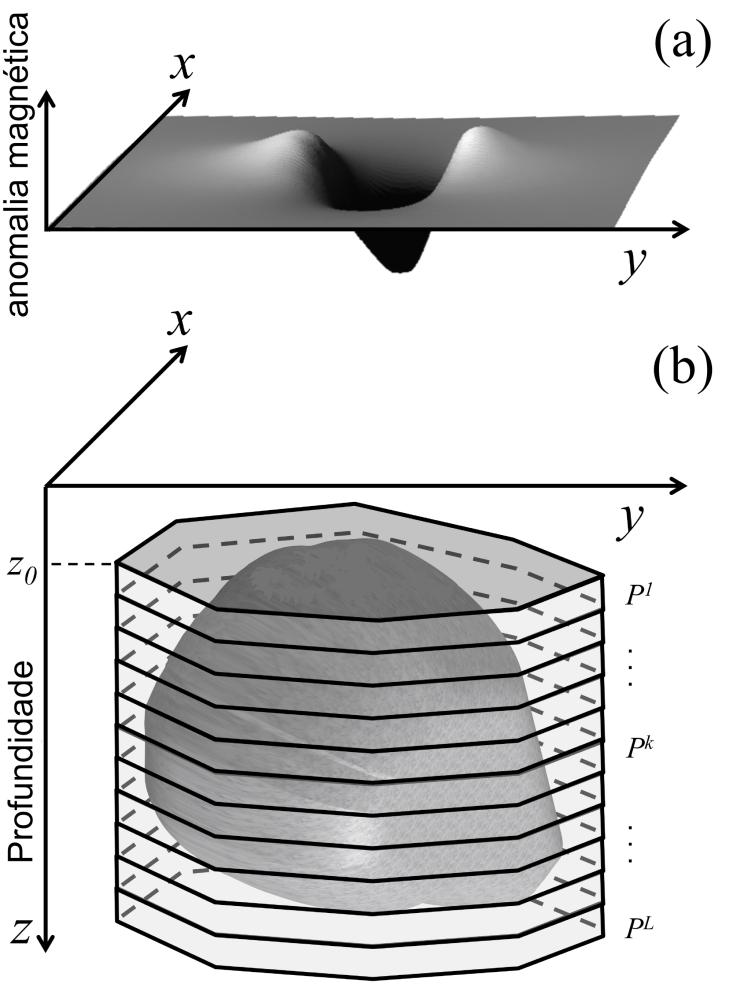
\includegraphics[scale=1]{figures/observed_data.png}
    \caption{Schematic representation (modified from \cite{oliveirajr-barbosa2013}) of (a) total-field anomaly (gray surface) produced by (b) a 3-D anomalous source (dark gray volume). The interpretation model in (b) consists of a set of $L$ vertical, juxtaposed 3-D prisms (light gray) in the vertical direction of a right-handed coordinate system. At the initial iteration, the interpretation model is defined as a vertical cylinder.}
    \label{fig:obs}
\end{figure}

\begin{figure}
    \centering
    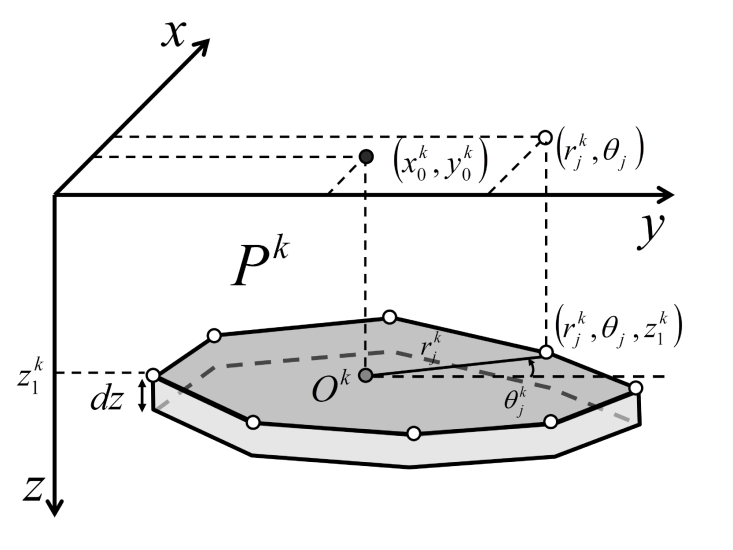
\includegraphics[scale=0.3]{figures/prism_parameters_mod.png}
    \caption{Polygonal cross-section of the $k$th vertical prism described by $V$ vertices (white dots) with radii $r^k_j$, $j = 1, \dots, V$, $k = 1, \dots, L$ , referred to an arbitrary origin $O^k$ (grey dot) with horizontal Cartesian coordinates ($x_0^k$ , $y_0^k$), $k = 1, \dots, L$ , (black dot).}
    \label{fig:prism_parameters}
\end{figure}

% Application to synthetic data - simple model

\begin{figure}
    \centering
    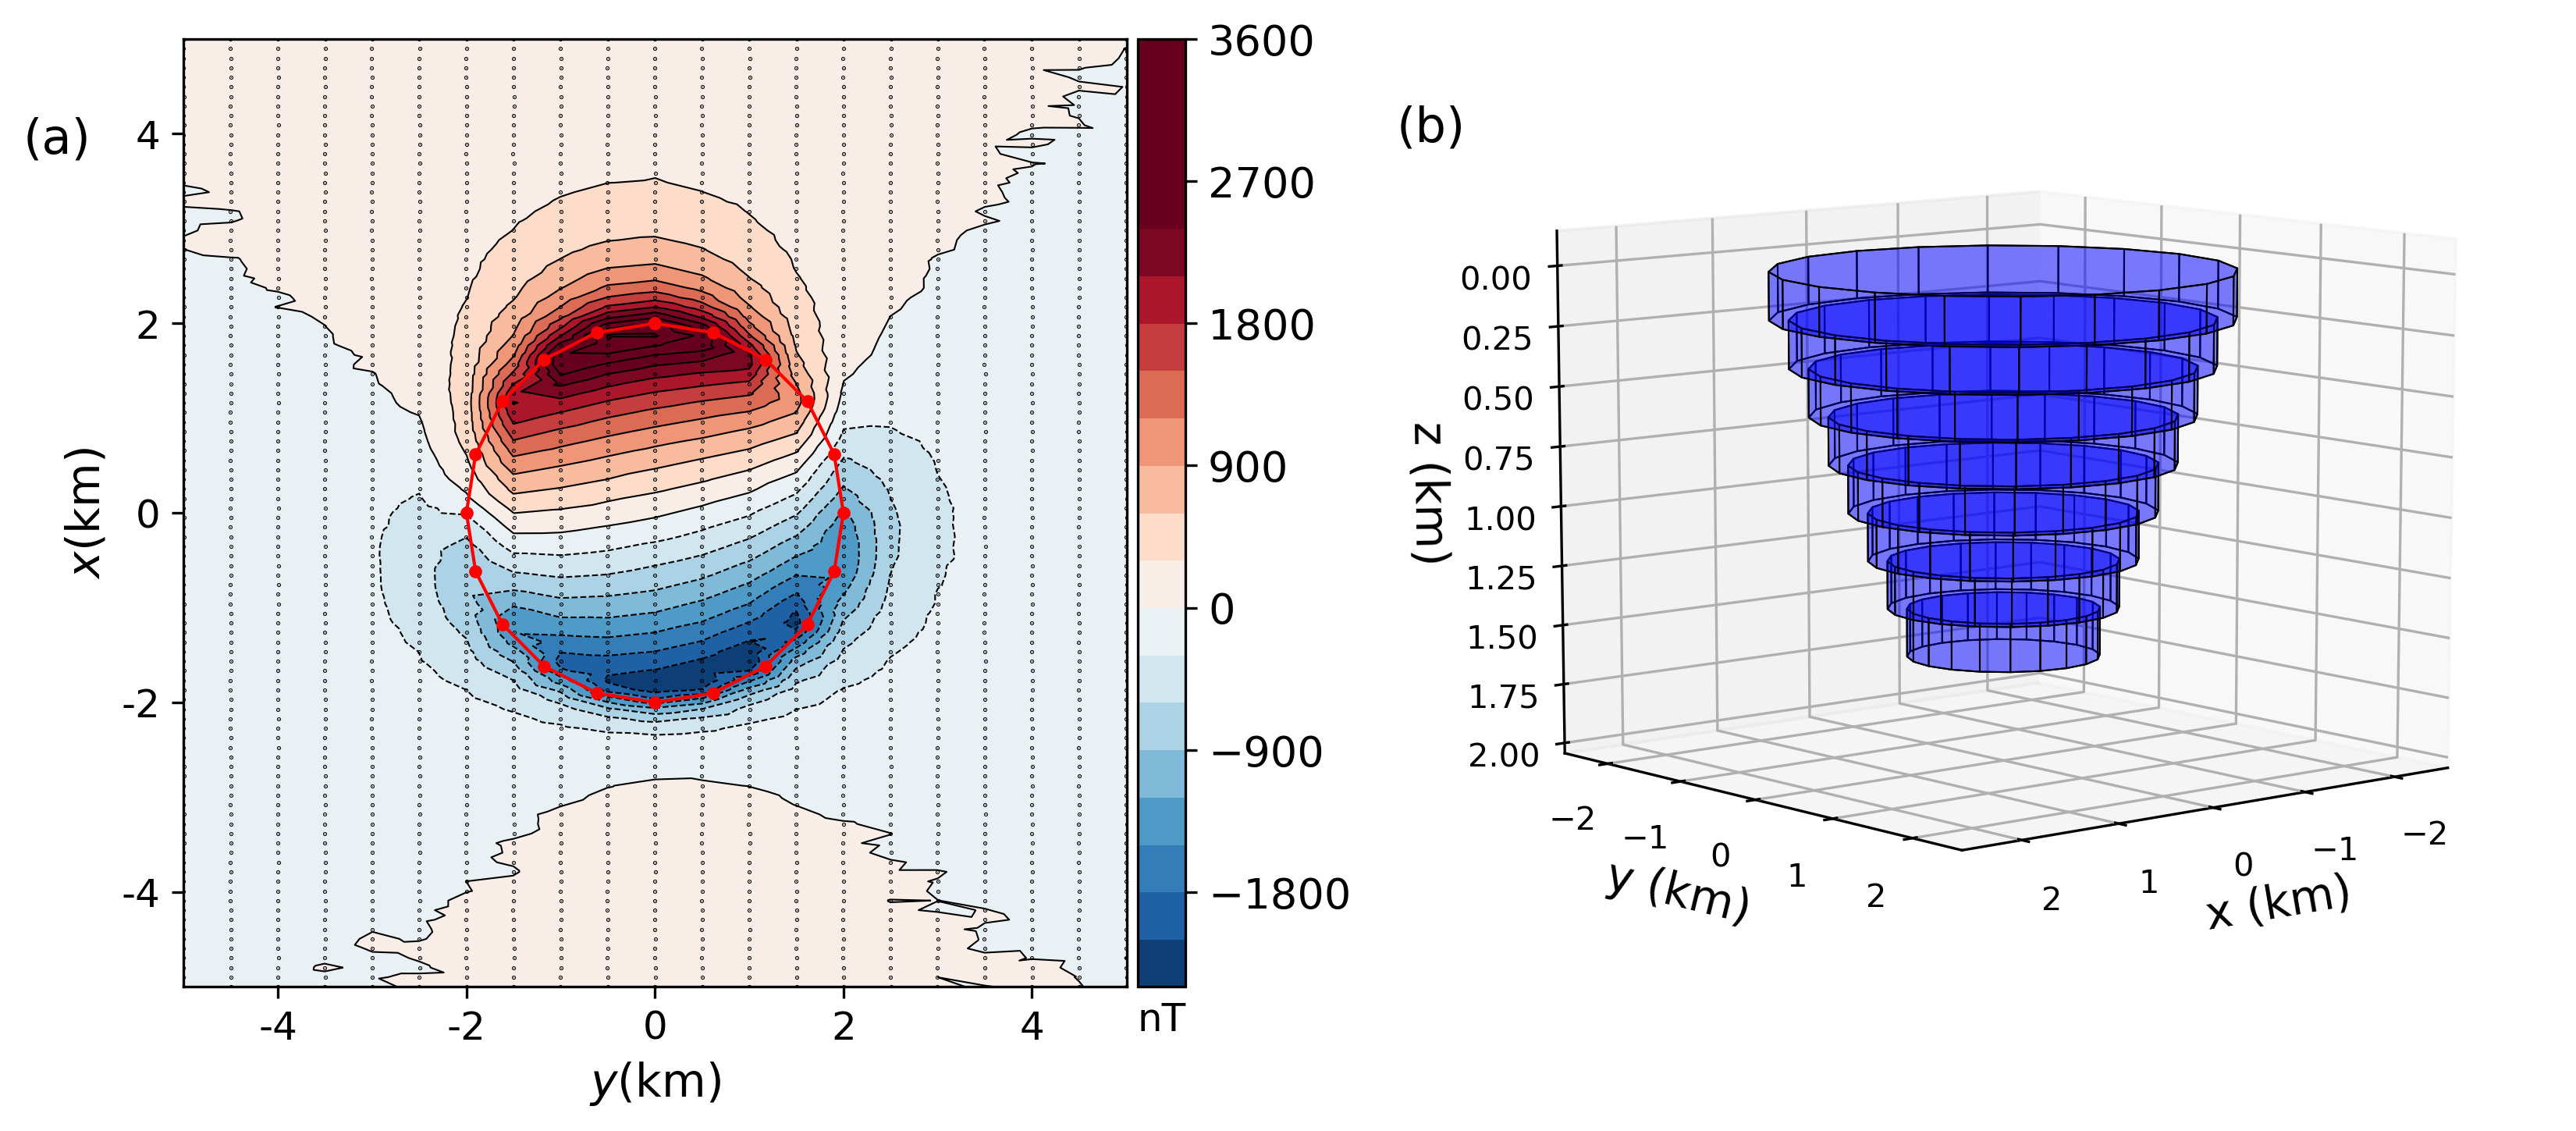
\includegraphics[width=\linewidth]{figures/simple_model_data.png}
    \caption{Simple model simulation. (a) Noise-corrupted total-field anomaly produced by the lopolithic-like body (blue prisms) shown in the panel (b). The black dots represent the observation points. The red circle represents the horizontal projection 
    of the initial approximation $\hat{\mathbf{p}}_{(0)}$
    (red prisms in Fig. \ref{fig:simple_results}b).
    (b) Perspective view of the simple model (lopolithic intrusion) represented by the blue prisms. 
    (c) Discrete map of the goal function $\Gamma(\mathbf{p}, m_0, z_0)$ (Eq.
    \ref{eq:gamma}) produced by the estimates $\hat{\mathbf{p}}_{(f)}$ obtained with
    a $6 \times 6$ grid of tentative values for depth to the top $z_0$ and
    total-magnetization intensity $m_0$.
    The red triangle pinpoint the true and retrieved 	   
    values of $m_0$  and $z_0$. (d) RTP anomaly of the total-field anomaly shown in 
    Fig. \ref{fig:simple_model}a.
}
    \label{fig:simple_model}
\end{figure}

%\begin{figure}
%	\centering
%	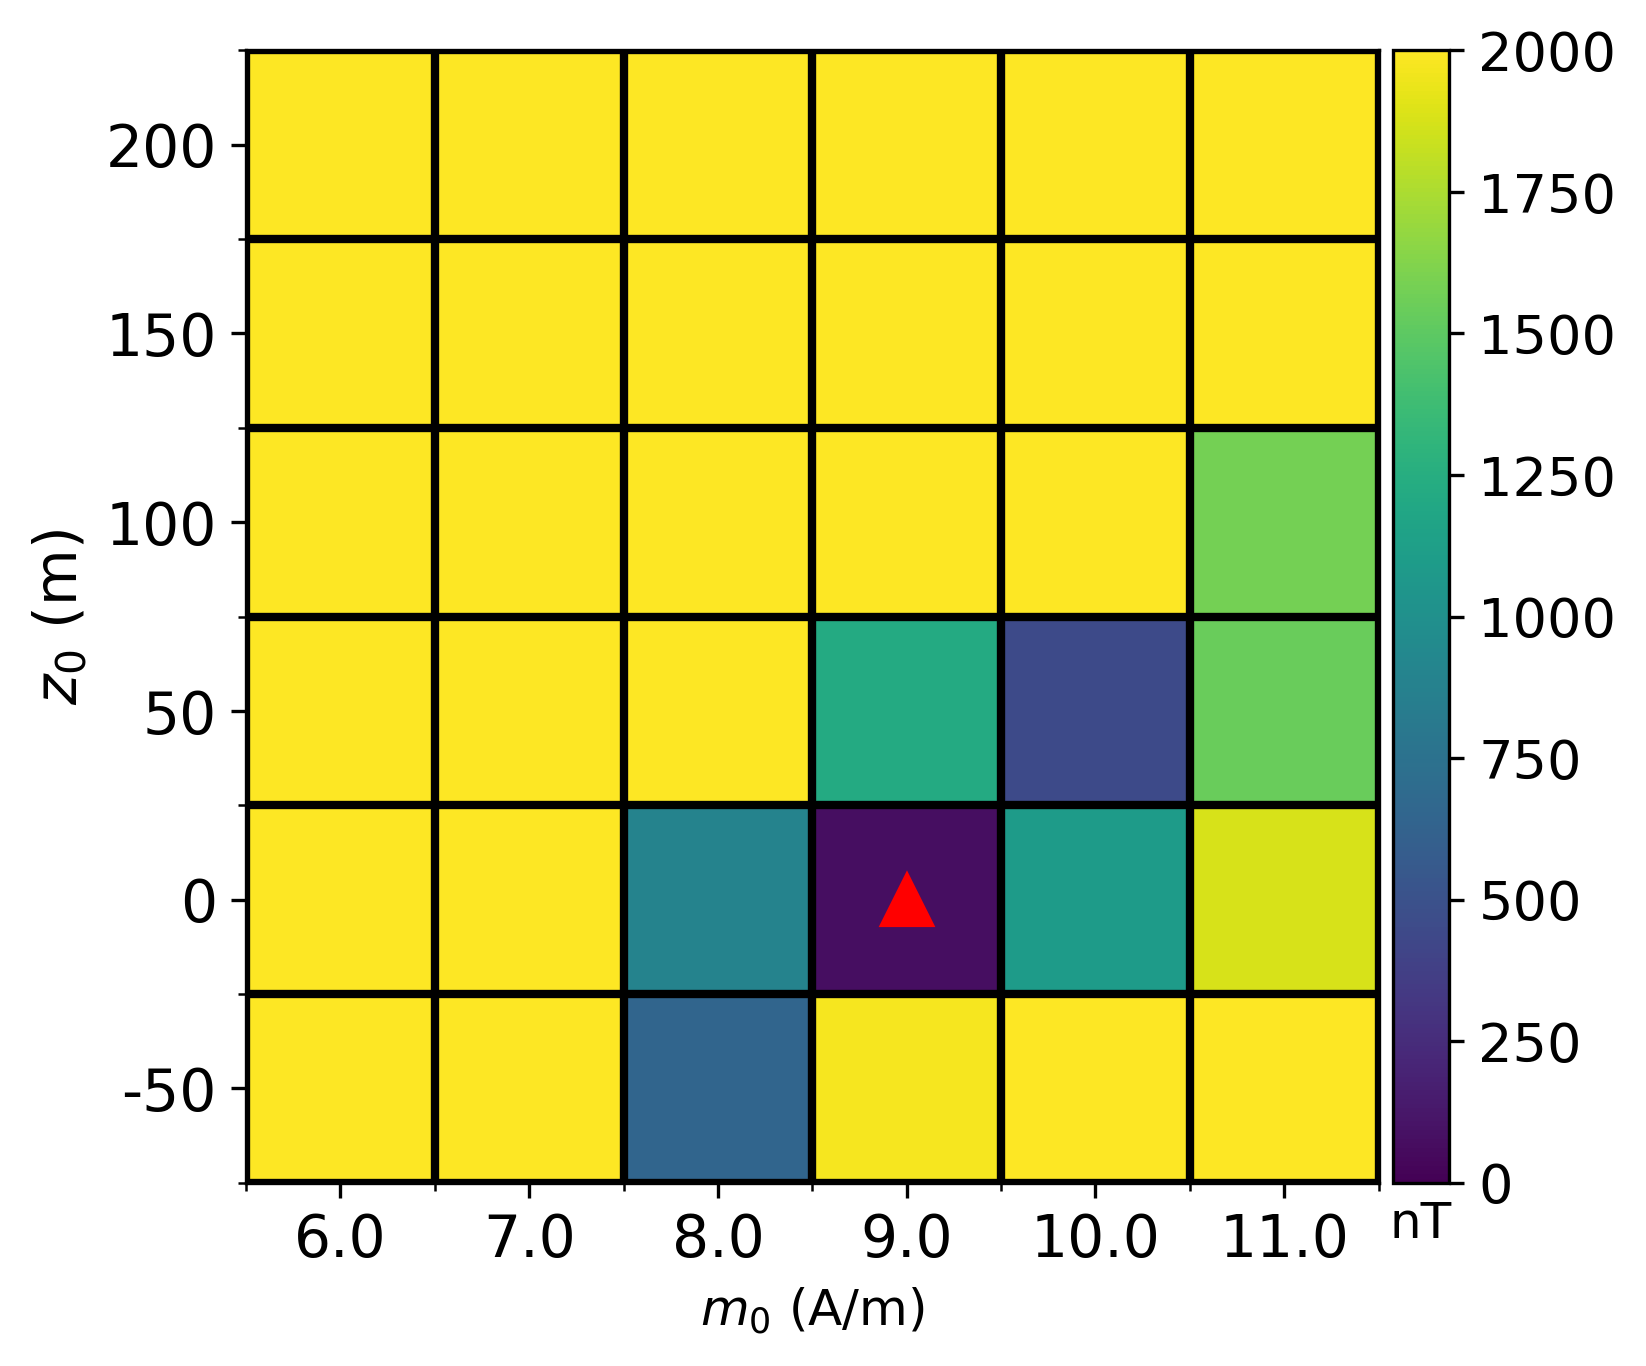
\includegraphics[scale=.75]{figures/simple_gamma.png}
%	\caption{Application to the simple model data. 
%	Discrete map of the goal function $\Gamma(\mathbf{p}, m_0, z_0)$ (Eq. \ref{eq:gamma}) on the plane $ m_0 \times z_0 $,  
%	produced by estimated models with different depths-to-the-top ($ z_0 $) and 
%	total-magnetization intensities ($ m_0 $). 
%	The red triangle represents the $m_0$ and $z_0$ of the true source.}
%	\label{fig:simple_map}
%\end{figure}

\begin{figure}
	\centering
	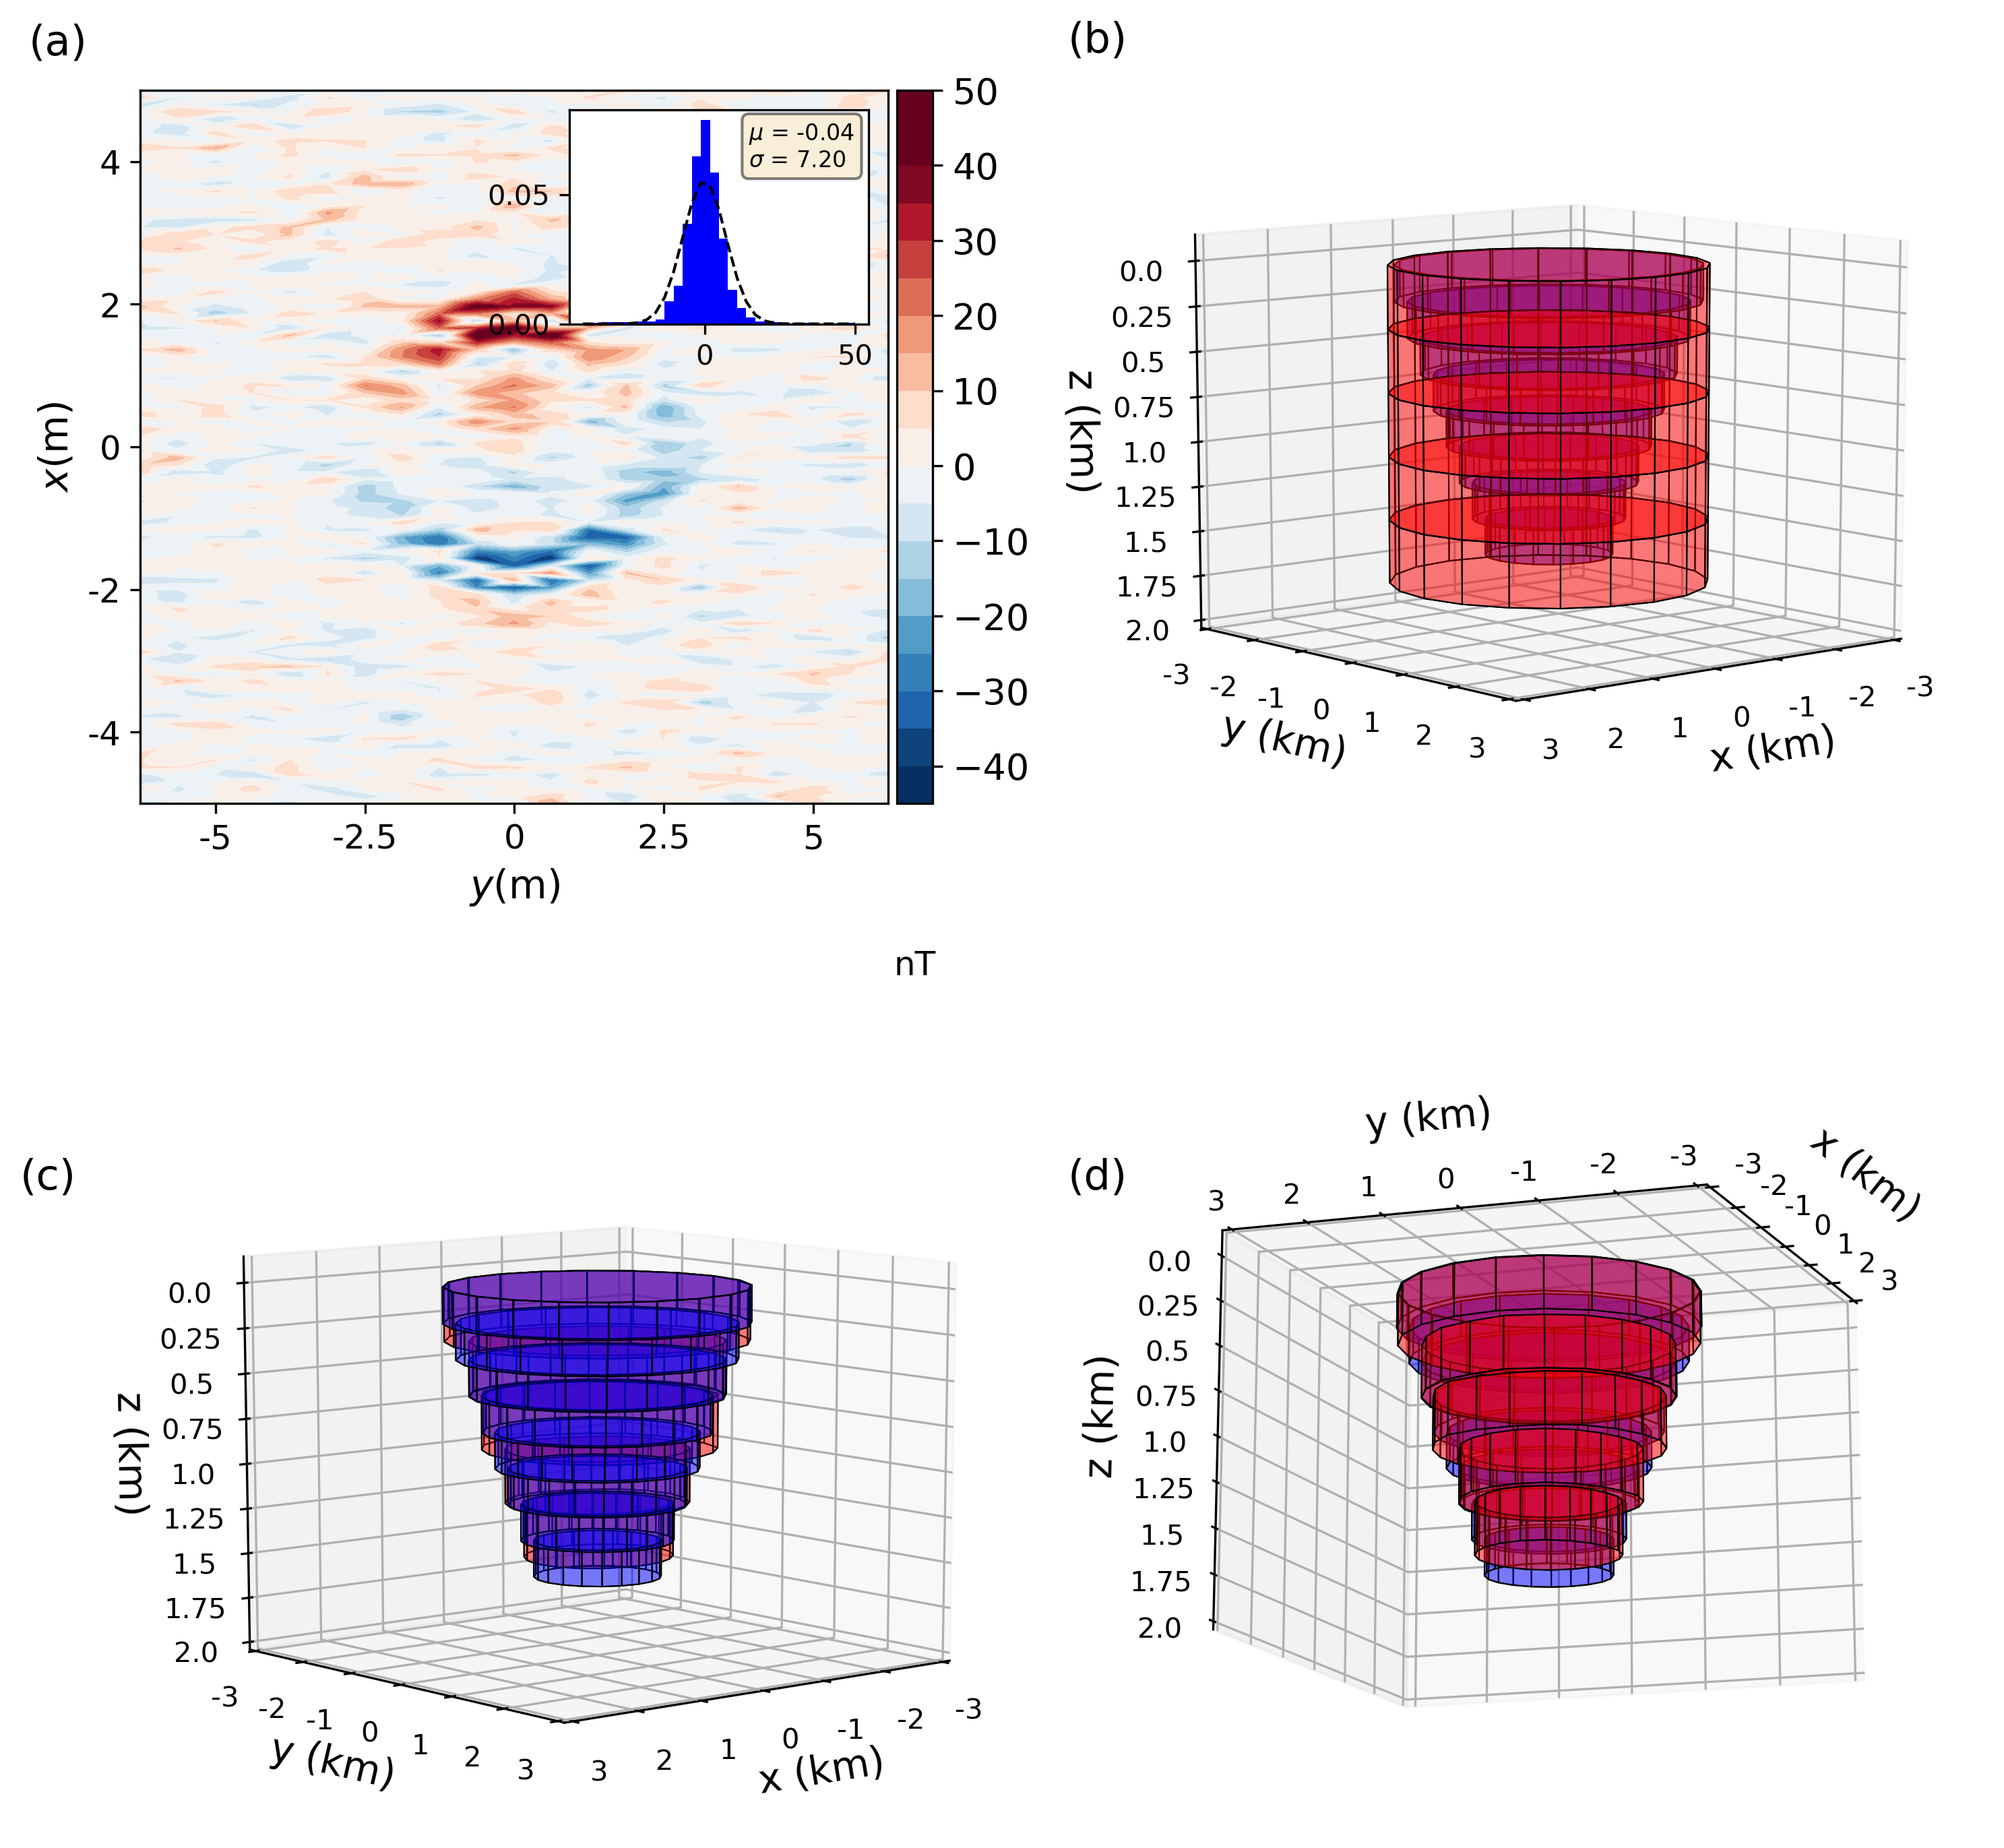
\includegraphics[width=\linewidth]{figures/simple_results.png}
	\caption{Simple model simulation. (a) Residuals between the  noise-corrupted data (Fig. \ref{fig:simple_model}a) and the predicted data (not shown) produced by the estimated model (red prisms shown in the panels (c) and (d)). The inset shows the histogram of the residuals and the Gaussian curve (dashed line) has mean and standard deviation equal to $\mu = -0.04$ nT and $\sigma=7.21$ nT, respectively. (b) Perspective views of the initial approximation (red prisms) and the true model (blue prisms). (c) and (d) Comparison between the estimated source (red prisms) and the true model (blue prisms) in perspective views.}
	\label{fig:simple_results}
\end{figure}

% Application to synthetic data - dipping model

\begin{figure}
    \centering
    \includegraphics[width=\linewidth]{figures/inclined_model_data.png}
    \caption{Dipping model simulation. (a) Noise-corrupted total-field anomaly produced by the dipping model (blue prisms shown in the panels (c) and (d)). The black dots represent the observation points. The red circle represents the horizontal projection 
   	of the initial approximation $\hat{\mathbf{p}}_{(0)}$ 
   	(red prisms in Fig. \ref{fig:dipping_results}). The blue polygon is the horizontal projection of the simulated dipping source.
   	(b) Vertical coordinates of the observations simulating an airborne survey. (c) and (d) Perspective views of the dipping model represented by the blue prisms.
}
    \label{fig:dipping_model}
\end{figure}

\begin{figure}
    \centering
    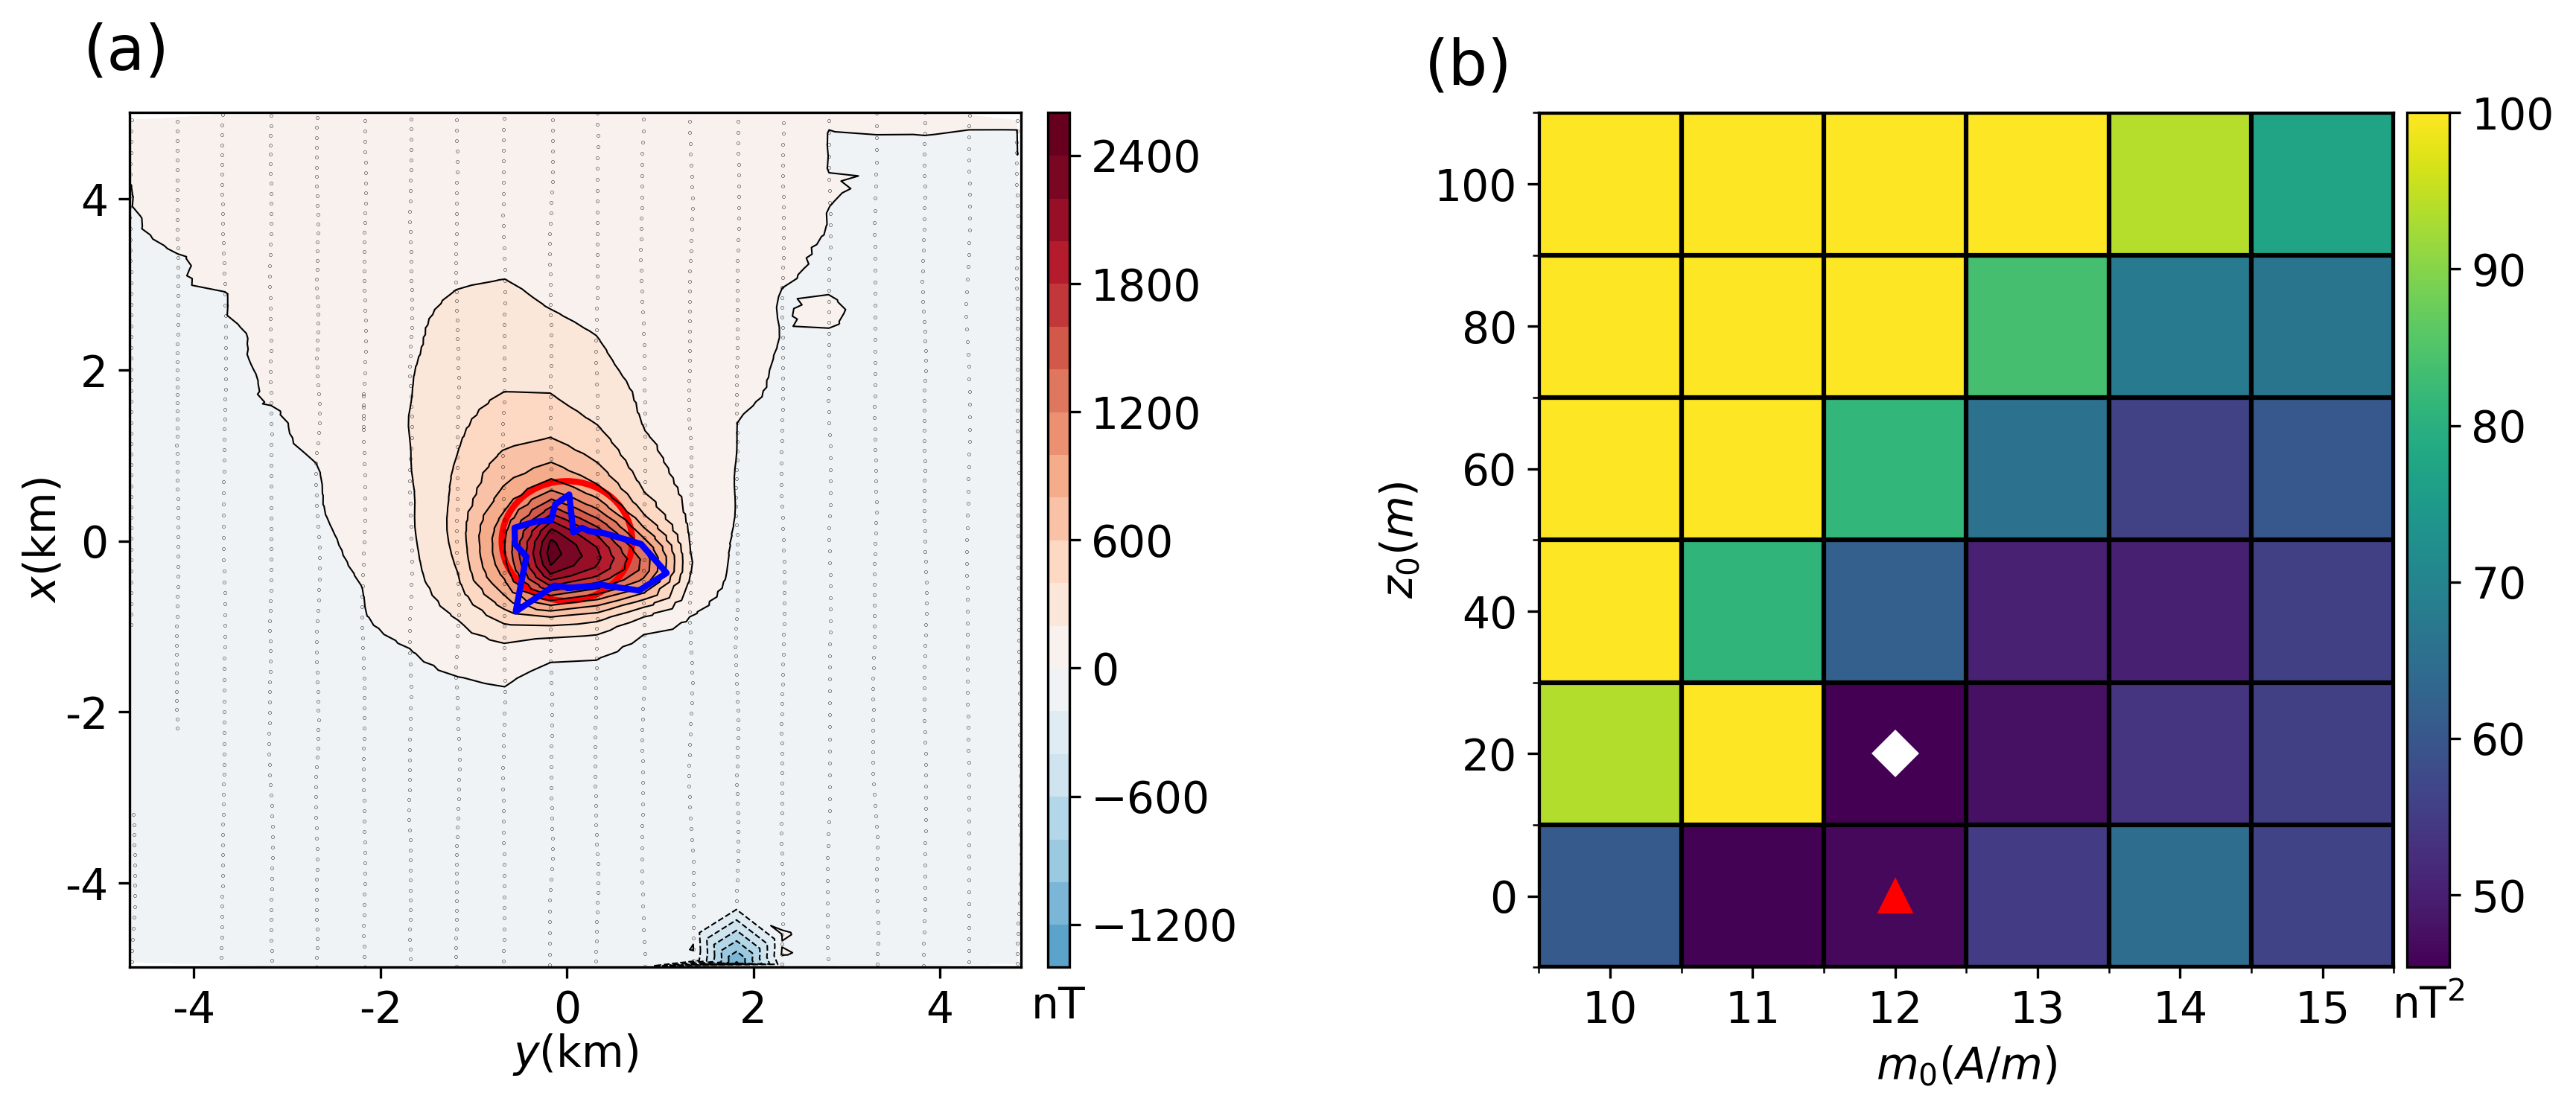
\includegraphics[width=\linewidth]{figures/inclined_rtp.png}
    \caption{Dipping model simulation. (a) RTP anomaly of the total-field anomaly
    shown in Fig. \ref{fig:dipping_model}(a). 
	The red circle and the blue polygon represent the horizontal projections of
	the initial approximation $\hat{\mathbf{p}}_{(0)}$ and  the simulated dipping
	source, respectively.
	(b) Discrete map of the goal function $\Gamma(\mathbf{p}, m_0, z_0)$ (Eq.
	\ref{eq:gamma}) produced by the estimates $\hat{\mathbf{p}}_{(f)}$ obtained with
	a $6 \times 6$ grid of tentative values for depth to the top $z_0$ and
	total-magnetization intensity $m_0$.
	The red triangle  and white diamond pinpoint, respectively, the true and
	retrieved values of $m_0$  and $z_0$.     
}
    \label{fig:dipping_rtp}
\end{figure}


\begin{figure}
    \centering
    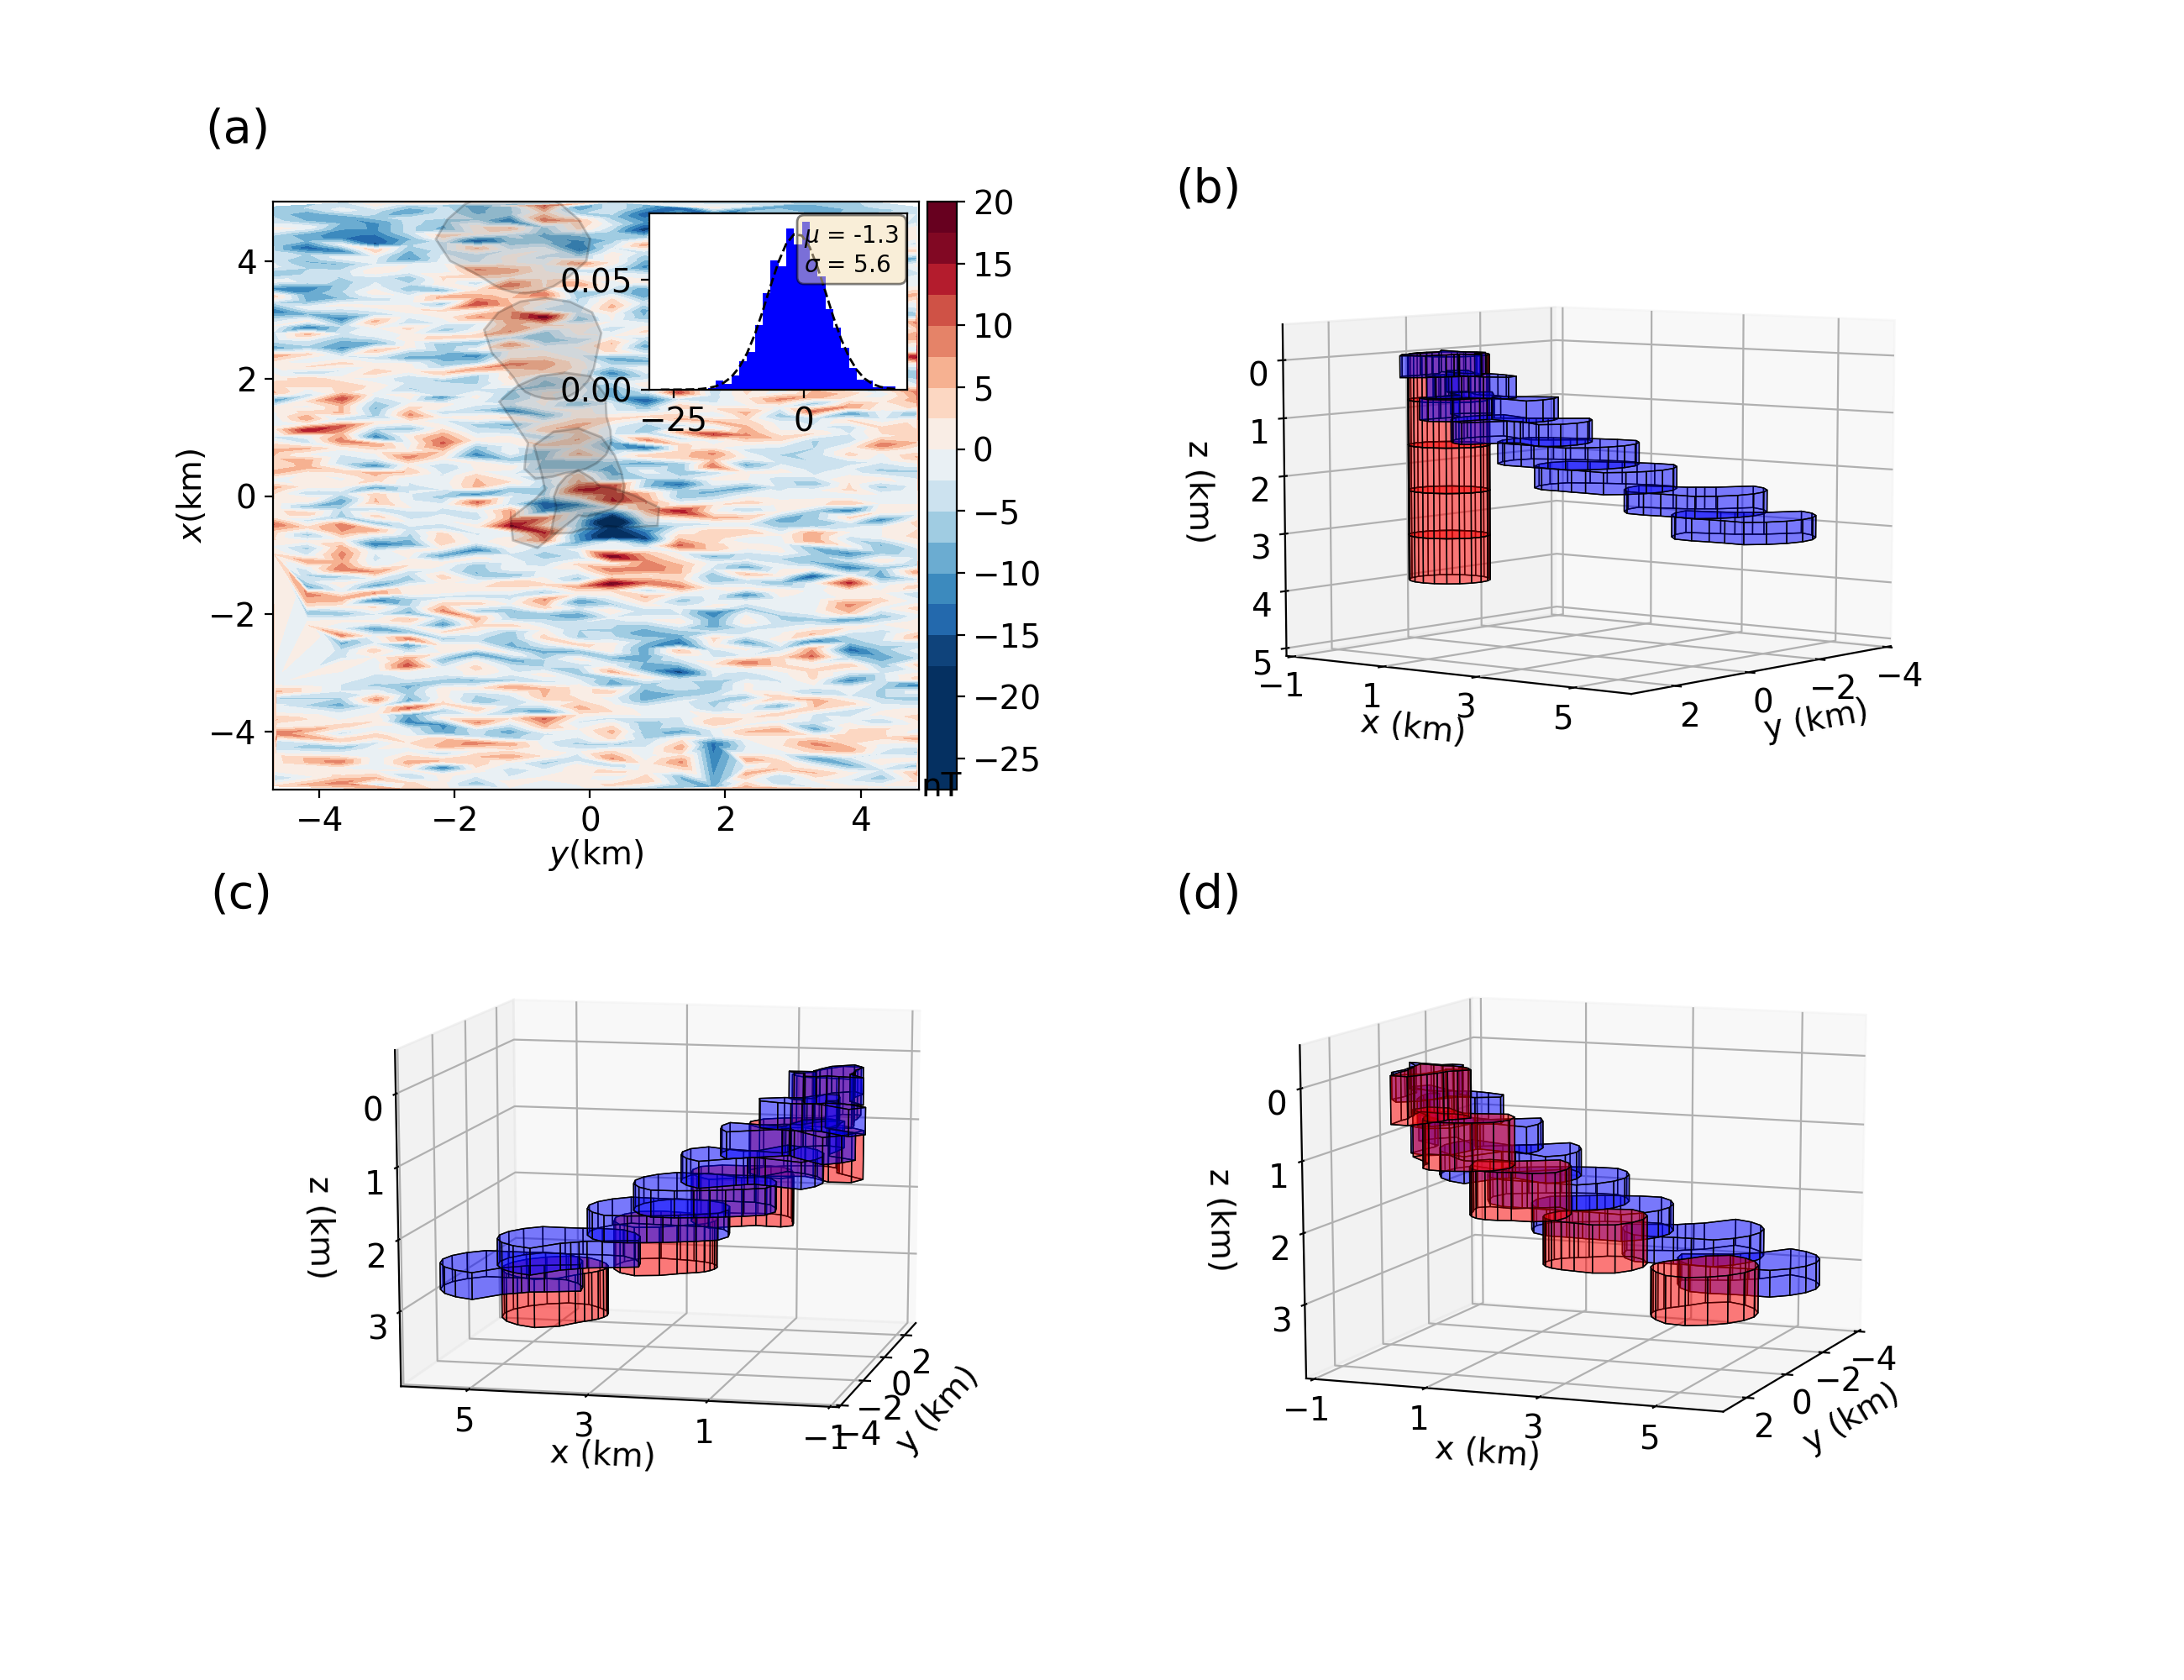
\includegraphics[width=\linewidth]{figures/inclined-l2-solution.png}
    \caption{Dipping model simulation. (a) Residuals between the  noise-corrupted data (Fig. \ref{fig:dipping_model}a) and the predicted data (not shown) produced by the estimated model (red prisms shown in the panels (c) and (d)) using $m_0$  and $z_0$ pinpointed by the white diamond in Fig. \ref{fig:dipping_rtp}b. The inset shows the histogram of the residuals and the Gaussian curve (dashed line) has mean and standard deviation equal 
    to $\mu = 1.3$ nT and $\sigma=5.6$ nT, respectively. 
    The gray polygons are the horizontal projections of the estimated source (red prisms in panels (c) and (d)).
     (b) Perspective views of the initial approximation (red prisms) and the true model (blue prisms). 
     (c) and (d) Comparison between the estimated source (red prisms) and the true model (blue prisms) in perspective views.     
}
    \label{fig:dipping_results}
\end{figure}


% Application to synthetic data - Dipping model in the presence of a regional field test

\begin{figure}
    \centering
    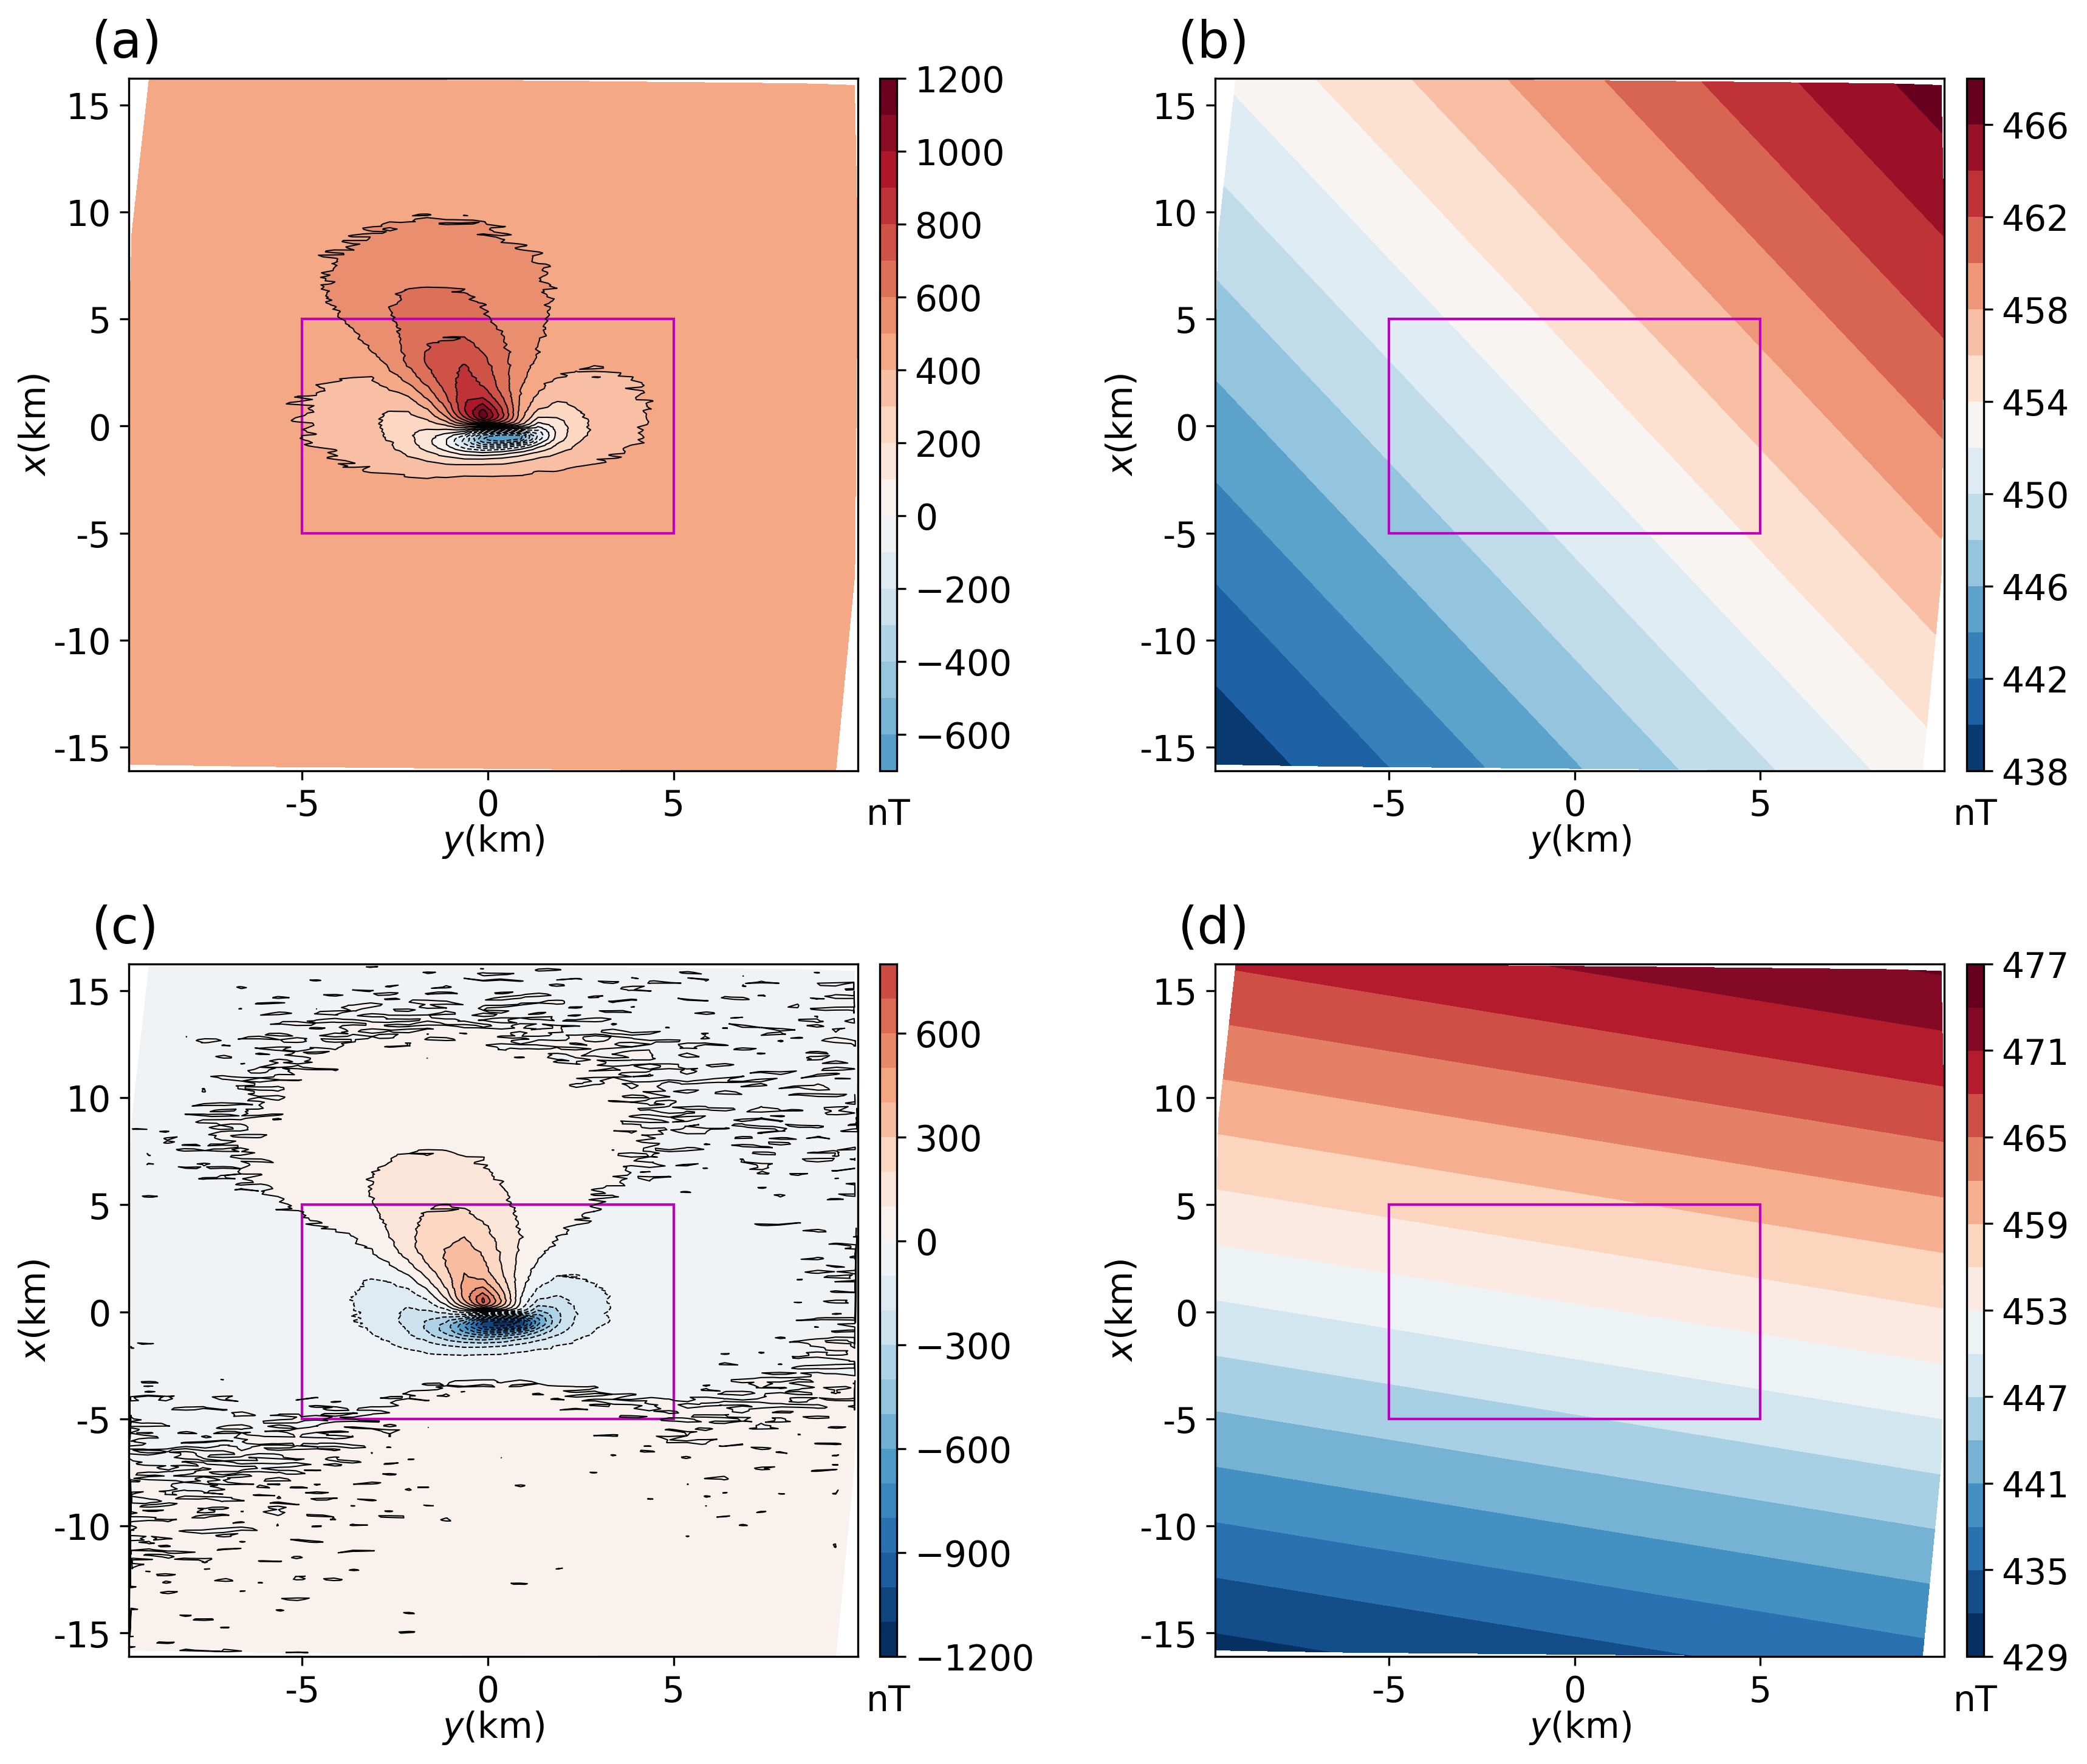
\includegraphics[width=\linewidth]{figures/regional-data-large.png}
    \caption{Dipping model with regional field simulation. (a) Noise-corrupted total-field anomaly composed of a simulated residual field (Fig. \ref{fig:dipping_model}a) due to 
dipping model (blue prisms shown in Fig. \ref{fig:dipping_model}c and d) and a regional field (shown in panel (b)). (b) Simulated regional field through a first-order polynomial. 
(c) Residual total-field anomaly after subtracting from the original anomaly (shown in panel (a)) a
regional total-field anomaly (shown in panel (d)) obtained by a least-squares polynomial fitting. 
(d)  Regional total-field anomaly approximated by a least-squares polynomial fitting to the original anomaly (shown in panel (a)). The magenta rectangle delimits the data to be inverted.
}
    \label{fig:dipping_regional_model}
\end{figure}

\begin{figure}
    \centering
    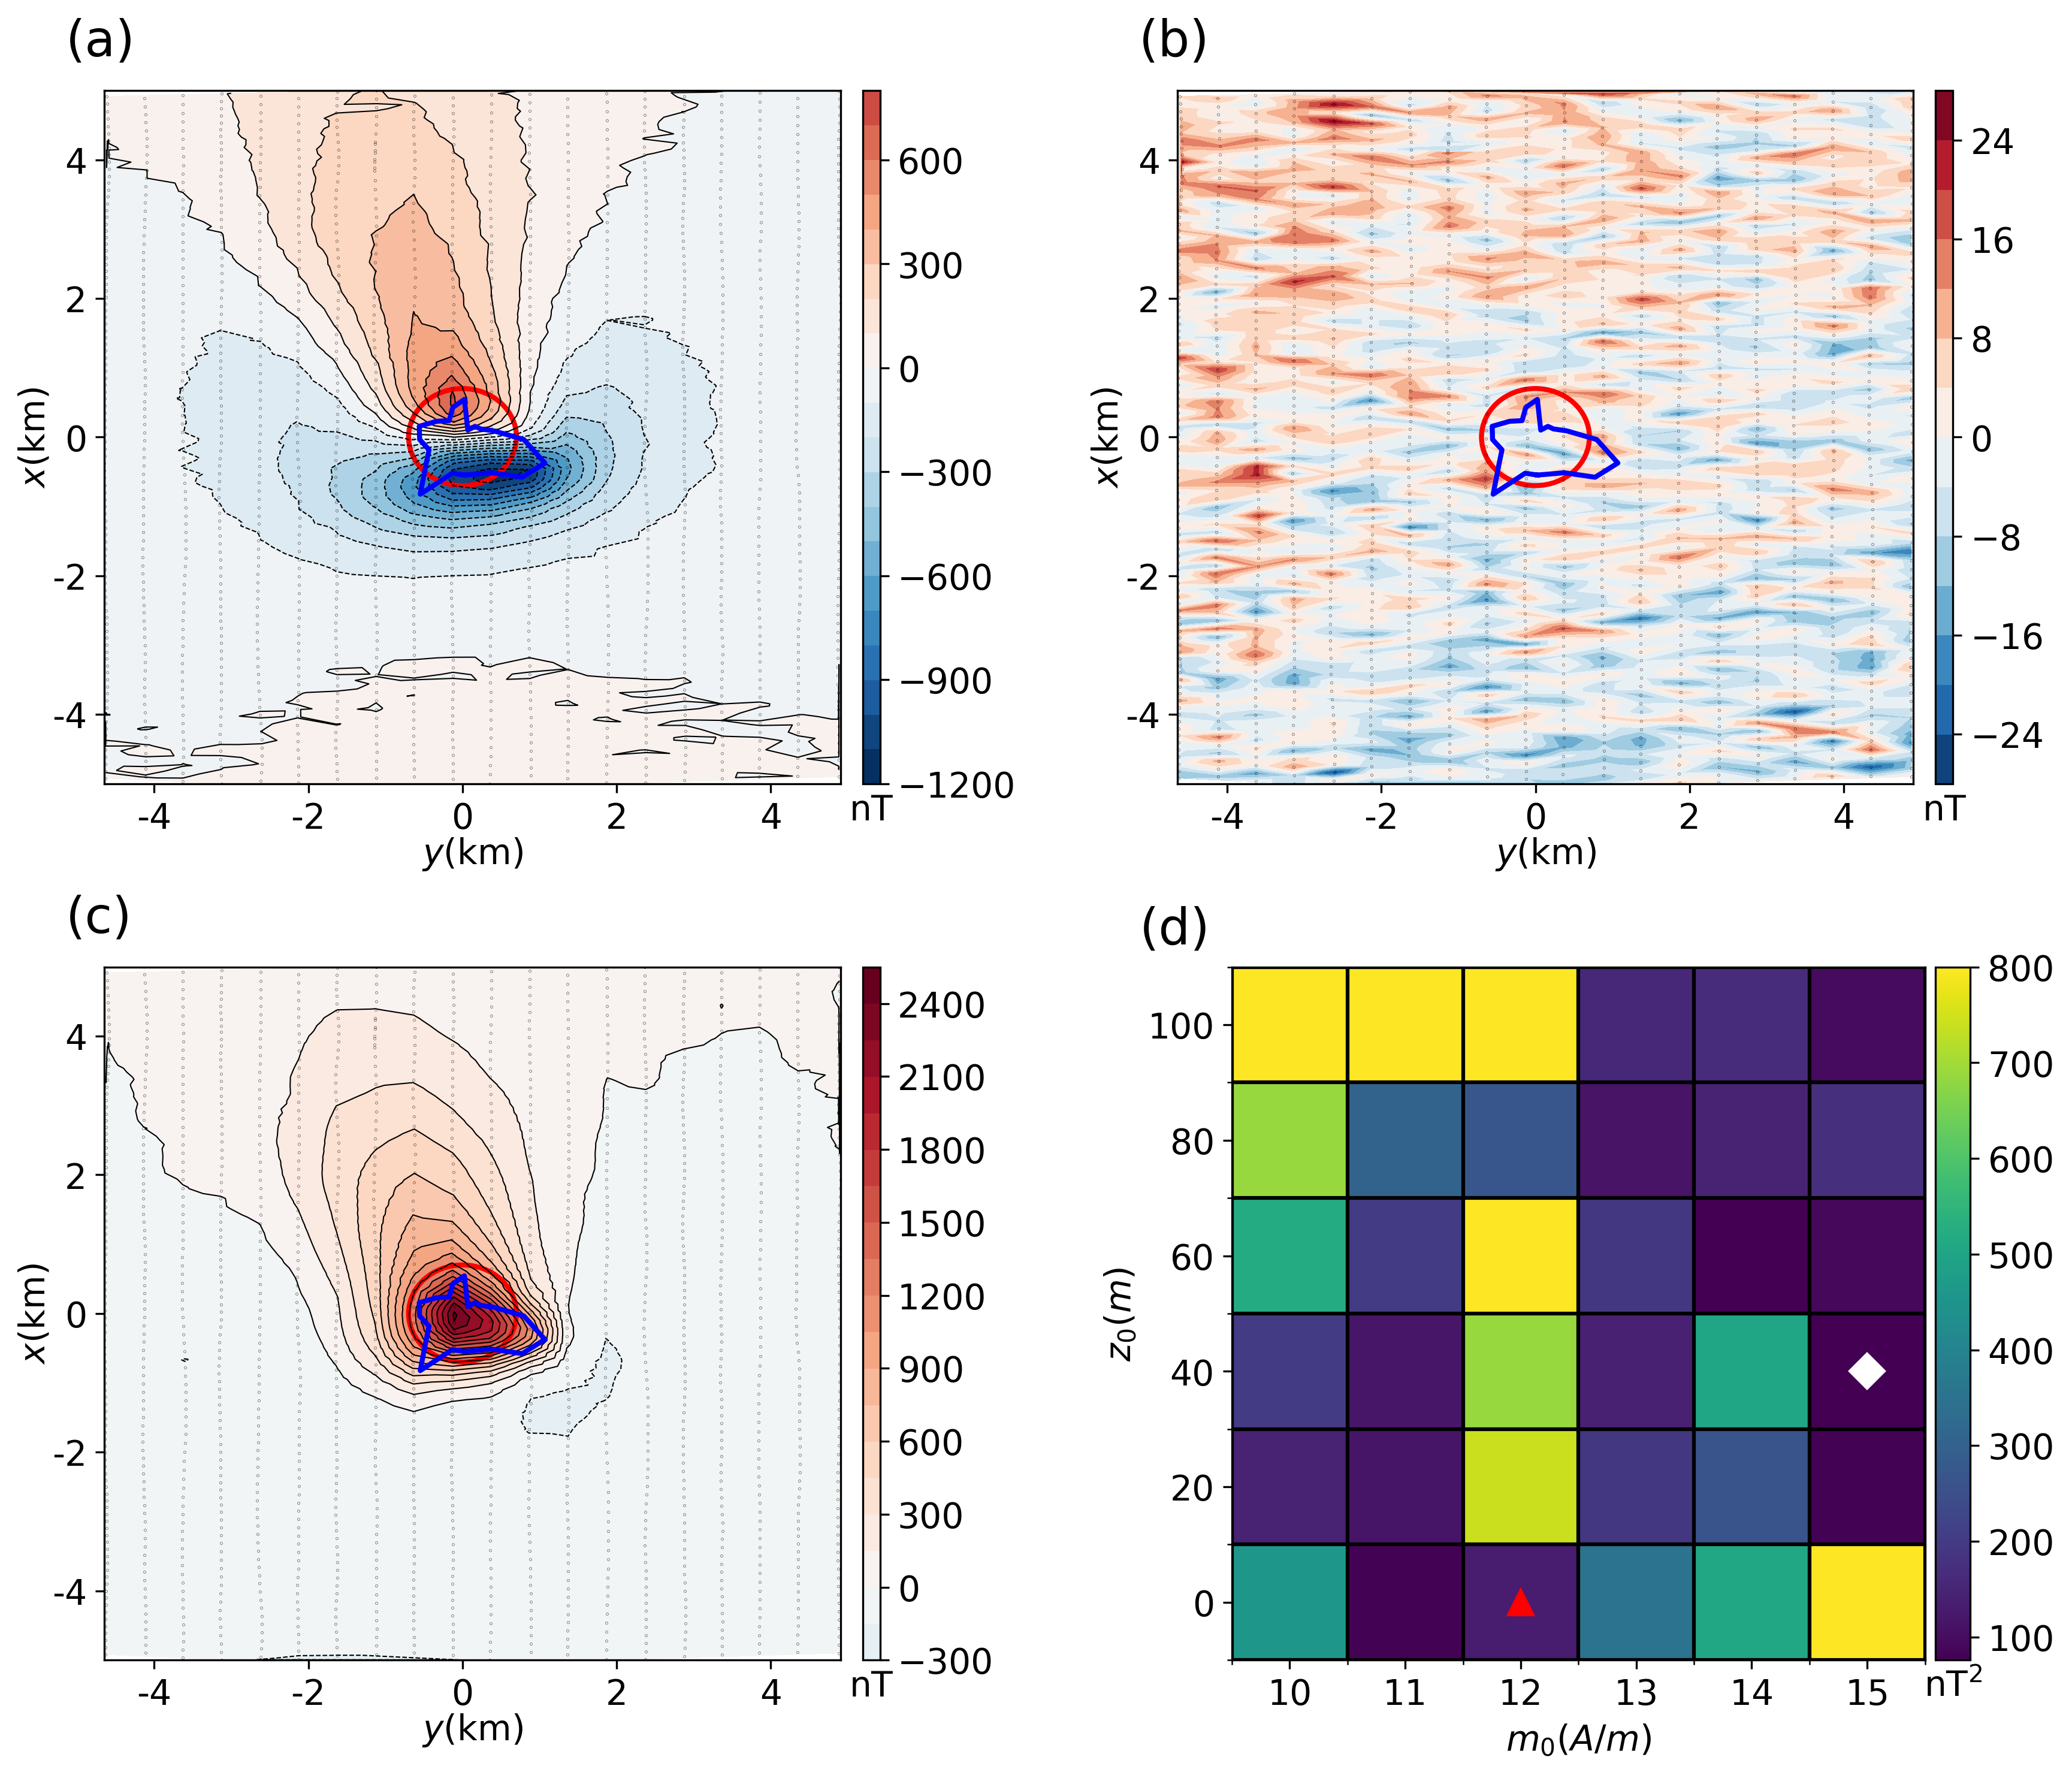
\includegraphics[width=\linewidth]{figures/regional_rtp.png}
    \caption{Dipping model with regional field simulation. (a) Residual total-field
    anomaly to be inverted over the area delimited by the  magenta rectangle 
    in Fig. \ref{fig:dipping_regional_model}(c). 
    (b) Differences between the total-field anomaly produced by the dipping model
    (Fig. \ref{fig:dipping_model}a) and the residual total-field anomaly (shown in
    panel (a)) after a regional-residual separation using a least-squares polynomial
    fitting. 
    (c) RTP anomaly of the  residual total-field anomaly shown in panel (a). 
    (d) Discrete map of the goal function $\Gamma(\mathbf{p}, m_0, z_0)$ (Eq.
    \ref{eq:gamma}) produced by the estimates $\hat{\mathbf{p}}_{(f)}$ obtained with
    a $6 \times 6$ grid of tentative values for depth to the top $z_0$ and
    total-magnetization intensity $m_0$.
    The red triangle  and white diamond pinpoint, respectively, the true and
    retrieved values of $m_0$  and $z_0$.
    In the panels (a)-(c), the red circle and the blue polygon represent the
    horizontal projections of the initial approximation $\hat{\mathbf{p}}_{(0)}$ 
    and the simulated dipping source, respectively.
}
    \label{fig:dipping_regional_rtp}
\end{figure}


\begin{figure}
    \centering
    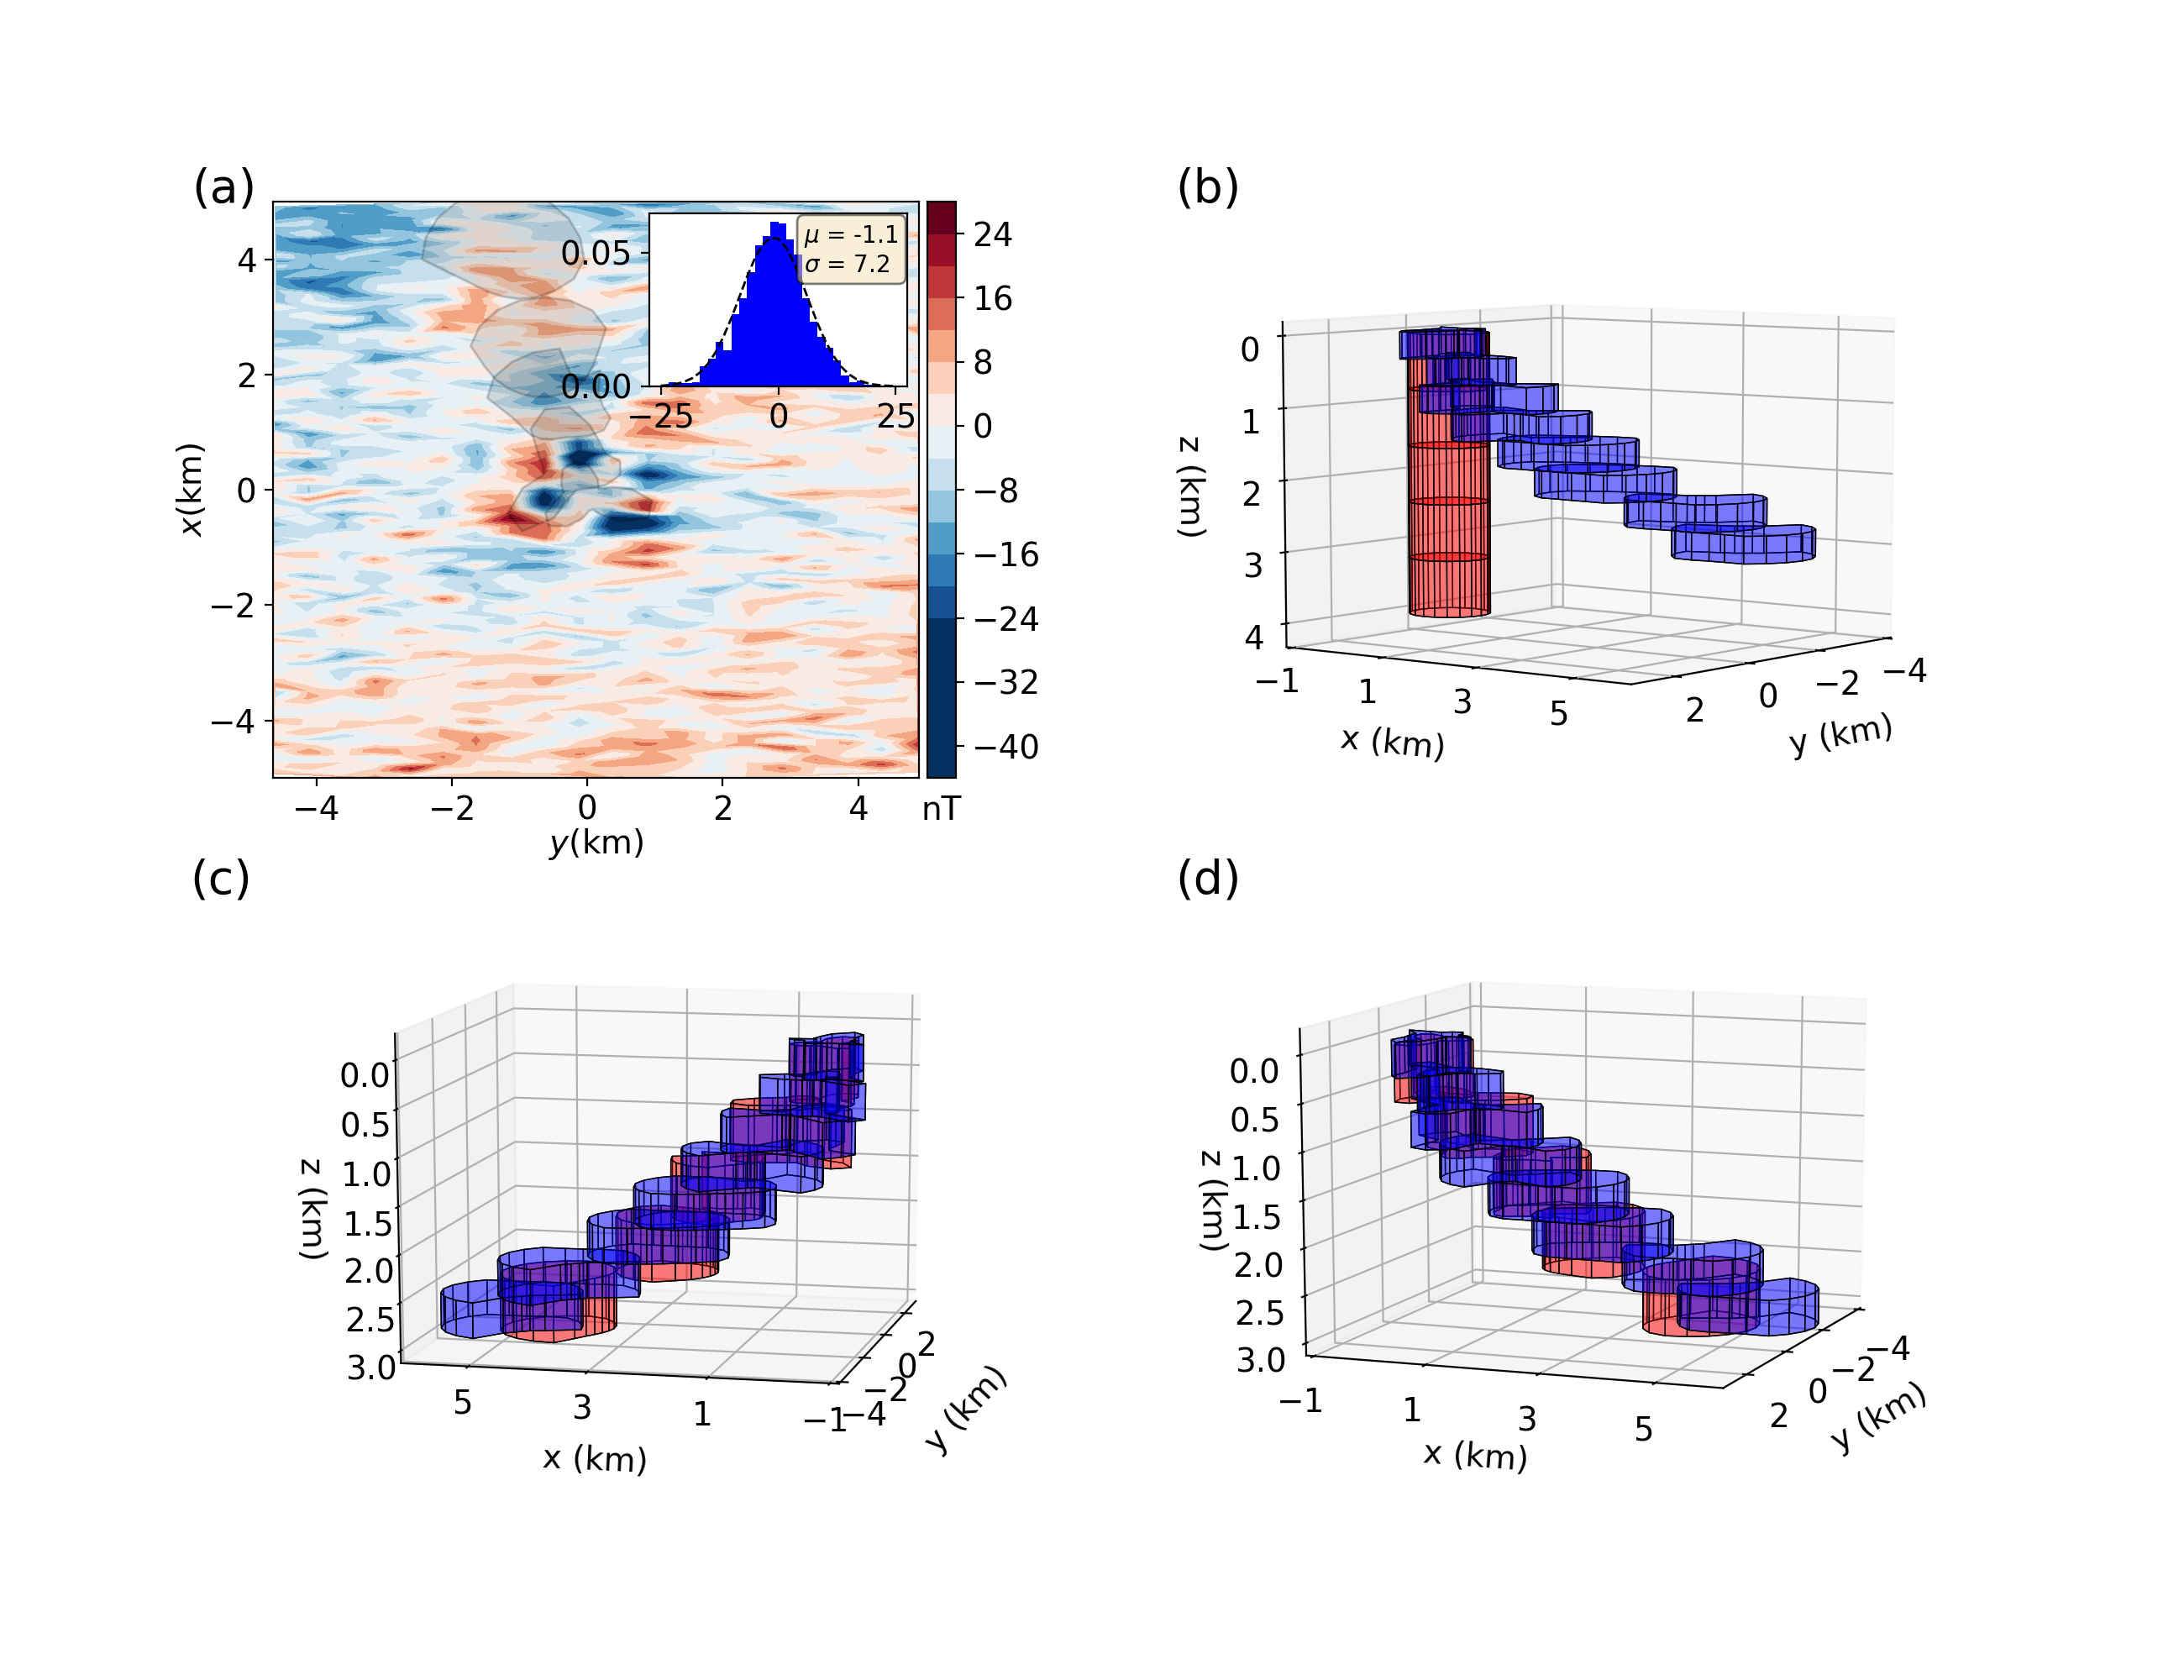
\includegraphics[width=\linewidth]{figures/regional-l2-solution.png}
    \caption{Dipping model with regional field simulation. (a) Residuals between the  noise-corrupted data (Fig. \ref{fig:dipping_regional_rtp}a) and the predicted data (not shown) produced by the estimated model (red prisms shown in the panels (c) and (d)) using 
$m_0$  and $z_0$ pinpointed by the white diamond in Fig. \ref{fig:dipping_regional_rtp}d.
The inset shows the histogram of the residuals and the Gaussian curve (dashed line) has mean and standard deviation equal   to $\mu = -4.4$ nT and $\sigma=7.8$ nT, respectively. 
    The gray polygons are the horizontal projections of the estimated source (red prisms in panels (c) and (d)).
     (b) Perspective views of the initial approximation (red prisms) and the true model (blue prisms). 
     (c) and (d) Comparison between the estimated source (red prisms) and the true model (blue prisms) in perspective views.     
}
    \label{fig:regional-results}
\end{figure}

% Application to synthetic data - complex model

\begin{figure}
    \centering
    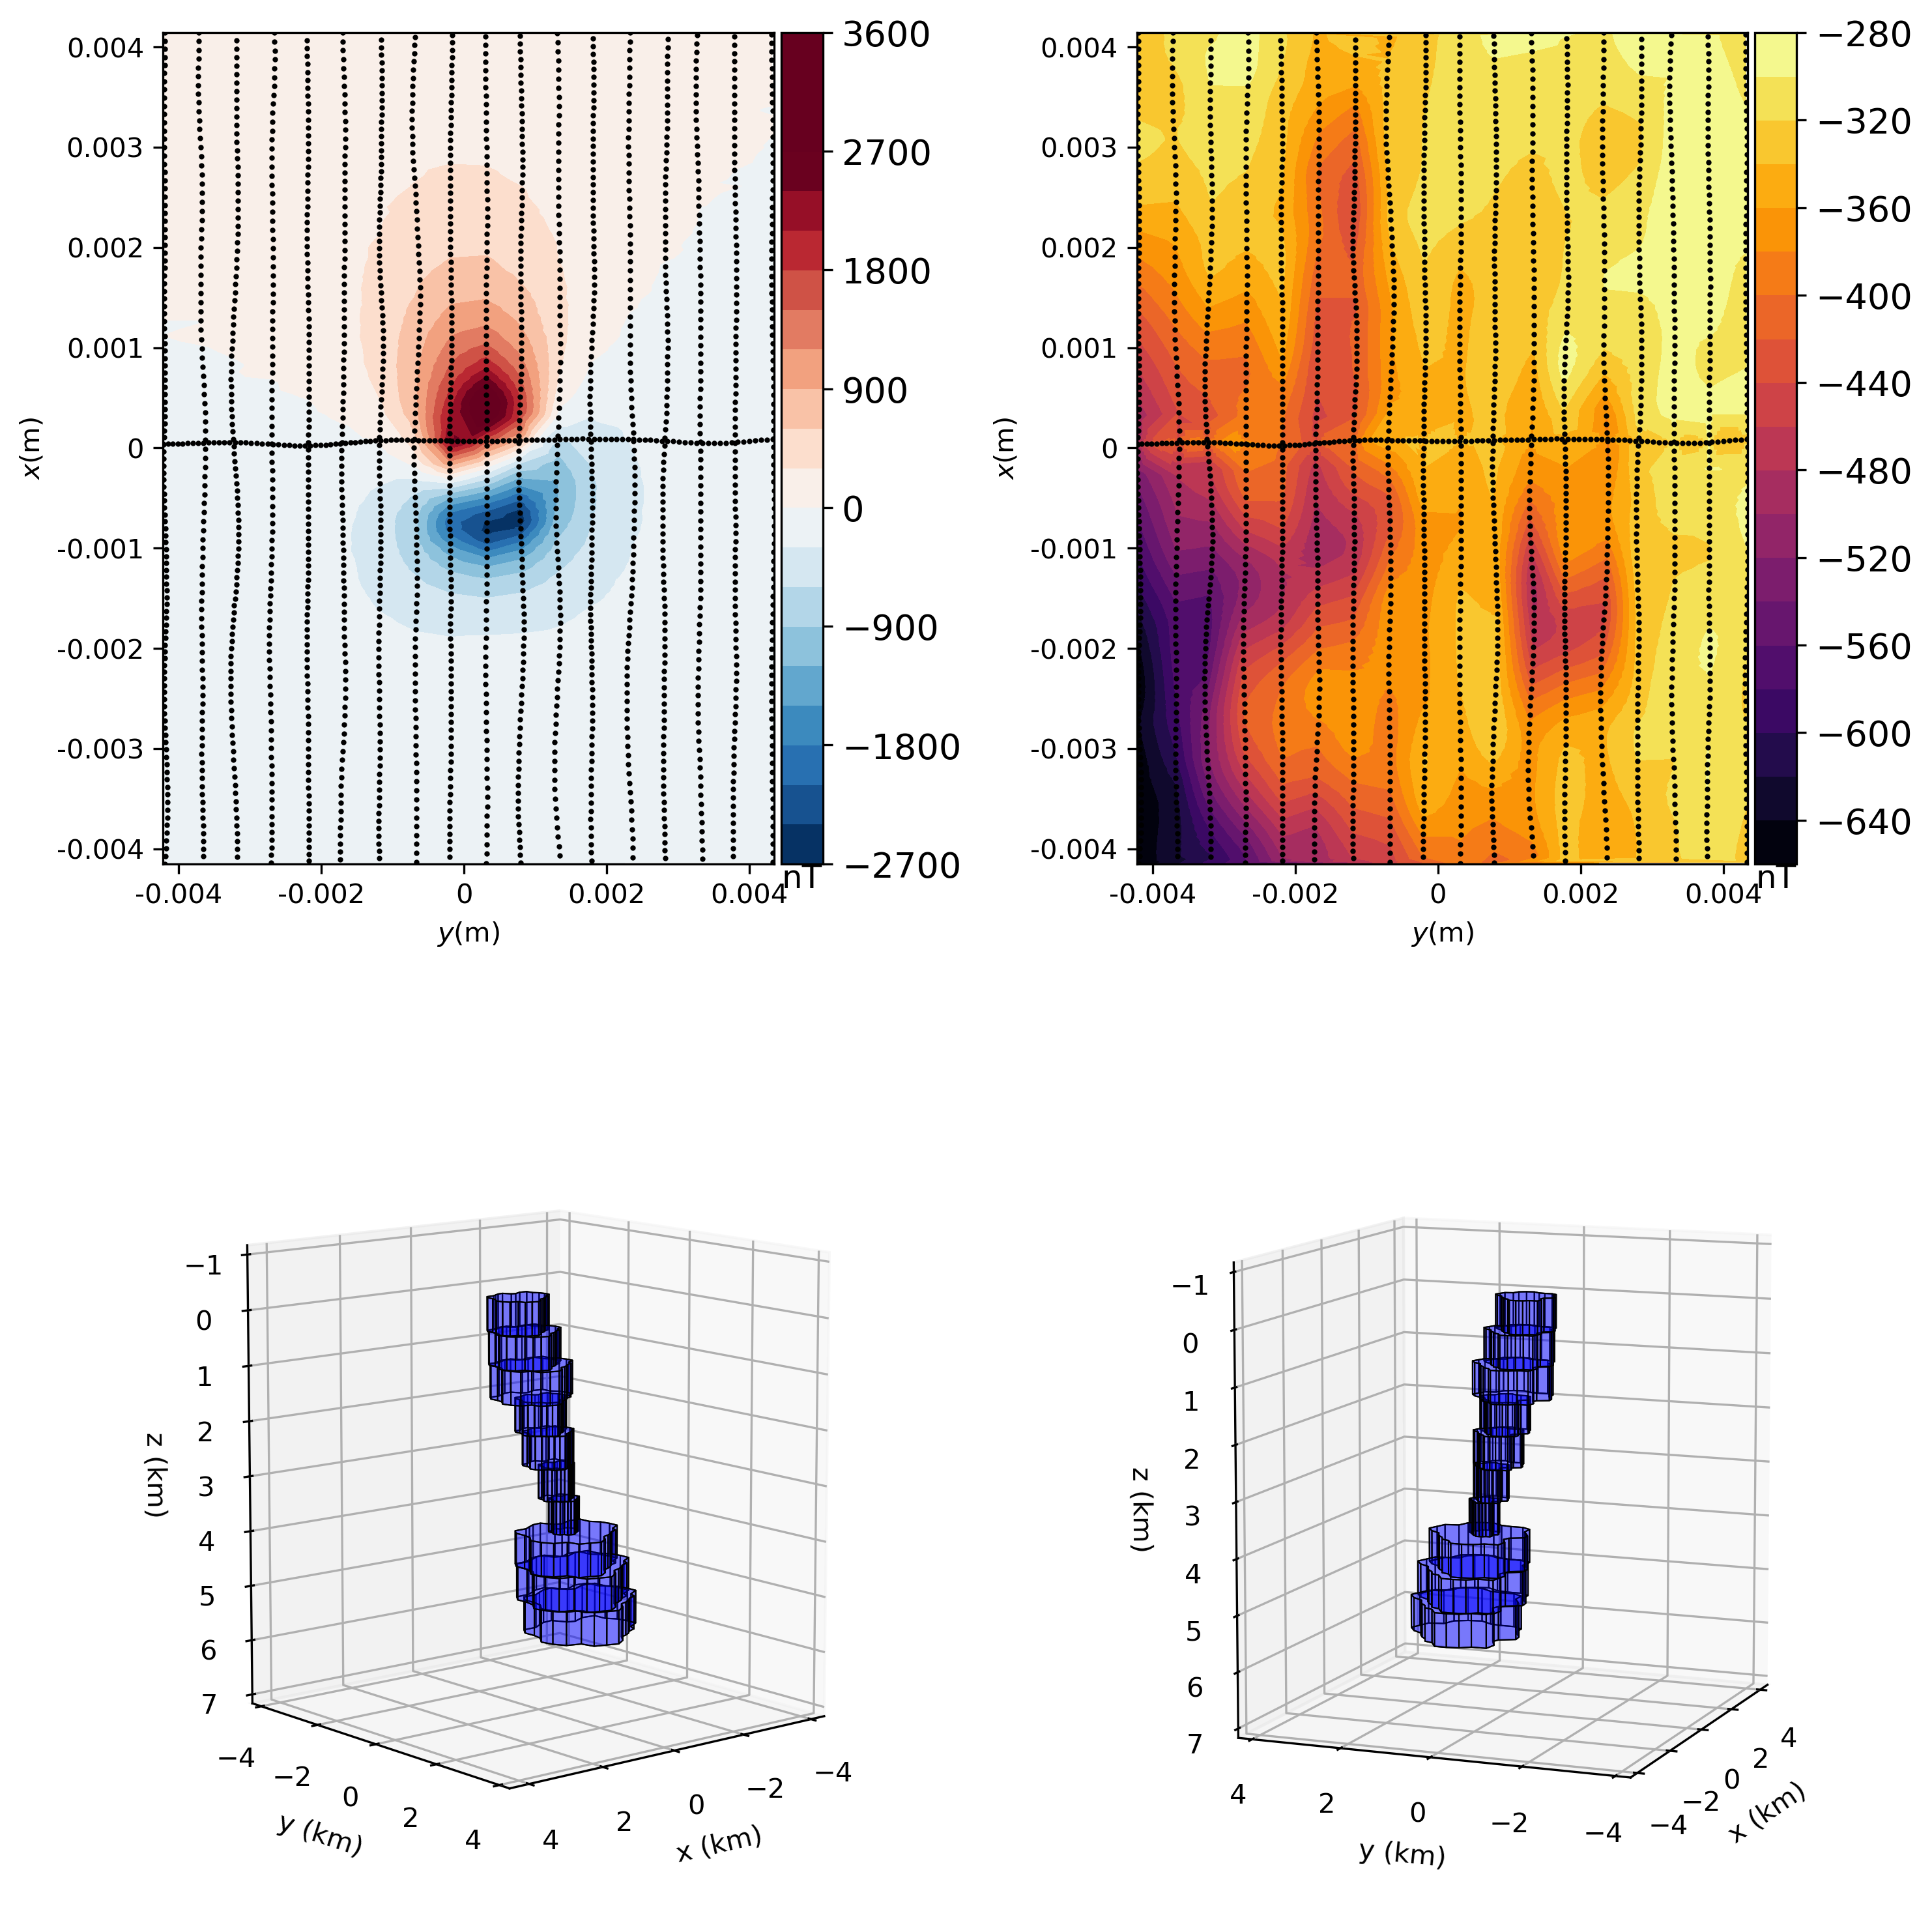
\includegraphics[width=\linewidth]{figures/complex_model_data.png}
    \caption{Complex model simulation. (a) Noise-corrupted total-field anomaly produced by the complex model (blue prisms shown in the panels (c) and (d)). The black dots represent the observation points. The connected red dots represent the horizontal projection 
   	of the initial approximation $\hat{\mathbf{p}}_{(0)}$ 
   	(red prisms in Fig. \ref{fig:complex_result}b). (b) Vertical coordinates of the observations simulating an airborne survey. (c) and (d) Perspective views of the complex model represented by the blue prisms.
}
    \label{fig:complex_model}
\end{figure}

\begin{figure}
    \centering
    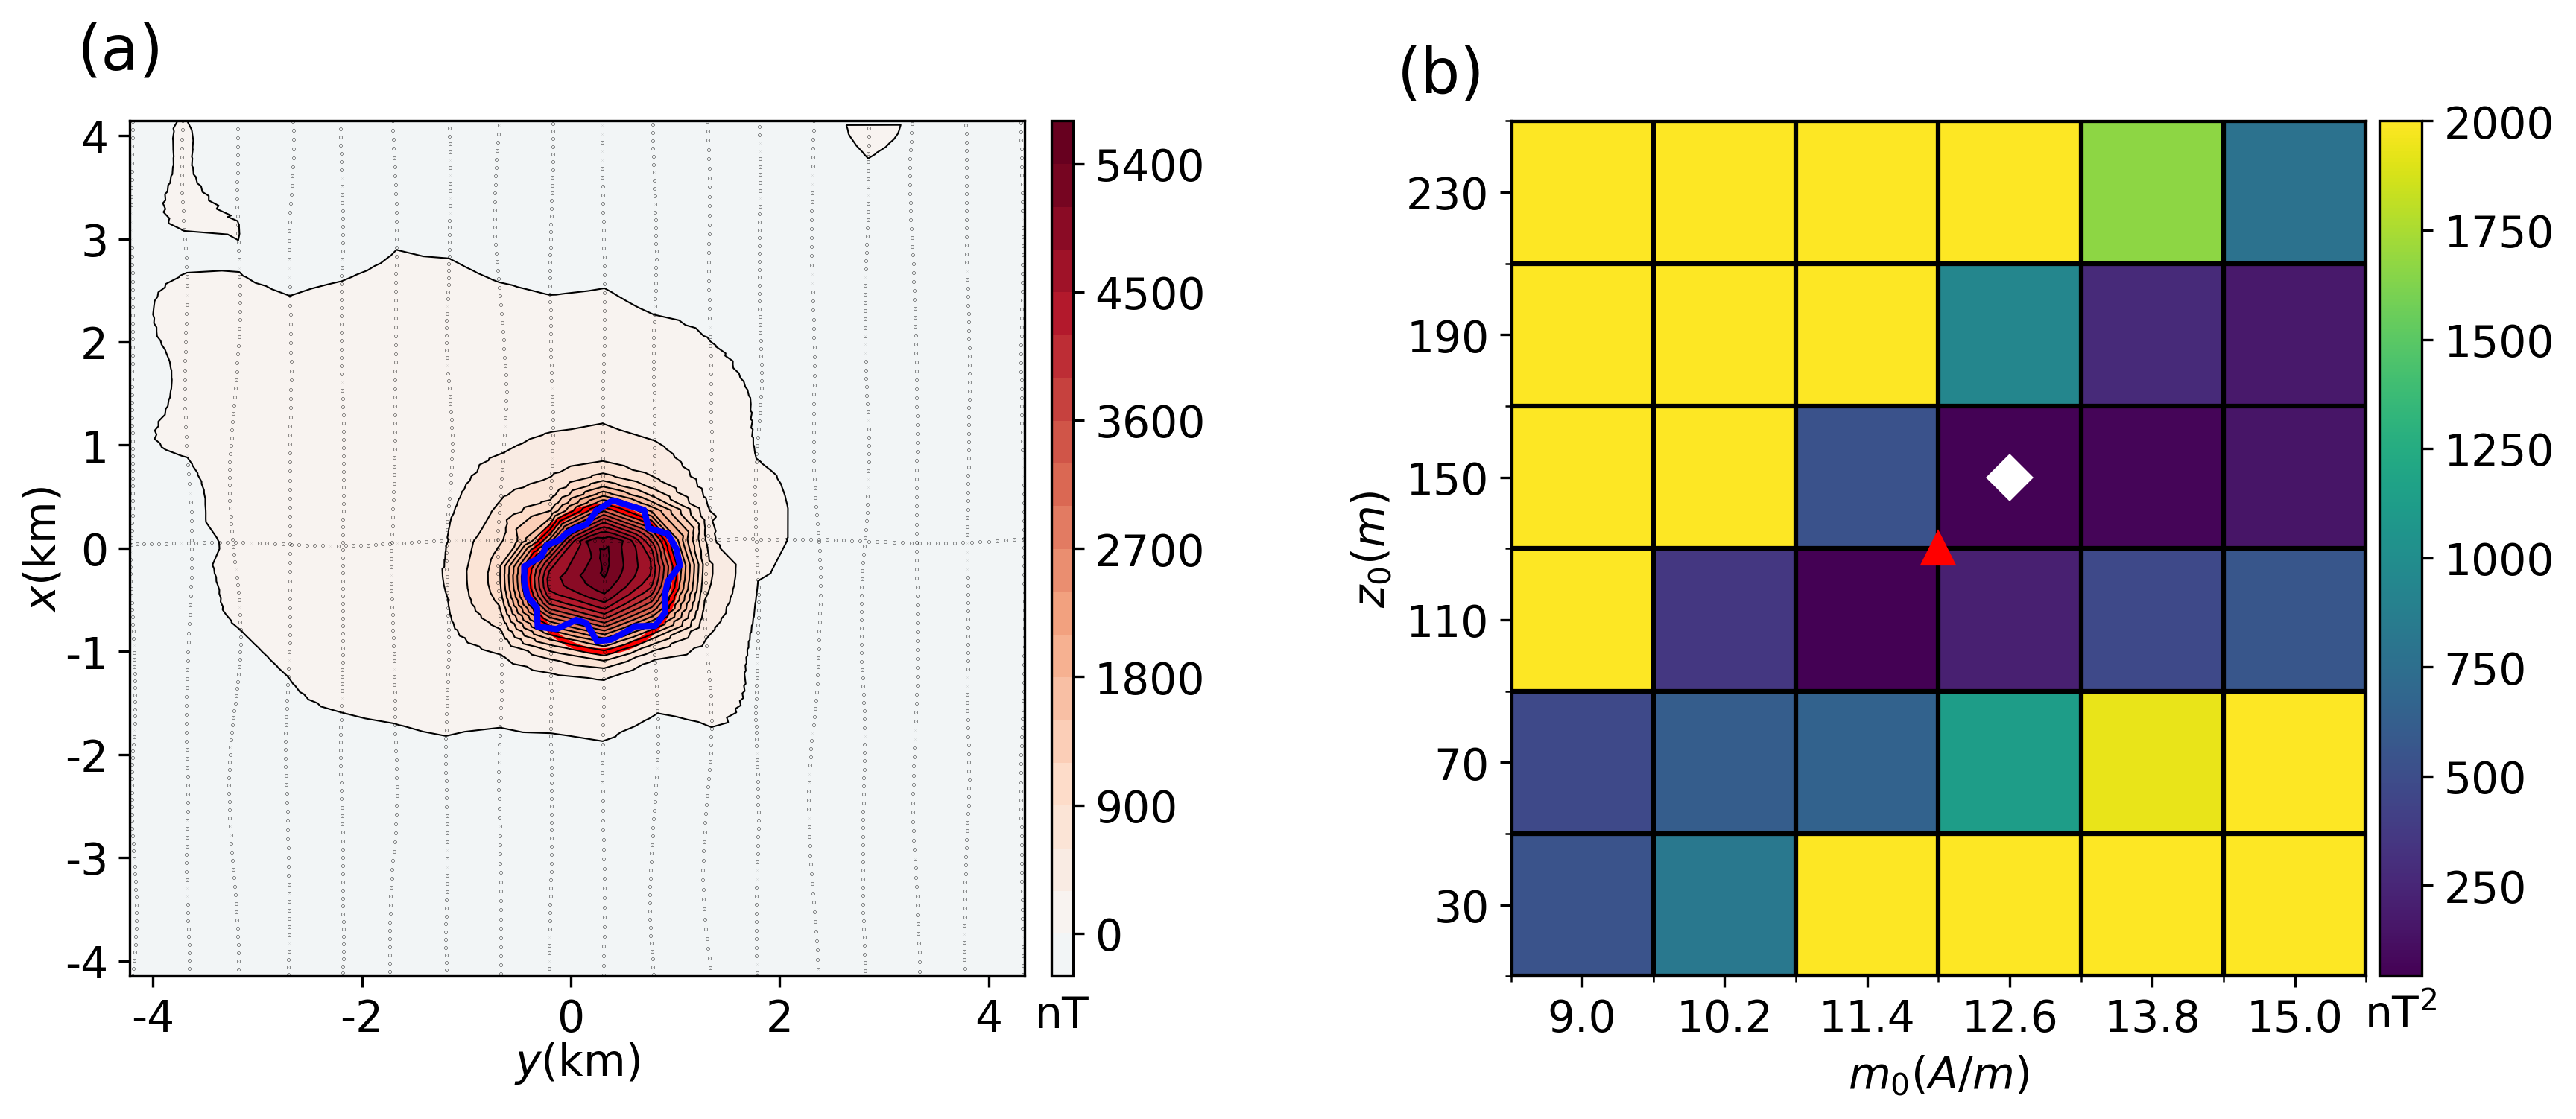
\includegraphics[width=\linewidth]{figures/complex_rtp.png}
    \caption{Complex model simulation. (a) RTP anomaly of the total-field anomaly
    shown in Fig. \ref{fig:complex_model}(a). 
	The red circle and the blue polygon represent the horizontal projections of the
	initial approximation $\hat{\mathbf{p}}_{(0)}$ and  the simulated dipping source,
	respectively.
	(b) Discrete map of the goal function $\Gamma(\mathbf{p}, m_0, z_0)$ (Eq.
	\ref{eq:gamma}) produced by the estimates $\hat{\mathbf{p}}_{(f)}$ obtained with
	a $6 \times 6$ grid of tentative values for depth to the top $z_0$ and
	total-magnetization intensity $m_0$.
	The red triangle and white diamond pinpoint, respectively, the true and
	retrieved values of $m_0$ and $z_0$.     
}
    \label{fig:complex_rtp}
\end{figure}

\begin{figure}
    \centering
    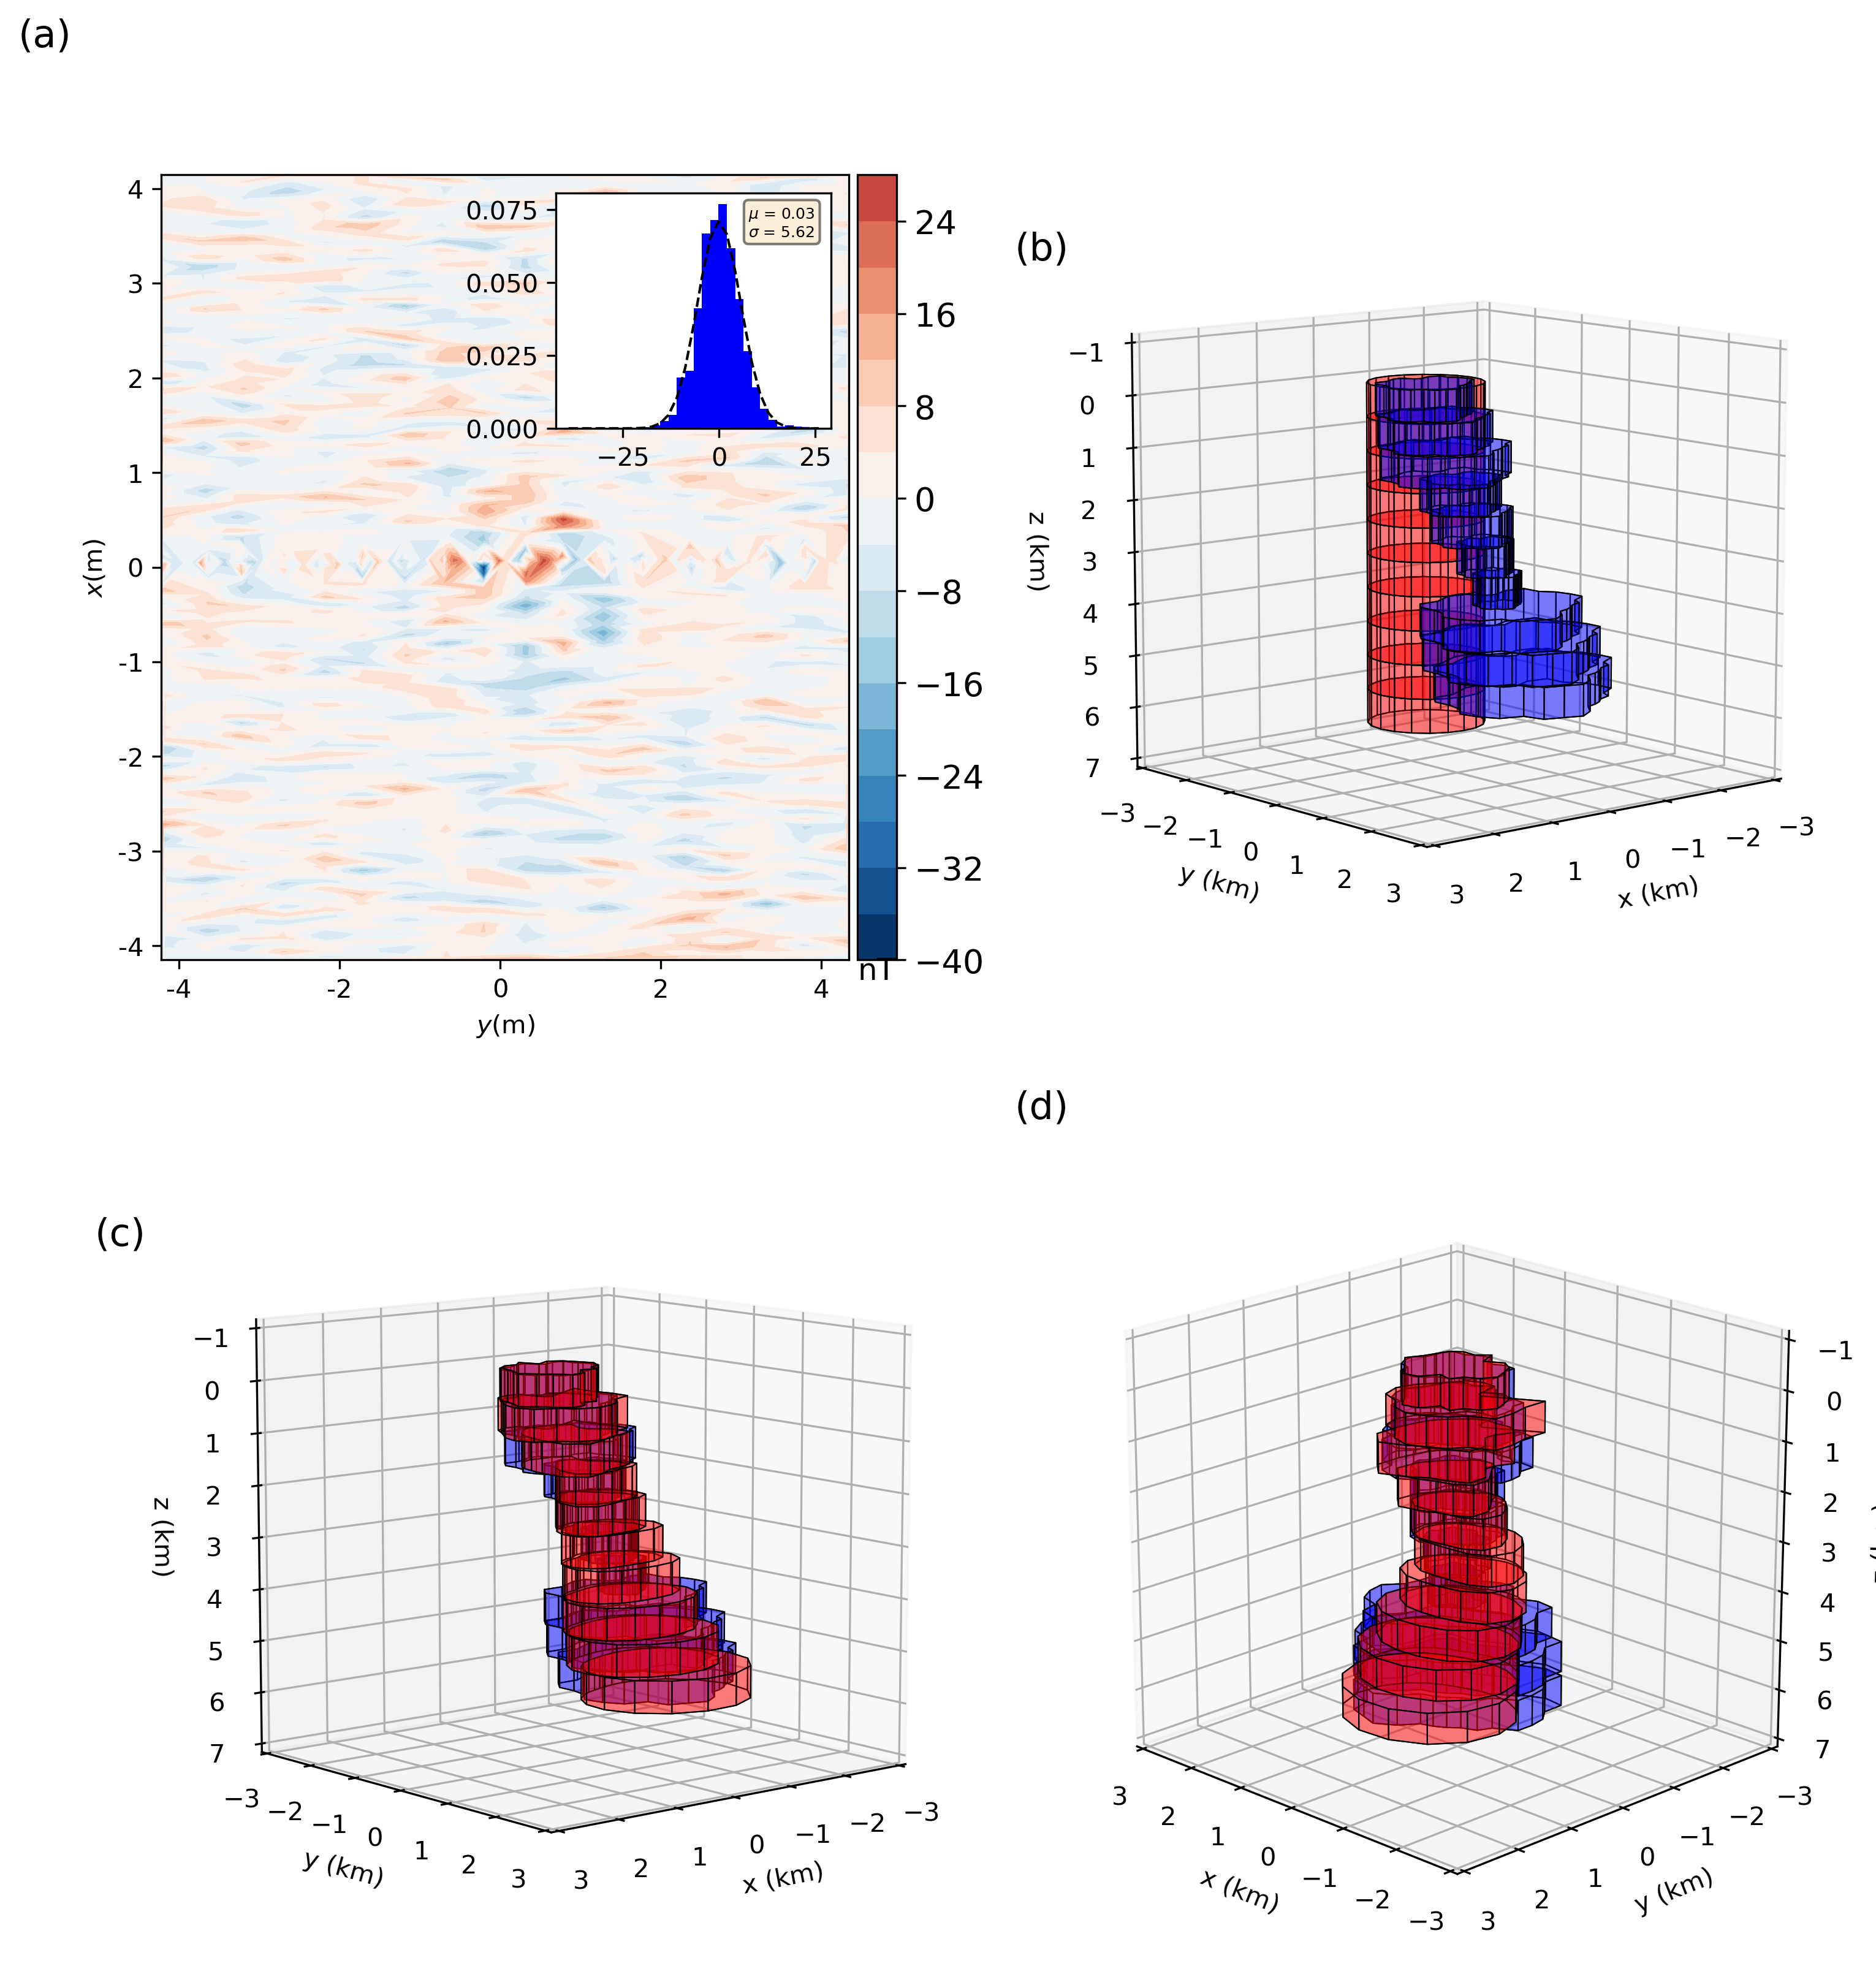
\includegraphics[width=\linewidth]{figures/complex_results.png}
    \caption{Complex model simulation. (a) Residuals between the noise-corrupted data (Fig. \ref{fig:complex_model}a) and the predicted data (not shown) produced by the estimated model (red prisms panels (c) and (d)) using $m_0$  and $z_0$ pinpointed by the white diamond in Fig. \ref{fig:complex_rtp}b.
    The inset shows the histogram of the residuals and the Gaussian curve (dashed line) has mean and standard deviation equal to $\mu = 0.01$ nT and $\sigma=6.6$ nT, respectively.  (b) Perspective view of the initial approximation (red prisms) and the true model (blue prisms). (c) and (d) Comparison between the estimated source (red prisms) and the true model (blue prisms) in perspective views. 
}
    \label{fig:complex_result}
\end{figure}

% Application to field data

\begin{figure}
    \centering
    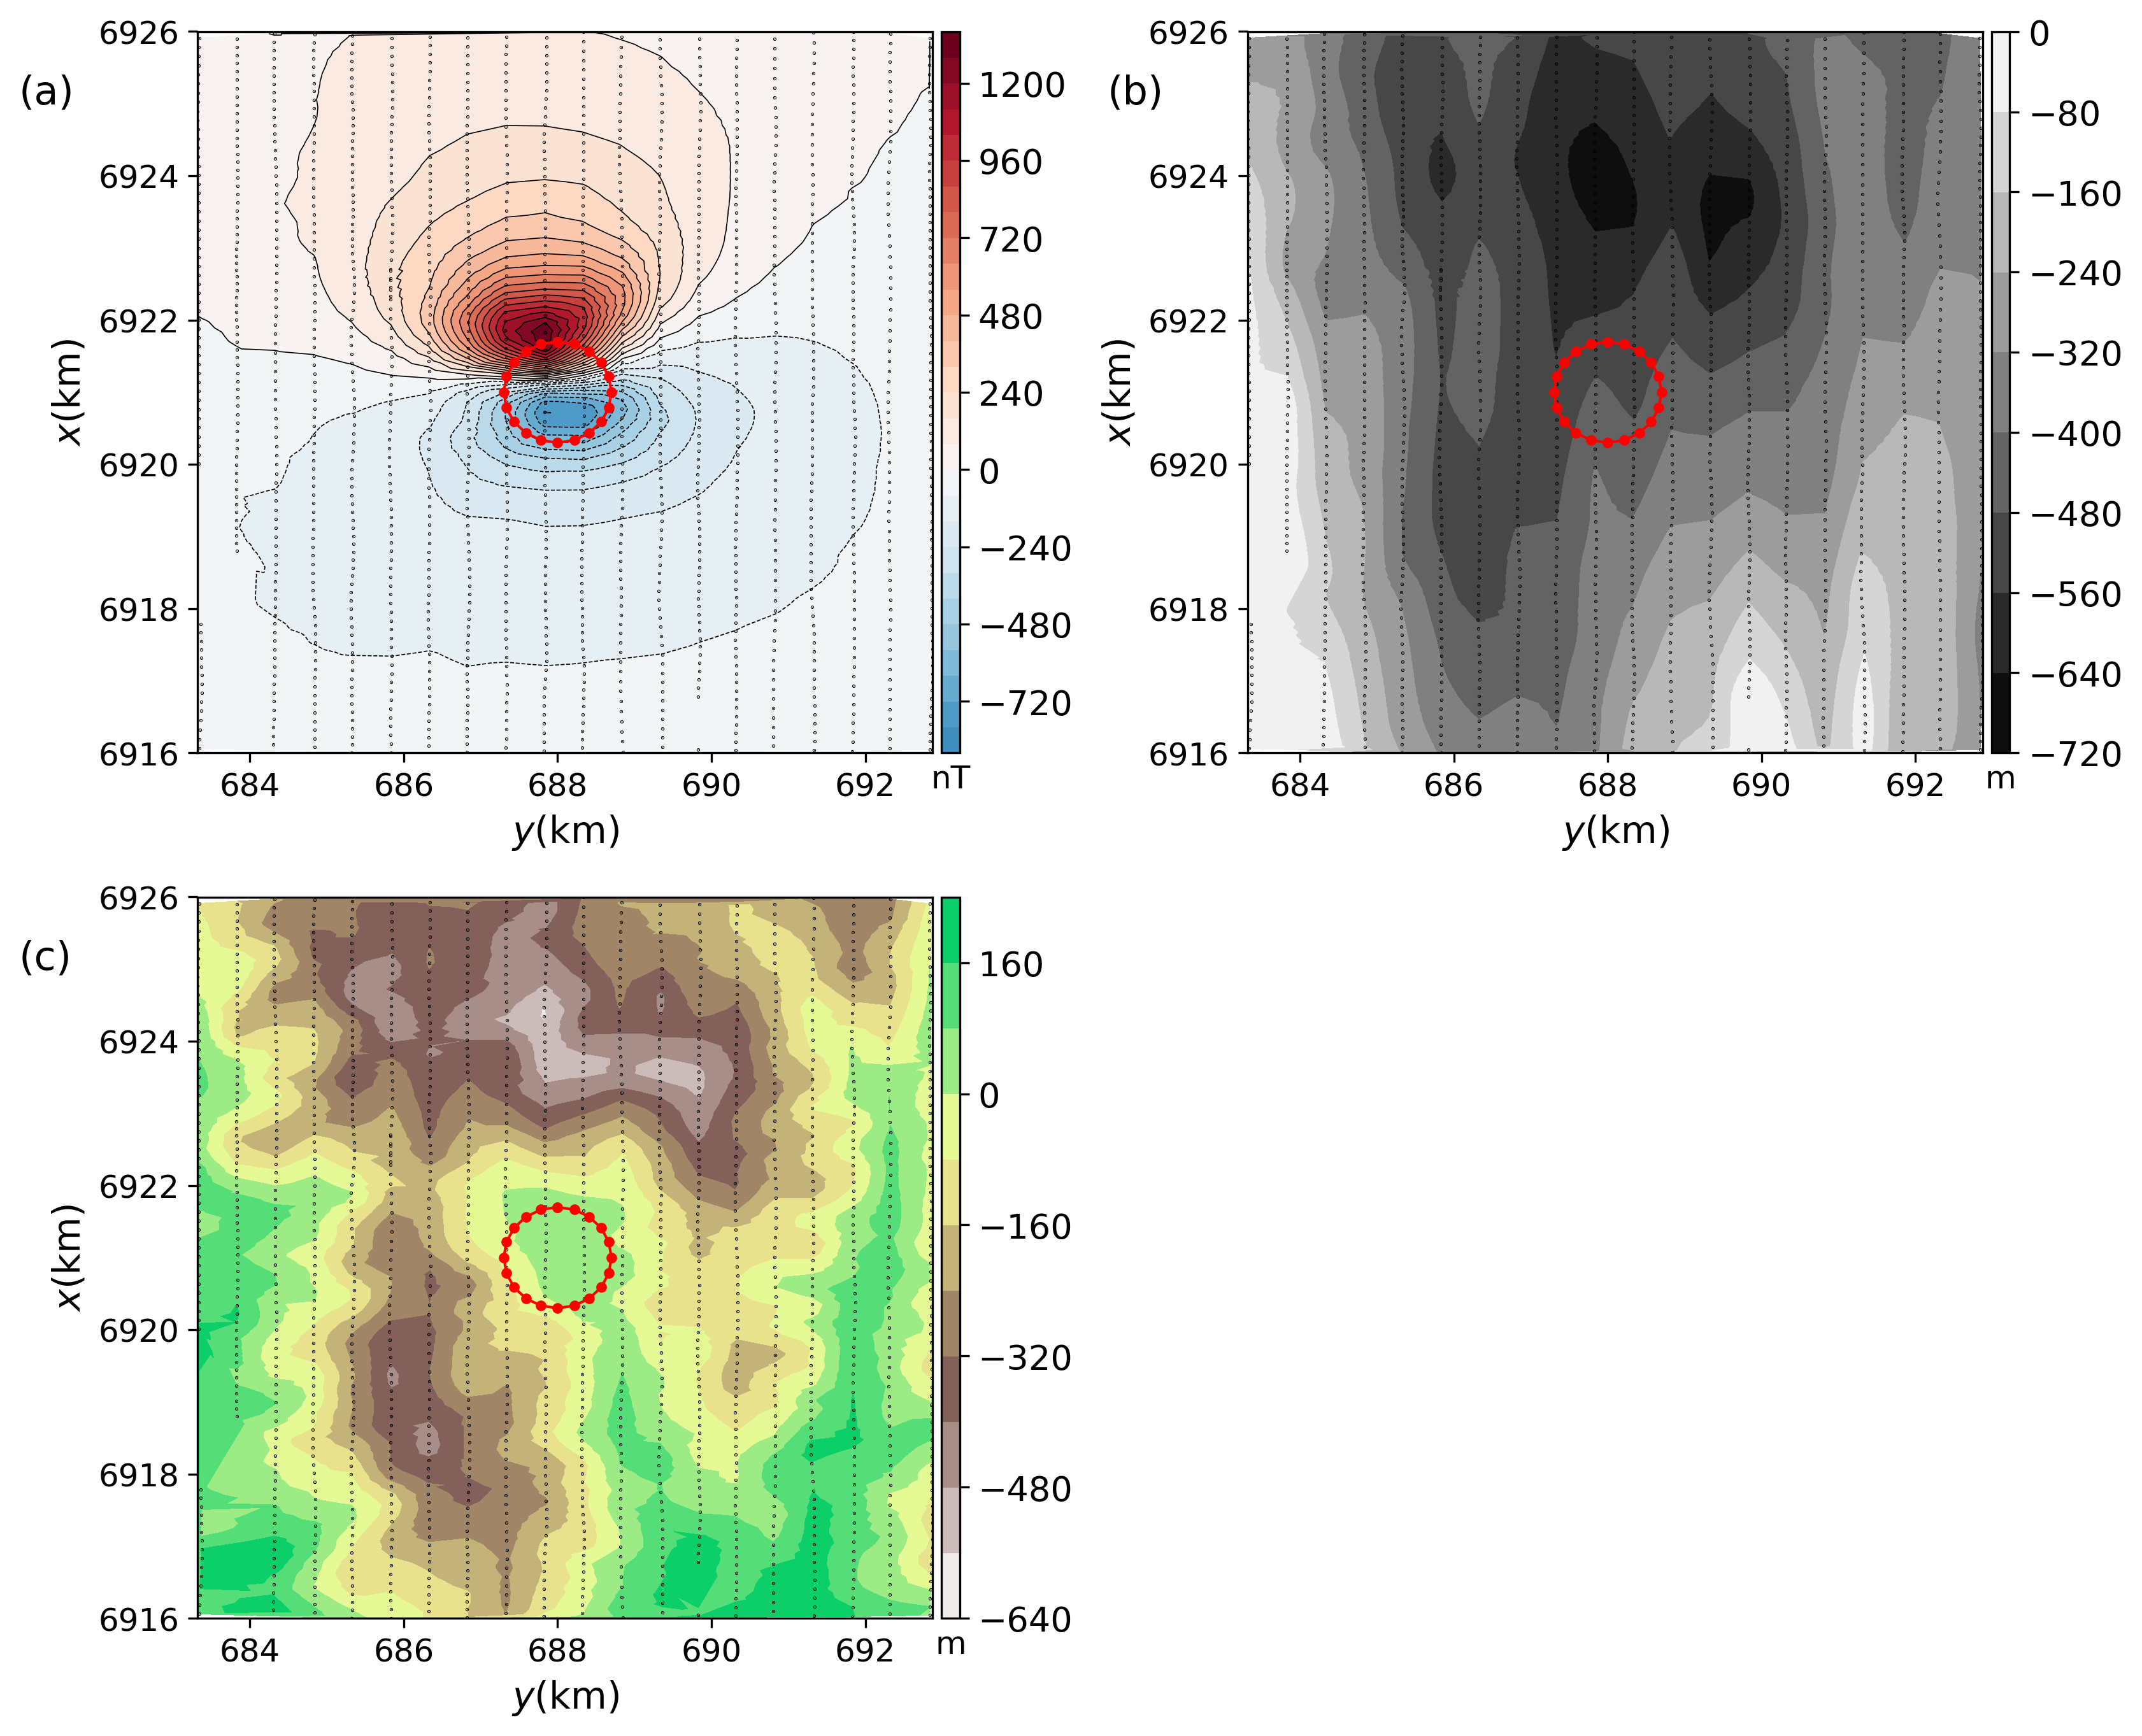
\includegraphics[width=\linewidth]{figures/field_data_alt_topo.png}
    \caption{Application to field data.  (a) Observed total-field anomaly over the  
    Anit{\'a}polis alkaline-carbonatitic complex in southern Brazil. The horizontal UTM 
    coordinates are referred to the central meridian $ 51^\circ $ W. 
    The black dots represent the observation points.
    (b) Regional field using least-squares first-order polynomial fitting. 
    (c) Geometric height of the observation points. (d) Topography of the study area.
    Both of these coordinates are referred to the WGS84 ellipsoid. We have subtracted 
    $ 800 $ m from their values. 
    The magenta rectangle delimits the data to be inverted.
    }
    \label{fig:real_data}
\end{figure}

\begin{figure}
    \centering
    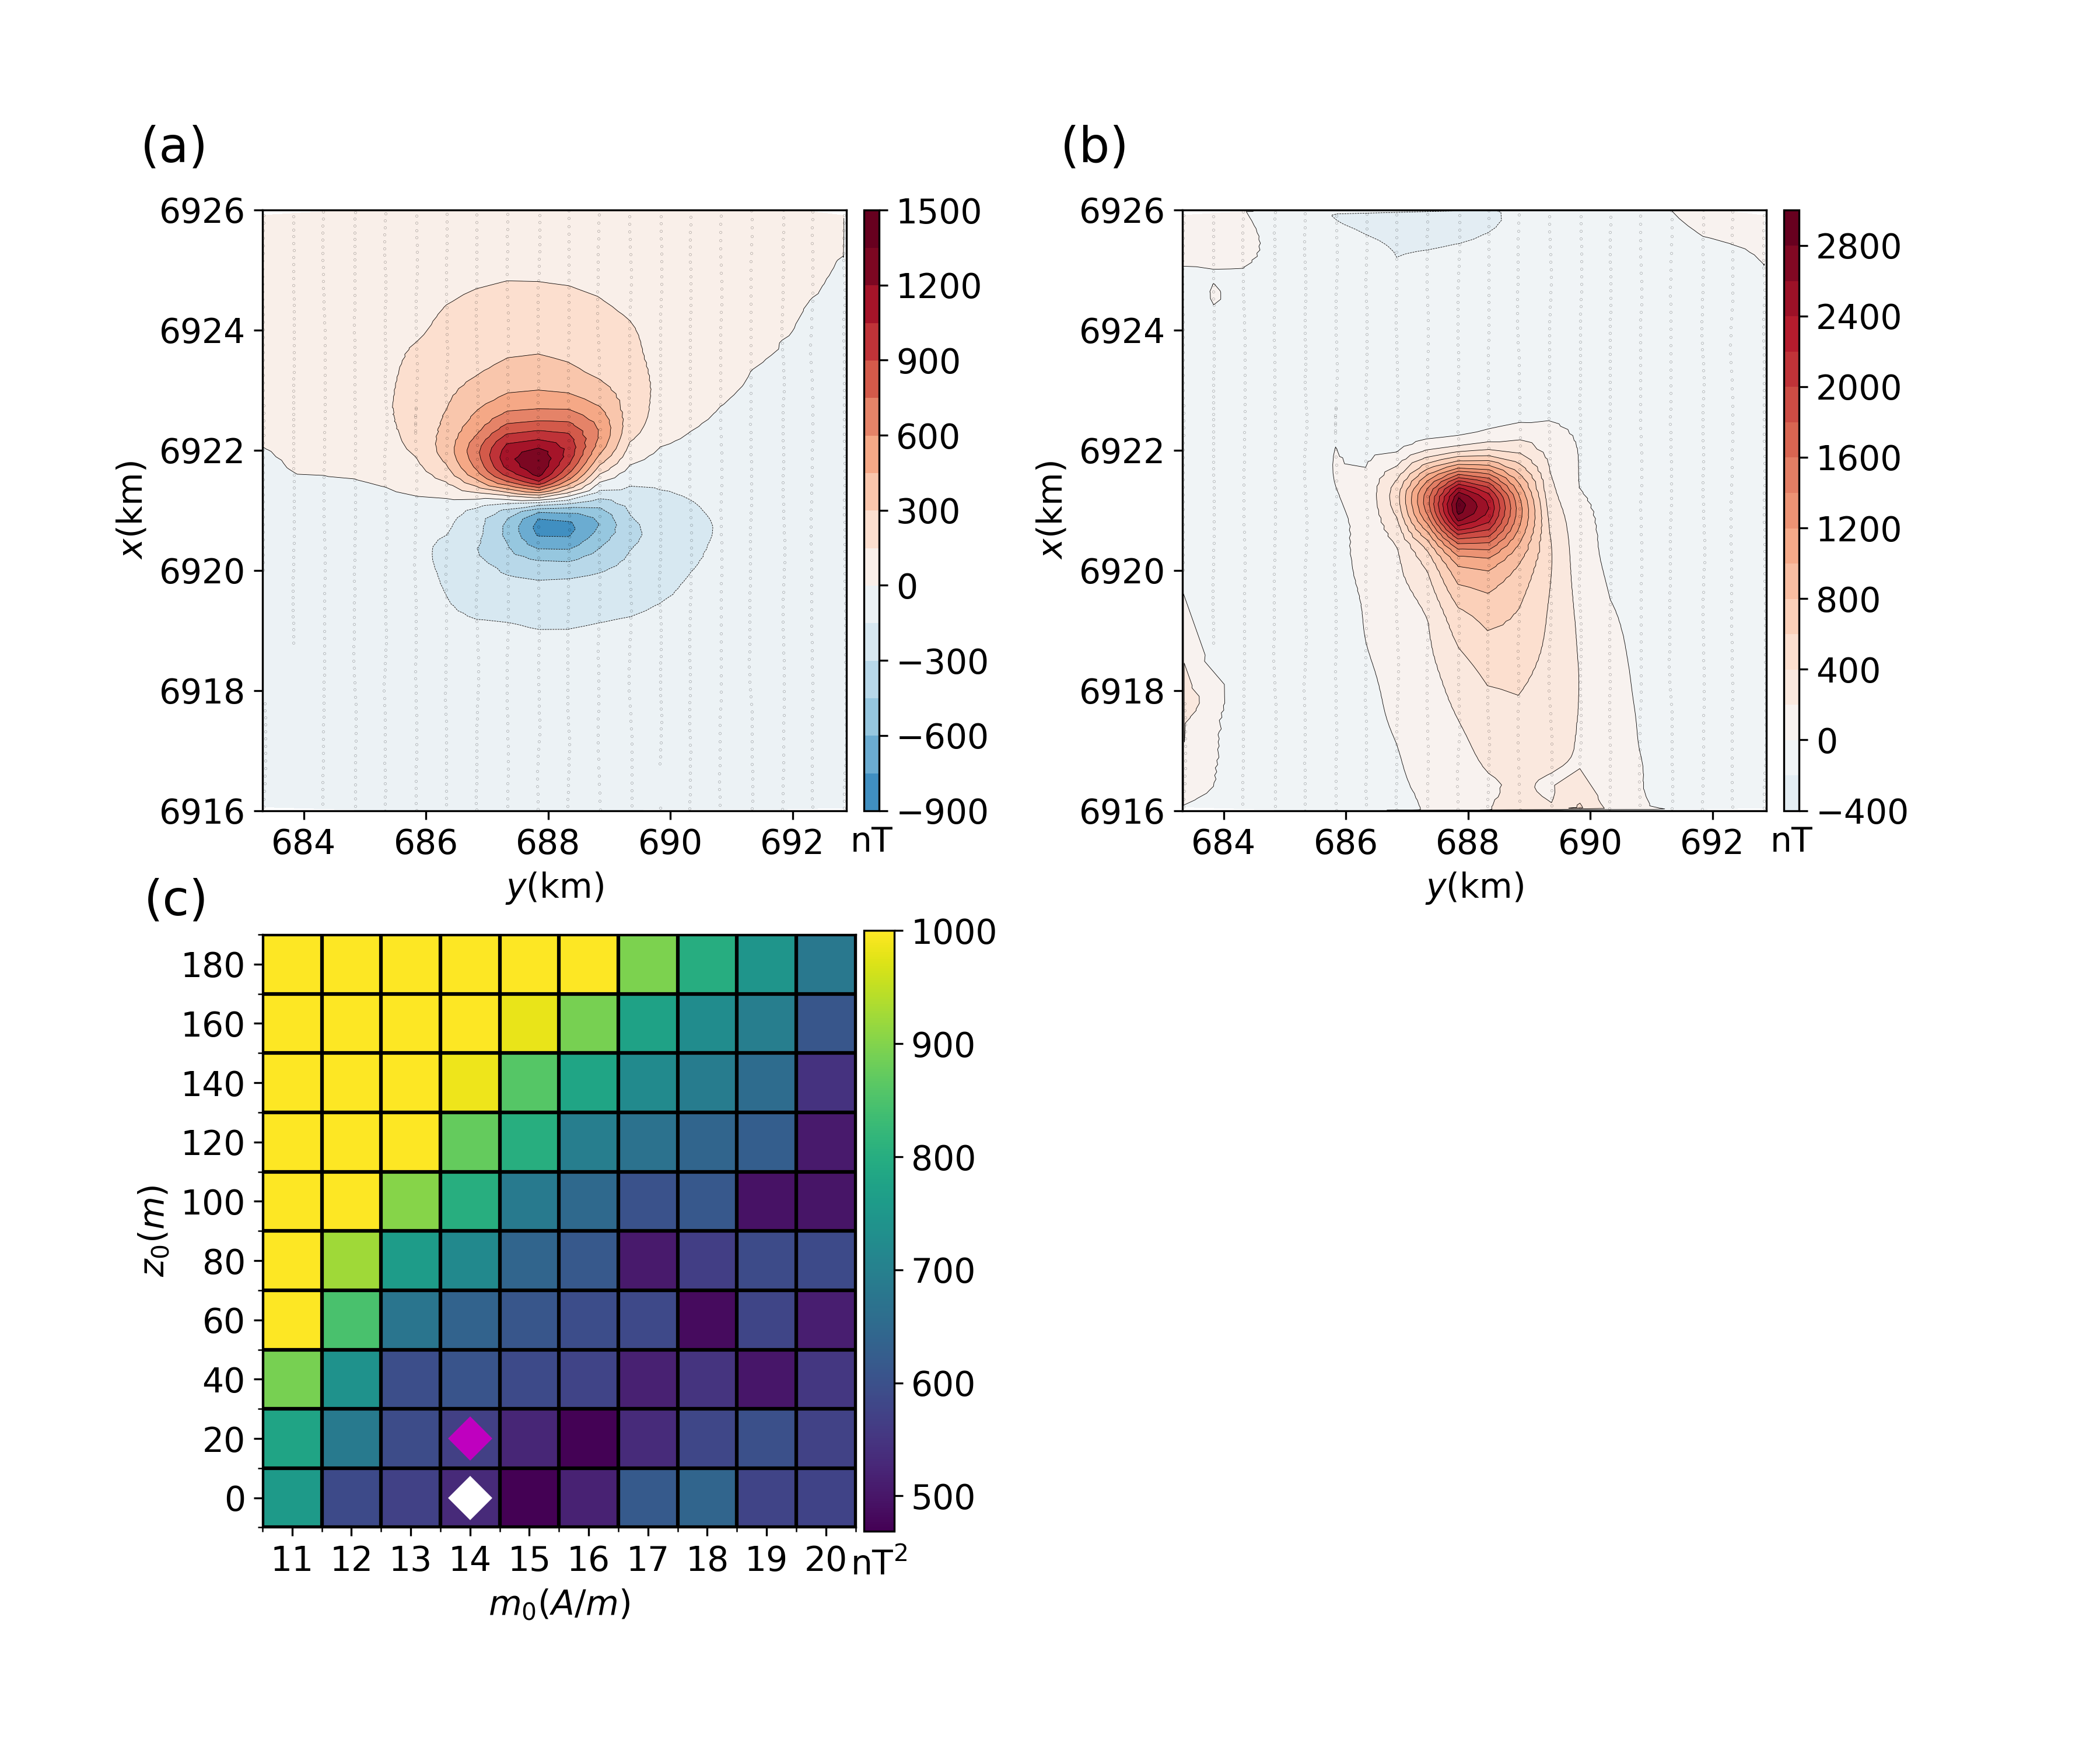
\includegraphics[width=\linewidth]{figures/anitapolis_rtp.png}
    \caption{Application to field data over the Anit{\'a}polis complex, Brazil. 
    (a) Residual total-field anomaly to be inverted over the area delimited by the 
    magenta rectangle in Fig. \ref{fig:real_data}. The red circle represents the
    horizontal projections of the initial approximation $\hat{\mathbf{p}}_{(0)}$.
    (b) RTP anomaly of the  residual total-field anomaly shown in panel (a).
    (c) Discrete map of the goal function $\Gamma(\mathbf{p}, m_0, z_0)$ (Eq.
    \ref{eq:gamma}) produced by the estimates $\hat{\mathbf{p}}_{(f)}$ obtained with
    a $6 \times 6$ grid of tentative values for depth to the top $z_0$ and
    total-magnetization intensity $m_0$.
    The white and magenta diamonds pinpoint, respectively, two pairs of $m_0$ and
    $z_0$ whose goal functions are close to each other. The magenta diamond pinpoints the estimated model that produces the smallest value of 
    $\Gamma(\hat{\mathbf{p}}_{(f)}, m_0, z_0)$.
    The white diamond pinpoints an alternative model whose depth to the top is $z_0=0$ indicating a possible outcropping not corroborated by the literature.	 
}
    \label{fig:anitapolis_rtp}
\end{figure}



\begin{figure}
	\centering
	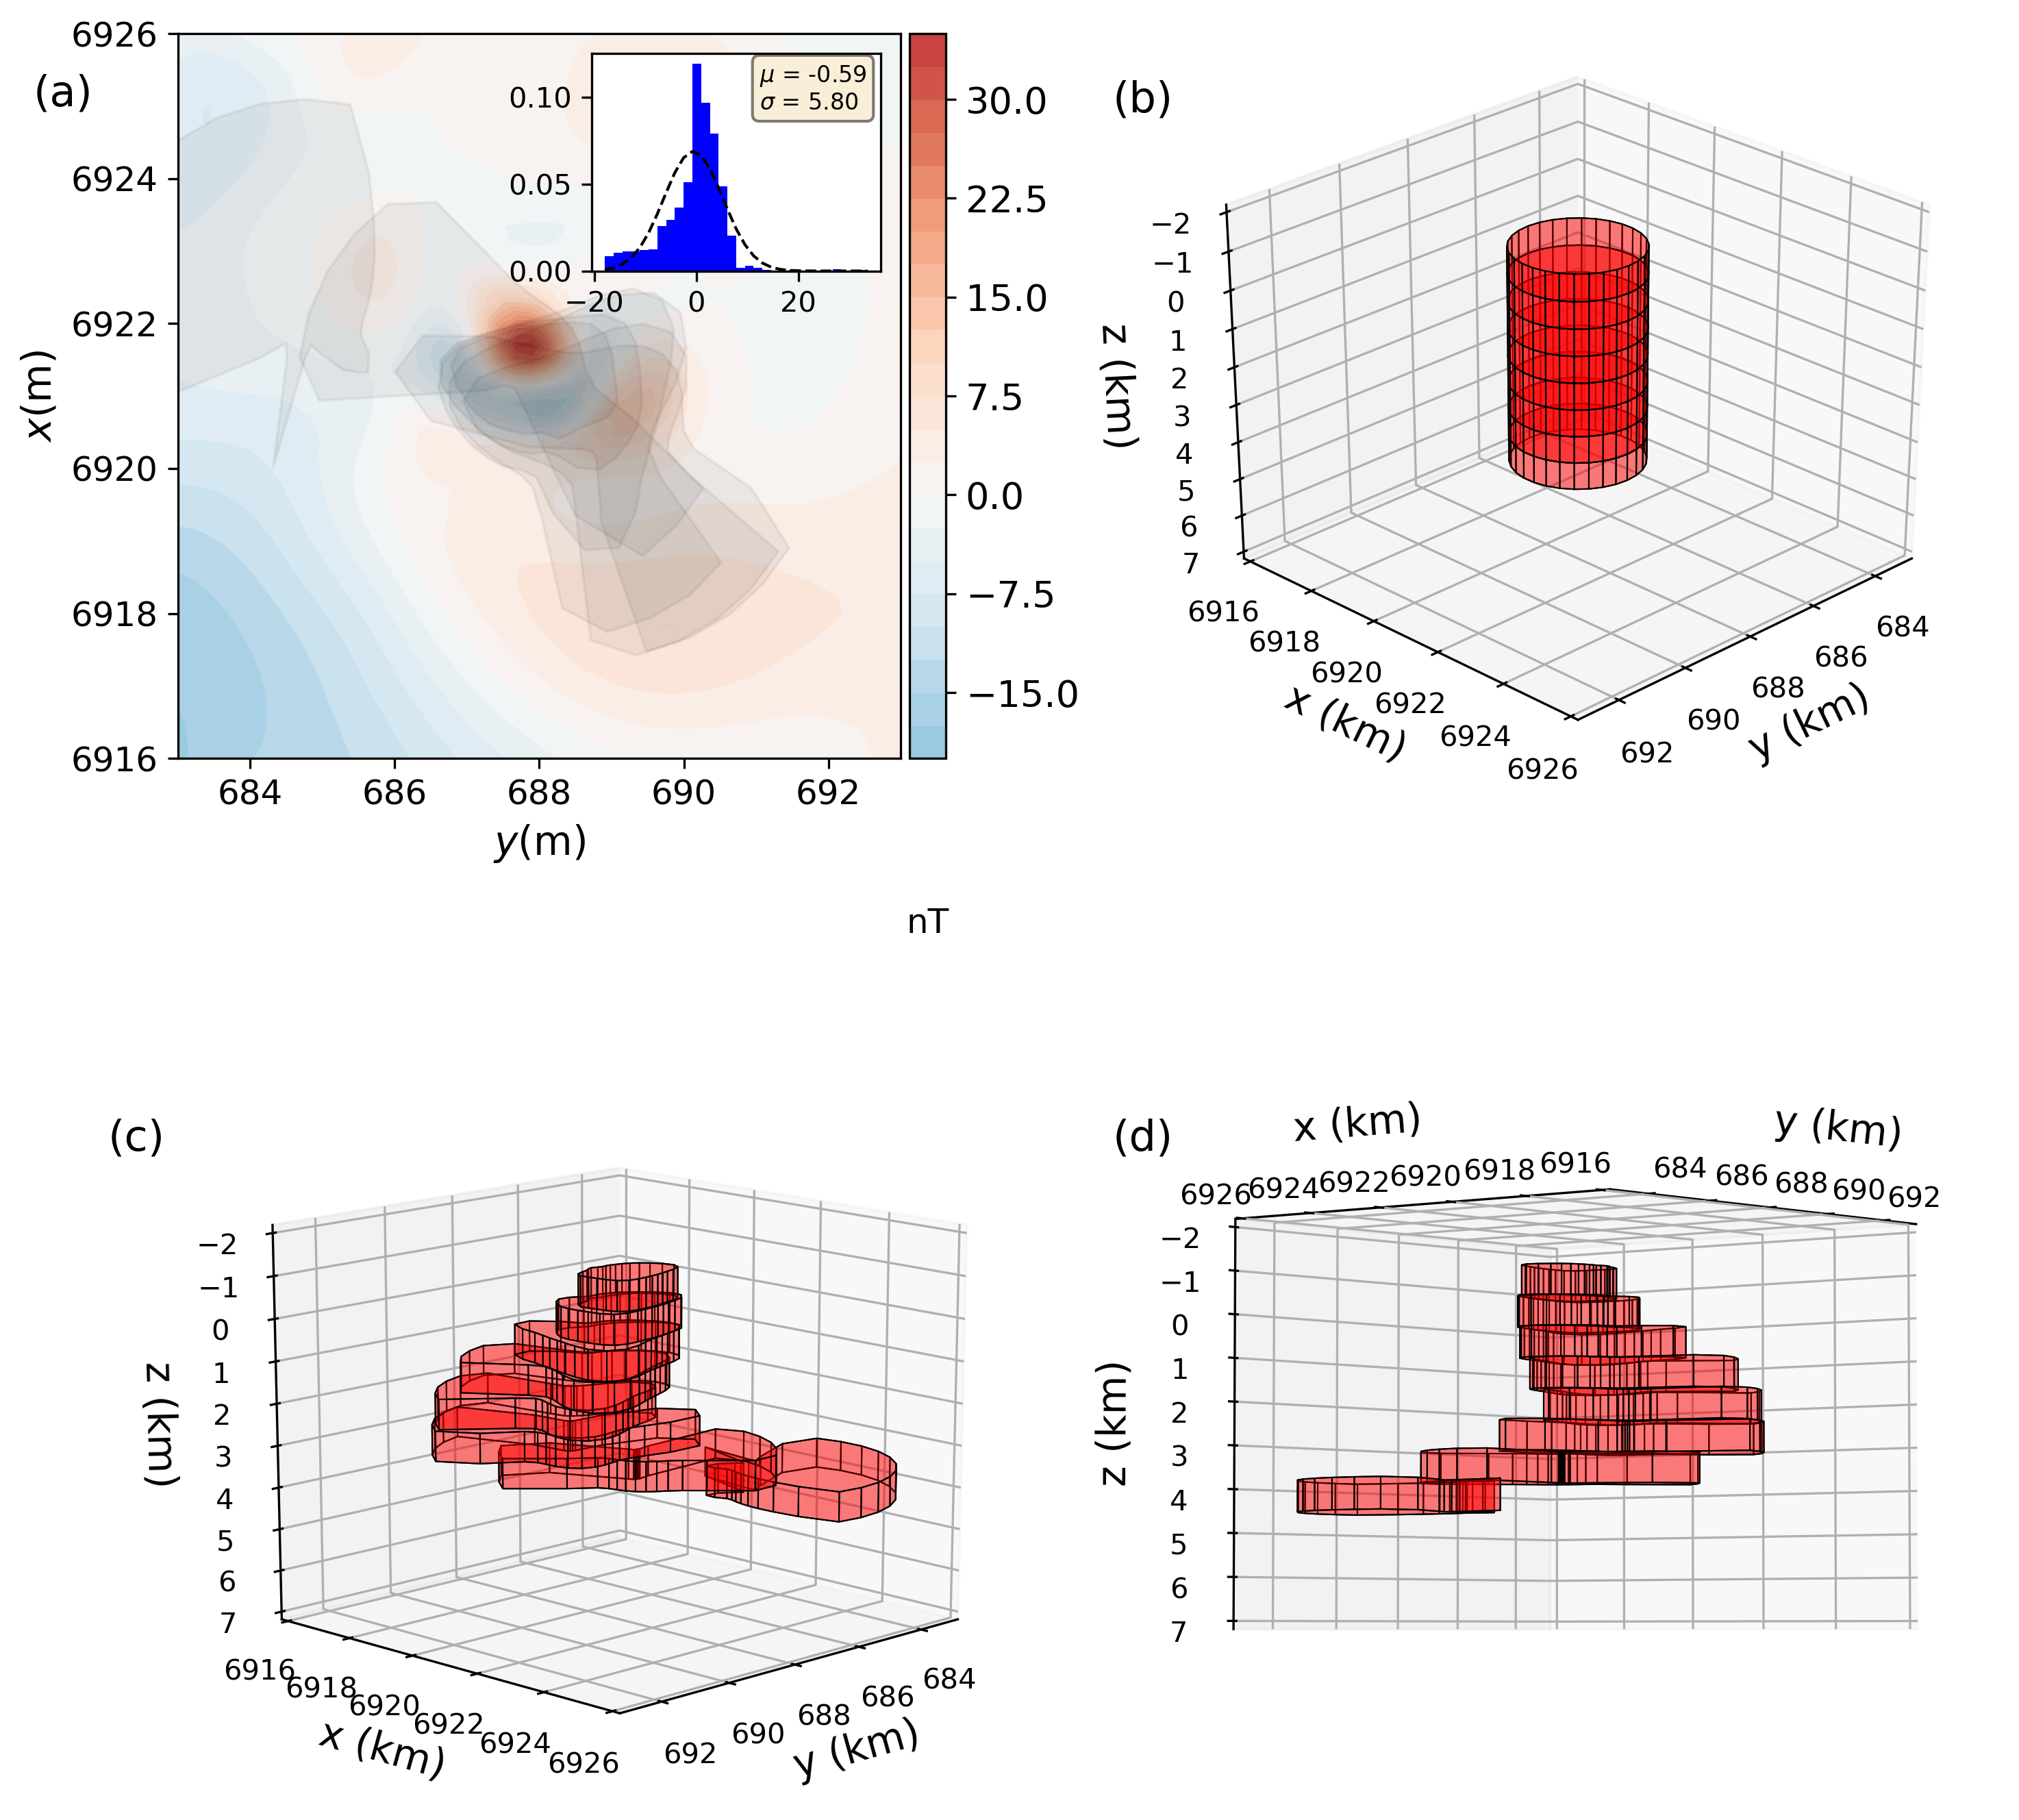
\includegraphics[width=\linewidth]{figures/real_results_magenta_diamond.png}
	\caption{Application to the field data over the Anit{\'a}polis complex, Brazil.
	The non-outcropping estimated model producing the smallest goal function 
	($ \Gamma(\hat{\mathbf{p}}_{(f)}, m_0, z_0)$, Eq. \ref{eq:gamma})	represented by the magenta diamond 
	in Fig. \ref{fig:anitapolis_rtp}c.
	(a) Residuals between the observed data (Fig. \ref{fig:anitapolis_rtp}a) and the 
	predicted data (not shown) produced by the estimated model. 
	The inset shows the histogram of the residuals and the fitted normal 
	Gaussian curve (dashed line) with mean $\mu = -1.2$ nT and 
	standard deviation $\sigma = 20.70$ nT.
	The light-gray polygons represent the horizontal projection of the estimated 
	model onto the residual map. 
	(b) Perspective view of the initial approximation (red prisms). 
	(c) and (d) Perspective views of the estimated model (red prisms).}
	\label{fig:real_result2}
\end{figure}

\begin{figure}
    \centering
    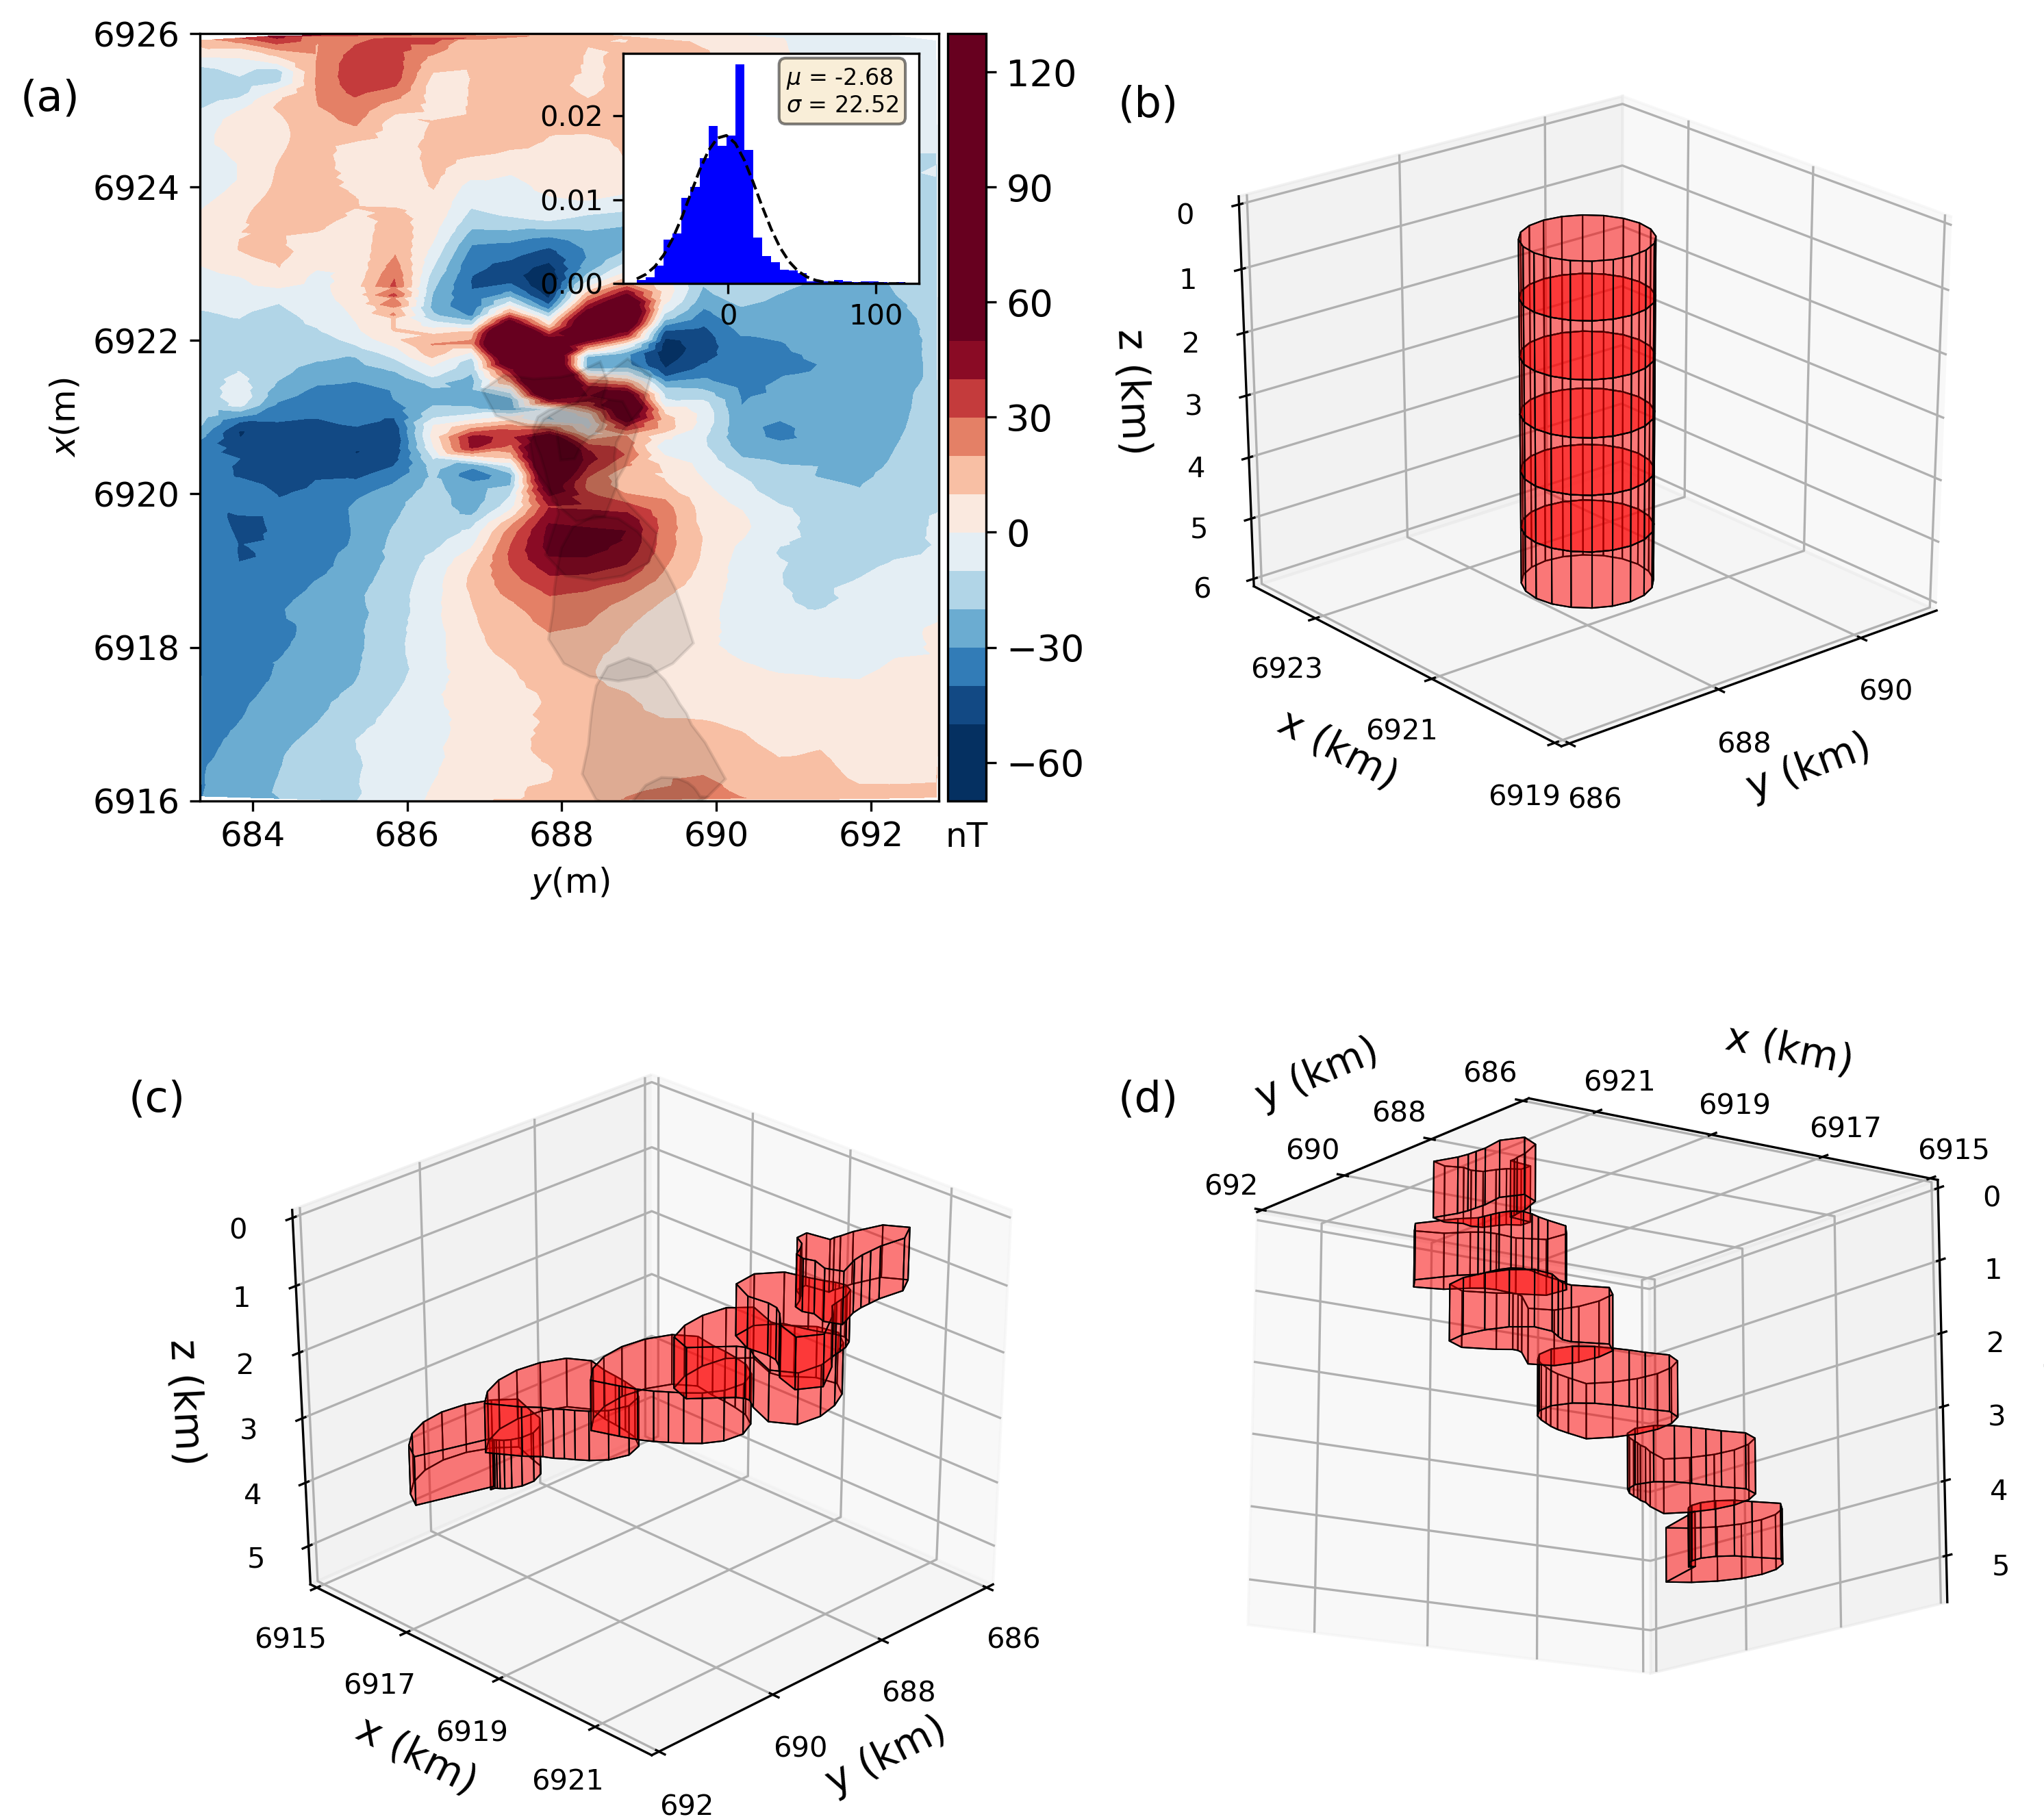
\includegraphics[width=\linewidth]{figures/real_results_white_diamond.png}
    \caption{Application to the field data over the Anit{\'a}polis complex, Brazil.
    Outcropping estimated model  represented by the white diamond in in Fig.    		   \ref{fig:anitapolis_rtp}c. 
    (a) Residuals between the observed data (Fig. \ref{fig:anitapolis_rtp}a and the 
    predicted data (not shown) produced by the estimated model. 
    The inset shows the histogram of the residuals and the fitted normal 
    Gaussian curve (dashed line) with mean $\mu = 1.0$ and standard deviation  
    $\sigma = 20.6$.
    The light-gray polygons represent the horizontal projection of the estimated 
    model onto the residual map. 
    (b) Perspective view of the initial approximation (red prisms). 
    (c) and (d) Perspective views of the estimated model (red prisms).}
    \label{fig:real_result}
\end{figure}

\appendix

\label{lastpage}


\end{document}